% В этом документе преамбула

%%% Работа с русским языком
\usepackage{cmap}					% поиск в PDF
\usepackage{mathtext} 				% русские буквы в формулах
\usepackage[T2A]{fontenc}			% кодировка
\usepackage[utf8]{inputenc}			% кодировка исходного текста
\usepackage[english,russian]{babel}	% локализация и переносы
\usepackage{indentfirst}			% чтобы первый абзац в разделе отбивался красной строкой
\frenchspacing						% тонкая настройка пробелов

%%% Приведение начертания букв и знаков к русской типографской традиции
\renewcommand{\epsilon}{\ensuremath{\varepsilon}}
\renewcommand{\phi}{\ensuremath{\varphi}}			% буквы "эпсилон"
\renewcommand{\kappa}{\ensuremath{\varkappa}}		% буквы "каппа"
\renewcommand{\le}{\ensuremath{\leqslant}}			% знак меньше или равно
\renewcommand{\leq}{\ensuremath{\leqslant}}			% знак меньше или равно
\renewcommand{\ge}{\ensuremath{\geqslant}}			% знак больше или равно
\renewcommand{\geq}{\ensuremath{\geqslant}}			% знак больше или равно
\renewcommand{\emptyset}{\varnothing}				% знак пустого множества

%%% Дополнительная работа с математикой
\usepackage{amsmath,amsfonts,amssymb,amsthm,mathtools} % AMS
\usepackage{icomma} % "Умная" запятая: $0,2$ --- число, $0, 2$ --- перечисление

%% Номера формул
\mathtoolsset{showonlyrefs=true} % Показывать номера только у тех формул, на которые есть \eqref{} в тексте.

%% Свои команды

% операции, не определённые (или имеющие иные обохначения) в мат. пакетах
\DeclareMathOperator{\sgn}{\mathop{sgn}}				% ф-ия sgn
\renewcommand{\tg}{\mathop{\mathrm{tg}}\nolimits}		% обозначение тангенса

%% Перенос знаков в формулах (по Львовскому)
\newcommand*{\hm}[1]{#1\nobreak\discretionary{}
{\hbox{$\mathsurround=0pt #1$}}{}}

%%% Работа с картинками
\usepackage{graphicx}  % Для вставки рисунков
\graphicspath{{images/}{images2/}}  % папки с картинками
\setlength\fboxsep{3pt} % Отступ рамки \fbox{} от рисунка
\setlength\fboxrule{1pt} % Толщина линий рамки \fbox{}
\usepackage{wrapfig} % Обтекание рисунков текстом

%%% Работа с таблицами
\usepackage{array,tabularx,tabulary,booktabs} % Дополнительная работа с таблицами
\usepackage{longtable}  % Длинные таблицы
\usepackage{multirow} % Слияние строк в таблице

%%% Теоремы
\theoremstyle{plain} % Это стиль по умолчанию, его можно не переопределять.
\newtheorem{theorem}{Теорема}[section]
\newtheorem{lemma}{Лемма}[section]
\newtheorem{definition}[theorem]{Определение}
\newtheorem{property}{Свойство}
 
\theoremstyle{definition} % "Определение"
\newtheorem{corollary}{Следствие}[theorem]
\newtheorem{exmp}{Пример}[section]
 
\theoremstyle{remark} % "Примечание"
\newtheorem*{nonum}{Решение}
\newtheorem*{evidence}{Доказательство}
\newtheorem*{remark}{Примечание}

%%% Программирование
\usepackage{etoolbox} % логические операторы

%%% Страница
\usepackage{extsizes} % Возможность сделать 14-й шрифт
\usepackage{geometry} % Простой способ задавать поля
	\geometry{top=25mm}
	\geometry{bottom=35mm}
	\geometry{left=35mm}
	\geometry{right=20mm}

%\usepackage{fancyhdr} % Колонтитулы
% 	\pagestyle{fancy}
 	%\renewcommand{\headrulewidth}{0pt}  % Толщина линейки, отчеркивающей верхний колонтитул
% 	\lfoot{Нижний левый}
% 	\rfoot{Нижний правый}
% 	\rhead{Верхний правый}
% 	\chead{Верхний в центре}
% 	\lhead{Верхний левый}
%	\cfoot{Нижний в центре} % По умолчанию здесь номер страницы

\usepackage{setspace} % Интерлиньяж (межстрочные интервалы)
%\onehalfspacing % Интерлиньяж 1.5
%\doublespacing % Интерлиньяж 2
%\singlespacing % Интерлиньяж 1

\usepackage{lastpage} % Узнать, сколько всего страниц в документе.

\usepackage{soulutf8} % Модификаторы начертания

\usepackage{hyperref}
\usepackage[usenames,dvipsnames,svgnames,table,rgb]{xcolor}
\hypersetup{				% Гиперссылки
    unicode=true,           % русские буквы в раздела PDF
    pdftitle={Заголовок},   % Заголовок
    pdfauthor={Автор},      % Автор
    pdfsubject={Тема},      % Тема
    pdfcreator={Создатель}, % Создатель
    pdfproducer={Производитель}, % Производитель
    pdfkeywords={keyword1} {key2} {key3}, % Ключевые слова
    colorlinks=true,       	% false: ссылки в рамках; true: цветные ссылки
    linkcolor=MidnightBlue,          % внутренние ссылки
    citecolor=black,        % на библиографию
    filecolor=magenta,      % на файлы
    urlcolor=blue           % на URL
}

\usepackage{csquotes} % Еще инструменты для ссылок

%\usepackage[style=authoryear,maxcitenames=2,backend=biber,sorting=nty]{biblatex}

\usepackage{multicol} % Несколько колонок

%%% Работа с графикой
\usepackage{tikz}
\usetikzlibrary{calc}
\usepackage{tkz-euclide}
\usetikzlibrary{arrows}
\usepackage{pgfplots}
\usepackage{pgfplotstable}

%%% Настройка подписей к плавающим объектам
\usepackage{floatrow}	% размещение
\usepackage{caption}	% начертание
\captionsetup[figure]{labelfont=bf,textfont=it,font=footnotesize}	% нумерация и надпись курсивом
% для подфигур: заголовок подписи полужирный, текст заголовка обычный
% выравнивание является неровным (т.е. выровненным по левому краю)
% singlelinecheck = off означает, что настройка выравнивания используется, даже если заголовок имеет длину только одну строку.
% если singlelinecheck = on, то заголовок всегда центрируется, когда заголовок состоит только из одной строки.
\captionsetup[subfigure]{labelfont=bf,textfont=normalfont,singlelinecheck=off,justification=raggedright}

%%% Stuff для графиков и рисунков



\begin{document} % начало документа

\thispagestyle{empty}
\begin{center}
	\textbf{Санкт-Петербургский государственный электротехнический университет \\ <<,,\hspace{0.5pt}ЛЭТИ\hspace{0.5pt}`` имени В. И. Ульянова (Ленина)>>}
\end{center}
% выделение имени, тут отступ
\vspace{13ex}
\begin{flushright} % окружение выравнивания по правому краю
	\noindent % убираем отступ для красной строки
	\textit{Почаев Никита Алексеевич}
	\\
	\textit{студент ФКТИ \\(группа 8381)}
	\\
	\textit{Лектор: Малов Сергей Васильевич}
\end{flushright}
\begin{center}
	\vspace{13ex}
	\so{\textbf{КОНСПЕКТ}}
	\vspace{1ex}
	
	по теории вероятностей и математической статистике
	
	
	за 4-ый семестр
	
	
	\vfill % вертикальный пробел, чтобы всё, что до него и до перехода на новую страницу оказалось внизу страницы
	{\small Санкт-Петербург, 2020}
\end{center}
\newpage

\tableofcontents

\newpage

\section{Комбинаторика}

\textbf{Комбинаторные объекты} - конечные множества, на элементы которых могут накладываться определённые ограничения, такие как: различимость или неразличимость элементов, возможность повторения одинаковых элементов и т. п.

Если два комбинаторных объекта, различающихся только порядком элементов, считаются различными, то они называются \textbf{упорядоченными}, т.е. каждому элементу набора сопоставлен номер $\overline{1,n}$ (указано, какие элементы следуют за какими (какие элементы больше каких) - задано отношение порядка).
Обозначение: $(a_1, a_2, ..., a_n) \eq $
\begin{table}[h]
	\begin{tabular}{|l|l|l|l|}
		$a_1$ & $a_2$ & $\dots$ & $a_n$ \\ \hline
	\end{tabular}
\end{table}

\textbf{Неупорядоченный набор}: $\{ a_1, a_2, \dots, a_n \} \eq $
\begin{table}[h]
	\begin{tabular}{|llll|}
		$a_1$ & $a_2$ & $\dots$ & $a_n$ \\ \hline
	\end{tabular}
\end{table}

\begin{remark}
	Оба типа наборов могут содержать повторения.
\end{remark}

\subsection{Принципы комбинаторики}

\textbf{Принцип суммы.}

Если некоторый объект $A$ можно выбрать $n$ способами, а другой объект $B$ можно выбрать $m$ способами, то выбор <<либо $A$, либо $B$>> можно осуществить $n+m$ способами.

$C_1, C_2$ - типы комбинаций. $C = C_1 \cup C_2$ при этом $C_1 \cap C_2 = \emptyset \Rightarrow \# C = \# C_1 + \# C_2$ (где $\#$ - число возможных комбинаций).

\textbf{Принцип произведения.}

Если объект $A$ можно выбрать $n$ способами, а после каждого такого выбора второй объект $B$ можно выбрать (независимо от выбора объекта $A$) $m$ способами, то пары объектов $A$ и $B$  можно выбрать $n \cdot m$ способами.

\begin{definition}[Упорядоченная пара]
	Если задана пара $\{a,b\}$, то множество $\{ \{a\}, \{a,b\} \}$ называется упорядоченной парой и обозначается $(a, b)$. При этом элемент $a$ - называется первым элементом, а элемент $b$ - вторым элементом пары.
\end{definition}

Если $C$ - упорядоченный набор 2-х элементов $(a_1, b_2)$ то
\begin{enumerate}
	\item Число различных вариантов выбора $a_1 = m$
	\item При каждом фиксированном $a_1$, число элементов $C = (a_1, \cdot)$ равно $k$.
\end{enumerate}
Тогда упорядоченную пару элементов можно составить $\# C = m \cdot k$.

Данный факт можно распространить на $n$ элементов:
\begin{table}[h]
	\begin{tabular}{lllll}
		\cline{1-4}
		\multicolumn{1}{|l|}{$(a_1,b_1)$}  & \multicolumn{1}{l|}{$(a_1,b_2)$} & \multicolumn{1}{l|}{$\dots$} & \multicolumn{1}{l|}{$(a_1,b_n)$} & $a_1$   \\ \cline{1-4}
		\multicolumn{1}{|l|}{$(a_2, b_1)$} & \multicolumn{1}{l|}{}            & \multicolumn{1}{l|}{}        & \multicolumn{1}{l|}{}            & $a_2$   \\ \cline{1-4}
		\multicolumn{1}{|l|}{$\dots$}      & \multicolumn{1}{l|}{}            & \multicolumn{1}{l|}{}        & \multicolumn{1}{l|}{}            & $\dots$ \\ \cline{1-4}
		\multicolumn{1}{|l|}{$(a_n,b_1)$}  & \multicolumn{1}{l|}{}            & \multicolumn{1}{l|}{}        & \multicolumn{1}{l|}{}            & $a_n$   \\ \cline{1-4}
		$b_1$                              & $b_2$                            & $\dots$                      & $b_n$                            &        
	\end{tabular}
\end{table}

\begin{remark}
	Все элементы входят в таблицу, пустых ячеек нет.
\end{remark}

~

\textbf{Перестановки} (\textit{англ}. permutations) - упорядоченный набор чисел (элементов) $1,2,\dots,n$, обычно трактуемый как биекция\footnote{Биекция - взаимно-однозначное отображение (соответствие). При биективном отображении каждому элементу одного множества соответствует ровно один элемент другого множества, при этом определено обратное отображение, которое обладает тем же свойством.} на множестве $\{ 1,2,\dots,n \}$, которая числу $i$ ставит соответствие $i$-й элемент из набора.
Примером перестановки может служить задача о рассадке $n$ человек за стол по $n$ местам.

Число перестановок $n(n-1)(n-2) \cdot \dots \cdot 2 \cdot 1 = n!$, действительно:
\begin{itemize}
	\item на первое место может быть любой из $n$ элементов;
	\item на вторую позицию может быть помещен любой из оставшихся $(n-1)$ элементов (итого вариантов $n \cdot (n-1)$);
	\item если продолжить данную последовательность для всех $n$ мест, то получим: $n \cdot (n-1) \cdot (n-2) \cdot ... \cdot 1$, то есть действительно $n!$ (согласно принципу умножения).
\end{itemize}

\textbf{Перестановки с повторениями} (\textit{англ.} permutations with repetitions) — те же перестановки, однако некоторые элементы могут встречаться несколько раз. Рассмотрим следующие задачи, иллюстрирующие данной понятие:
\begin{enumerate}
	\item Пусть имеется $n$ различных шаров и $k$ ящиков. Сколькими способами можно разложить шары по ящикам так, чтобы $n_1$ шаров оказались в первом ящике, $n_2$ шаров - во втором,..., $n_k$ шаров - в $k$-ом ящике: $n = n_1 + n_2 + \dots + n_k$.
	\item Пусть имеется n объектов различных типов: $n_1$ объектов первого типа, $n_2$ объектов второго типа,... $n_k$ объектов $k$-го типа. Сколькими способами можно выбрать позиции под объекты определенной группы?
\end{enumerate}
Будем переставлять $n$ объектов всеми возможными способами (их будет $n!$). Но так как некоторые объекты совпадают, итоговое число будет меньше. В частности, $n_1$ объектов первого типа можно переставлять между собой $n_1!$ способами, но они не меняют итоговую перестановку. Аналогично для всех остальных объектов, поэтому число перестановок с повторениями есть
\[ P_n (n_1,n_2,...,n_k)=\frac{n!}{n_1! \cdot n_2!\cdot ... \cdot n_k!} = \frac{(n_1 + n_2 + \dots + n_k)!}{n_1! \cdot n_2!\cdot ... \cdot n_k!} \]
\begin{remark}
	Для случая двух типов объектов $(n=n_1+n_2)$ формула перестановок с повторениями дает как частный случай формулу сочетаний без повторений.
\end{remark}

~

\textbf{Размещение} (\textit{англ.} arrangement) - обобщение понятия перестановки. Размещение из $n$ по $k, (k \le n)$ - упорядоченный набор из $k$ различных элементов некоторого $n$-элементного множества.

\noindent $A_n^k = \dfrac{n!}{(n-k)!} = n(n-1) \cdot \dots \cdot (n-k+1) = \begin{pmatrix} n \\ k \end{pmatrix} k!$

Последнее выражение имеет естественную комбинаторную интерпретацию: каждое размещение из $n$ по $k$ однозначно соответствует некоторому сочетанию из $n$ по $k$ и некоторой перестановке элементов этого сочетания; число сочетаний из $n$ по $k$ равно биномиальному коэффициенту $\begin{pmatrix} n \\ k \end{pmatrix}$, в то время как перестановок на $k$ элементах ровно $k!$ штук.
\newpage
\begin{table}[h!]
	\begin{tabular}{|llll|}
		$a_1$ & $a_2$ & $\dots$ & $a_n$ \\ \hline
	\end{tabular}
\end{table}
$\Downarrow$
\begin{table}[h!]
	\begin{tabular}{|l|l|l|l|}
		$1$ & $2$ & $\dots$ & $k$ \\ \hline
	\end{tabular}
\end{table}

Это способ выбирать из $n$ объектов $k$ и переставить всеми возможными способами между собой (то есть меняется и состав выбранных объектов, и их порядок). Чтобы найти размещения, надо взять все возможные сочетания, а потом в каждом еще поменять порядок всеми возможными способами (то есть фактически сделать еще перестановки).

~

\textbf{Размещение с повторениями} (\textit{англ.} arrangement with repetitions), составленное из данных $n$ элементов по $k$—отображение множества $k$ первых натуральных чисел $1,2,\dots,k$ в данное множество $\{a_1,a_2\dots,a_n\}$.

В пример можно привести следующую задачу: имеется $n$ книг, каждая в $k$ экземплярах. Сколькими способами может быть сделан выбор книг из числа данных?

По правилу умножения количество размещений с повторениями из $n$ по $k$: $A_n^{-k} = n^k$.

~

\textbf{Сочетания} (\textit{англ.} combinations) из $n$ по $k$—набор $k$ элементов, выбранных из данных $n$ элементов. Примером сочетания может служить задача о выборе $k$ книг из $n$ вариантов.

\begin{table}[h!]
	\begin{tabular}{|llll|}
		$a_1$ & $a_2$ & $\dots$ & $a_n$ \\ \hline
	\end{tabular}
\end{table}
$\Downarrow$
\begin{table}[h!]
	\begin{tabular}{|llll|}
		&  &  &  \\ \hline
	\end{tabular}
\end{table}

\noindent $C_n^k = \begin{pmatrix} n \\ k \end{pmatrix} = \dfrac{n!}{k!(n-k)!}$

~

\textbf{Сочетания с повторениями} (\textit{англ.} combinations with repetitions) — те же сочетания, только теперь даны $n$ типов элементов, из которых нужно выбрать $k$ элементов, причем элементов каждого типа неограниченное количество, и элементы одного типа должны стоять подряд друг за другом. В пример можно привести следующую задачу: имеется $n$ пирожных. Сколько способов купить $k$ пирожных?

\noindent $C_{(n)}^k = \left( \begin{pmatrix} n \\ k \end{pmatrix} \right) = \begin{pmatrix} (n+k-1) \\ k \end{pmatrix} = (-1)^k\begin{pmatrix} -n \\ k \end{pmatrix} = \dfrac{(n+k-1)!}{k! \cdot (n-1)!}$

\begin{figure}[h]
	\center{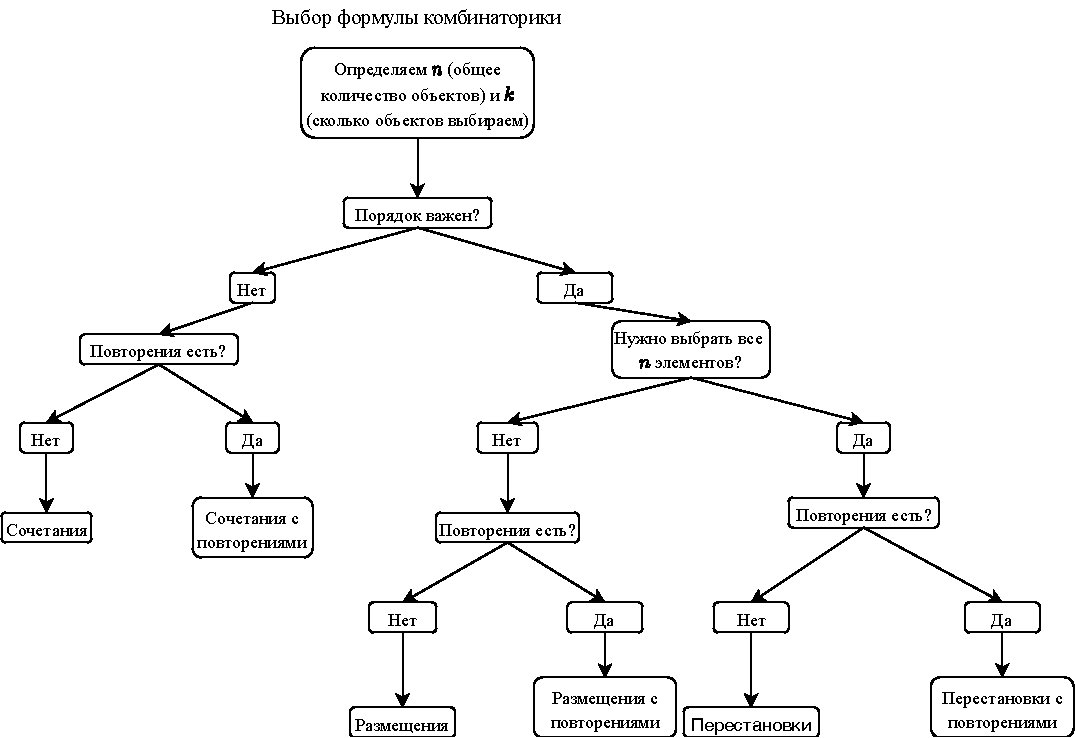
\includegraphics[]{./media/Combination_formula_choice.pdf}}
\end{figure}

\subsection{Обобщённые примеры задач}

\textbf{Задача 1.}

Пусть у нас имеется $n$ различных предметов и $k$ ящиков. Тогда каждый предмет можно положить в любой из $k$ ящиков. Следовательно получаем, что всего имеется:
\[ \underbrace{k \cdot \dots \cdot k}_{n \text{ раз}} = k^n \]
способов разместить $n$ предметов (с повторениям) по $k$ ящикам.

\textbf{Задача 2.}

Размещение предметов по ящикам при условии, что каждый ящик содержит ровно один предмет.

Первый предмет можно положить в любой из $k$ ящиков, второй - в любой из оставшихся $k-1$ ящиков, третий - в один из оставшихся $k-2$ ящиков, $\dots$, последний - в любой из оставшихся $k-n+1$. Поэтому:
\[ \dfrac{k!}{(k-n)!} \]
способов разместить $n$ предметов по $k$ ящикам по одному.

\section{Основные понятия теории вероятностей}

\begin{definition}[Событие (неформальное определение)]
	\textit{Событием} в теории вероятностей (случайным событием, возможным событием) называется любой факт, который в результате испытания, эксперимента, опыта может произойти или не произойти. Подчеркнём, что \textit{случайное событие} — это такое событие, наступление которого мы не можем в точности предвидеть из-за незнания причин, вызывающих его, или невозможности считаться со всеми причинами, или событие, которое не обязательно происходит (то есть не является детерминированным).
	
	Будем говорить, что результат эксперимента является \textit{случайным событием}, если выполнены два условия:
	\begin{enumerate}
		\item возможно многократное повторение эксперимента (мысленное или реальное, во времени или в пространстве);
		\item при каждом повторении непредсказуемым образом реализуется один
		исход из заранее известного множества всех возможных результатов эксперимента.
	\end{enumerate}
\end{definition}
\begin{remark}
	\textit{Не любое утверждение относительно какой-то математической модели может являться событием}.
\end{remark}

\begin{exmp}[События]
	Следующие эксперименты иллюстрируют понятие события:
	\begin{itemize}
		\item попадание в цель при выстреле из орудия (опыт — произведение выстрела; событие — попадание в цель);
		\item выпадение двух гербов при трёхкратном бросании монеты (опыт — трёхкратное бросание монеты; событие — выпадение двух гербов);
		\item появление ошибки измерения в заданных пределах при измерении дальности до цели (опыт — измерение дальности; событие — ошибка измерения).
	\end{itemize}
\end{exmp}

Событие называется \textbf{достоверным}, если оно обязательно произойдет в условиях данного опыта.

Событие называется \textbf{невозможным}, если оно не может произойти в условиях данного опыта. Например, событие, заключающееся в том, что из партии стандартных деталей будет взята стандартная деталь, является достоверным, а нестандартная — невозможным.

Событие называется \textbf{возможным}, или \textbf{случайным}, если в результате опыта оно может появиться, но может и не появиться. Примером случайного события может служить выявление дефектов изделия при контроле партии готовой продукции, несоответствие размера обрабатываемого изделия заданному, отказ одного из звеньев автоматизированной системы управления.

События называются \textbf{равновозможными}, если по условиям испытания ни одно из этих событий не является объективно более возможным, чем другие. Например, пусть магазину поставляют электро лампочки (причем в равных количествах) несколько заводов-изготовителей. События, состоящие в покупке лампочки любого из этих заводов, равновозможны.

\subsection{Вероятностный эксперимент. Аксиоматика Колмогорова.}

\begin{definition}[Детерминированный эксперимент]
	\textit{Детерминированные эксперименты} – это такие эксперименты, результаты которых можно предвидеть заранее на основании естественнонаучных законов, исходя из комплекса условий. Примерами детерминированных процессов являются все процессы, основанные на использовании законов классической механики, согласно с которыми движение тела однозначно определяется заданными начальными условиями и силами, которые действуют на тело.
\end{definition}

\begin{definition}[Вероятностный эксперимент]
	\textit{Вероятностный эксперимент} - это тройка $(\Omega, \Event, P)$, где
	\begin{itemize}
		\item $\Omega$ - пространство элементарных исходов - произвольное непустое множество, содержащее все возможные результаты данного случайного эксперимента, из которых в результате эксперимента происходит ровно один. Элементы этого множества называются элементарными событиями, \textit{исходами} или точками.
		\item $\Event$ - $\sigma$-алгебра подмножеств $\Omega$, называемых (случайными) \textit{событиями}. Подробнее про сигма-алгебры в разделе \ref{sigma};
		\item $P$ - вероятностная мера или \textit{вероятность}, то есть сигма-аддитивная конечная мера, такая что $P(\Omega) = 1$. Определение данных терминов будет дано позднее. Пока будем определять $P$ как неотрицательную числовую функцию такую, что $\sum\limits_{\omega \in \Omega} P(\omega) = 1$ (говорят также, что функция $P$ задает на $\Omega$ распределение вероятностей).
	\end{itemize}
\end{definition}

\begin{remark}
	Результат случайного явления описывается \textbf{исходом}, обозначаемым $\omega$. Он не наблюдается сам по себе, и в ходе случайного эксперимента, из всего мн-ва происходит ровно один.
\end{remark}

\begin{definition}[Случайное событие]
	Если $A \in \Event$, то $A \subset \Omega$, и будем называть $A$ \textit{случайным} событием. Если множество элементарных событий $\Omega$ конечное или счётное, то в качестве $\sigma$-алгебры $\Event$ берут чаще всего множество всех подмножеств (если $n$ элементов в $\Omega$, то в $\sigma$-алгебре $2^n$ событий).
	
	Над событиями определены операции теории множеств.
	
	\begin{itemize}
		\item Пересечение (логическая связка И): $A \cap B \eq$ произошло и событие $A$, и событие $B$.
		\item Объединение (логическая связка ИЛИ): $A \cup B \eq$ произошло событие $A$ или событие $B$ (могут произойти оба).
		\item Разность: $A \backslash B$ - каждый элемент принадлежит $A$ и не принадлежит $B \eq$ произошло событие $A$, но не событие $B$.
		\item $\bar A = \Omega \backslash A$ - событие, обратное к событию $A$
	\end{itemize}

	Будем говорить, что событие $A$ \textit{произошло}, если эксперимент заканчивается исходом $\omega \in A$, а если $\omega \notin A$, то событие $A$ не произошло.
\end{definition}

\begin{axioms}[множества событий]\leavevmode \vspace*{-\bigskipamount}\vspace*{-\medskipamount}
	\begin{enumerate}
		\item \textbf{АС1:} $\emptyset \in \Event$ - "ничего"\ является событием, $\Omega \in \Event$ - "всё"\ является событием. Эти события тривиальные.
		\item \textbf{АС2:} $A, B \in F \Rightarrow A \cup B \in F, A \backslash B \in \Event$
		\item \textbf{АС3:} $A_1, A_2, \dots, A_\infty \in F \Rightarrow \bigcup\limits_{i=1}^{\infty} A_i \in \Event$
	\end{enumerate}
\end{axioms}

\begin{definition}[Вероятность (Аксиоматика Колмогорова)]
	Аксиоматика Колмогорова - общепринятая аксиоматика\footnote{аксиоматика - результат строгой формализации теории, предполагающей полную абстракцию от смысла слов используемого языка, причём все условия, регулирующие употребление этих слов в теории, явно высказаны посредством аксиом и правил, позволяющих вывести одну фразу из других.} для математического описания теории вероятностей. То есть вероятность полностью определяется следующими аксиомами.
	\begin{axioms}[вероятности]\leavevmode \vspace*{-\bigskipamount}\vspace*{-\medskipamount}
		\begin{enumerate}
			\item \textbf{АВ1:} $P(\Omega) = 1$
			\item \textbf{АВ2:} Пусть есть два события $A, B \in F$, т.ч. (таких, что) $A \cap B = \emptyset$, то вероятность их объединения: $P(A \cup B) = P(A) + P(B)$ - аддитивность.
			\item \textbf{АВ3:} если $A_1, A_2, \dots \in F \text{ и } A_i \cap A_j = \emptyset, i \ne j$, то $P \left(\bigcup\limits_{i=1}^{\infty}A_i \right) = \sum\limits_{i=1}^{n}P(A_i)$ - счётная аддитивность.
		\end{enumerate}
	\end{axioms}
\end{definition}

Дадим несколько пояснений к аксиоматическому определению вероятности:
\begin{enumerate}
	\item Вероятность - это функция, действующая из множества событий в $[0,1]$.
	\[ P: \Event \to [0,1] \]
	Вероятность события $\in [0,1]$. Данная функция должна удовлетворять АВ1-АВ3!
	\item Вероятность - неотрицательная счётное-аддитивная ф-ия событий, т.ч $P(\Omega) = 1$.
\end{enumerate}
\begin{remark}
	Вероятность есть у событий, но не у исходов!
\end{remark}
\begin{remark}
	\textbf{Аксиомы Колмогорова} - аксиомы вероятностей + аксиомы событий.
\end{remark}

\subsection{Классическая схема, классическое определение вероятностей}

\textbf{Классическая схема:}
\begin{enumerate}
	\item множество исходов конечно: $|\Omega| < \infty, \Omega = \{\omega_1,\dots,\omega_n\}$;
	\item События $\Event$ - любые подмножества мн-ва $\Omega$, т.е. содержит полный набор из $2^n$ событий;
	\item Предполагаем, что все исходы равновозможны, т.е. $P(\{\omega_1\}) = P(\{\omega_2\}) = \dots = P(\{\omega_n\}) = \frac{1}{n}$.
\end{enumerate}
Рассмотрим произвольное событие $A = \{\omega_{i_1},\omega_{i_2}, \dots, \omega_{i_k}\}$ тогда
$P(A) = \dfrac{\#A}{\#\Omega}=\dfrac{k}{n}=\dfrac{\text{число исх., благопр. } A}{\text{общее число событий}}$, где $\#$ - число элементов множества.

\begin{proof}
	Исходные данные для построения требуют, чтобы  каждый элементарный исход имел одинаковую вероятность. Естественно потребовать, чтобы любое подмножество элементарных исходов было событием. Так как элементарные исходы образуют полную группу событий, то сумма их вероятностей должна быть равна 1, и из-за того, что все вероятности одинаковы, а количество  элементарных исходов равно $\# \Omega$ имеем $P(\{\omega\}) = \frac{1}{\# \Omega}$. Тогда для произвольного события $A$, используя конечную аддитивность вероятности получаем $P(A) = \frac{\# A}{\# \Omega}$. Нетрудно проверить, что так определенная функция $P$ будет вероятностью (см. определение), и что требованиям модели удовлетворяет только одна такая функция. Следовательно, математическая модель определена однозначно.
\end{proof}

\begin{remark}
	Нетрудно заметить, что классическая схема представляет собой вероятностный эксперимент, т.к. содержит в себе необходимую 3-ку элементов.
	\begin{itemize}
		\item $\Omega$ - пространство элементарных исходов. По условию оно непустое и конечное. $\surd$
		\item $\Event$ - сигма алгеброй в данном случае является набор всех подмножеств пространства элементарных исходов – это наибольшая сигма-алгебра, возможная на данном пространстве элементарных исходов. $\surd$
		\item $P$ - вероятностная мера действительно удовлетворяет условию $P(\Omega) = 1$ в связи с накладываемым условием о равновероятности событий, т.е. $\sum\limits_{i=1}^n \frac{1}{n} = 1$. $\surd$
	\end{itemize}
\end{remark}

\begin{definition}[Элементарное событие]
	Элементарное событие - это подмножество пространства исходов случайного эксперимента, которое состоит только из одного элемента. Важно заметить, что элементарное событие – это всё ещё множество, состоящее из одного элемента пространства исходов, но не сам элемент.
	Элементарное событие $\{\omega_i\}$ - неделимое. Элементарные события не пересекаются.
\end{definition}

\begin{definition}[Равновозможность]
	\[ P(\{\omega_1\}) = \dots = P(\{\omega_n\}) \]
	\[ P(\underbrace{\bigcup_{i=1}^{n}\{\omega_i\}}_{\Omega}) = \sum_{i=1}^{n} P(\{\omega_i\}) = n P(\{\omega_i\}) = 1 \text{ по АВ 1} \]
\end{definition}

\[ P(\{\omega_i\}) = \dfrac{1}{n} \]

\begin{exmp}[Бросание монеты]
	\[ \Omega = \{ \text{'О'}, \text{'Р'} \} \]
	
	События друго вида выпадают из классической схемы, потому что мы не можем оценить их вероятности, они разной природы с событиями выпадениям орла или решки.
	
	\[ \Event = \{ \emptyset, \{O\}, \{P\}, \Omega \} \]
	\[ P(\emptyset) = 0, ~~~ P(\{O\}) = P(\{P\}) = \frac{1}{2}, ~~~ P(\Omega) = 1 \]
\end{exmp}

\begin{exmp}[Бросание двух монет]
	\[ \omega = (i_1, i_2), i_1 \in \{O, P\}, i_2 \in \{O, P\} \]
	\[ \Omega = \{ (O, O), (O, P), (P, O), (P, P) \} \]
	\[ P(\{O, O\}) = \dots = P(\{P, P\}) = \frac{1}{4} \]
	
	$P(\text{хотя бы один орёл}) = \frac{3}{4}$
\end{exmp}

\begin{exmp}[Кубик]
	\[ \Omega = \{ \omega_1, \dots, \omega_6 \} \]
	$\omega_i$ - выпала верхняя грань указанного числа, $i$ очков.
	
	$A$ - чёт. $P(A) = \dfrac{P(\{\omega_2 \omega_4 \omega_6\})}{6} = \dfrac{1}{2}$
\end{exmp}

\begin{exmp}[Два кубика]
	$A$ - сумма очков равна 9.
	
	Рассмотрим 3 вероятностные модели:
	
	\[ \tilde{\omega_i} - \text{сумма очков равна } i \]
	\[ \tilde{\omega_{ij}} - \text{на одном кубике } i \text{ очков}, \text{на другом } j \text{ очков} \]
	\[ \text{Считаем, что один кубик первый, а другой второй, и на первом } i \text{-очки, на втором - } j\text{-очки} : \omega_{ij}. \]
	Схема 1 (исход - это сумма очков):
	\[ \# \Omega = 11 \]
	\[ A = \{\tilde{\omega_i}\}, P(A) = \frac{1}{11} \]
	Схема 2 (исход - на одном $i$ очков, на другом $j$ очков):
	\[
	\begin{pmatrix}
		11    & 12   & 13 & \dots & 16 \\
		\dots & 22   & 23 & \hdotsfor{2} \\
		\hdotsfor{2} & 33 & \hdotsfor{2} \\
		\hdotsfor{3} & \ddots & \dots
	\end{pmatrix}
	\]
	\[\# \Omega = 21 ~~~~~~~~~ A = \{ \bar \omega_{36}, \bar \omega_{45} \} \]
	\[ P(A) = \frac{2}{21} \]
	Схема 3 (исход - на первом $i$ очков, на втором $j$ очков):
	\[ \Omega = 36 ~~~~~~~~~ A = \{ \omega_{36}, \omega_{45}, \omega_{54}, \omega_{63} \} \]
	\[ P(A) = \frac{4}{36} = \frac{1}{9} \]
	
	Все решения верны, но не все подходят для модели. В первом решении, очевидно, нет равновозможности элементарных событий
	
	Рассмотрим событие $\{\bar \omega_{55}\} \eq \{\omega_{55}\}$ и событие $\{\bar \omega_{36}\} \eq \{\omega_{36}, \omega_{63}\}$. Они неравновозможны.
	
	В схеме 3 события инвариантны, в остальных - нет.
\end{exmp}

\subsection{Геометрическая схема, геометрическое определение вероятности}

Классическое определение вероятности неприменимо, если логически возможных исходов эксперимента бесконечно много. В качестве примера рассмотрим следующую геометрическую задачу. Пусть $\Omega$ - квадрируемое (то есть имеющее площадь) множество, $A$ - его квадрируемое подмножество. Какова вероятность, что случайно выбранная точка $M$ из $\Omega$ принадлежит также и $A$ (как говорят, "попадет в $A$"\,)? Если предположить, что вероятность попадания в произвольную квадрируемую часть $\Omega$ зависит только от площади этой части (причём прямо пропорционально) и не зависит от ее расположения в $\Omega$, то естественно за эту вероятность принять, по определению, отношение площадей:
\[ P(A) = \frac{\text{площадь}(A)}{\text{площадь}(\Omega)} \]

Это определение хорошо согласуется с классическим. Действительно, если множество $\Omega$ разбито на $n$ частей равной площади, то вероятность попадания случайной точки в каждую такую часть по обоим определениям равна $\frac{1}{n}$.

Хорошо известно, что квадрируемые подмножества $\Omega$ образуют $\sigma$-алгебру. В силу этого можно рассматривать сигма-алгебру $\Event$ событий на $\Omega$, состоящую из всех его квадрируемых подмножеств. В них будут иметь смысл сумма, произведение, разность событий и дополнение их до $\Omega$.

Аналогичная модель $(\Omega, \Event, P)$ может быть построена при условии, что $\Omega$ - спрямляемое множество (имеющее длину) или кубируемое множество (имеющее объем).

Дадим более строгое математическое определение данному факту.

Выбираем множество $\Omega \subset\mathbb{R}^d$. Включает в себя ряд моделей $d$-размерностей. $V_d(\Omega) \in (0, \infty)$.

\begin{itemize}
	\item $d = 1, V_d$ - длина
	\item $d = 2, V_d$ - площадь
	\item $d = 3, V_d$ - объём
\end{itemize}

\[ \Event = \{ A \in \mathcal{B}_d : A \subseteq \Omega \} ~~~~~~~~~ P(A) = \frac{V_d (A)}{V_d (\Omega)} \]

\begin{definition}[Наугад брошенная точка]
	Точка, наугад брошенная в множество $G$, если вероятность попадания в подмножество $G$ не зависит от формы и местоположения, а зависит только от его объёма.
\end{definition}

Данное определение эквивалентно геометрическому определение вероятности. $P(G) = 1$, т.к. наше множество и есть всё пространство элементарных исходов ($\Omega$). Выражение же "бросается"\, наугад имеет следующий смысл: брошенная точка может попасть в любую точку области $G$, вероятность попасть в какую-либо часть точки области $G$ пропорциональна мере этой части (длине, площади, объему и т.п.) и не зависит от её расположения и формы. Уже показано, что подмножество множества $G$ образует $\sigma$-алгебру, а также на них определены операций над событиями. т.е. объединение, пересечение, дополнение событий снова дают событие. Таким образом, вероятность определяется по формуле, обозначенной для геометрической схемы выше.

\begin{exmp}
	Точка наугад бросается в $[0,1], A$ - расстояние от ближайшей границы интервала $\le \frac{1}{3}$.
	\[ \Omega = [0, 1], ~~~~~~~~~ V_1(\Omega) = 1 \]
	\[ A = \left[ 0; \frac{1}{3} \right] \cup \left[ \frac{2}{3}, 1 \right] ~~~~~~~~~ V_1 (A) = \frac{2}{3} \]
	\[ P(A) = \frac{2}{3} = \frac{V_1 (A)}{V_1 (\Omega)} \]
\end{exmp}

\begin{exmp}[Задача о встрече]
	Двое договорились о встрече в определенном месте. Каждый из них приходит в условленное место независимо друг от друга в случайный момент времени из $[0; T]$ и ожидает не более чем время $t \in (0; T)$. Какова вероятность встречи на таких условиях?
\end{exmp}
\begin{figure}[H]
	\center{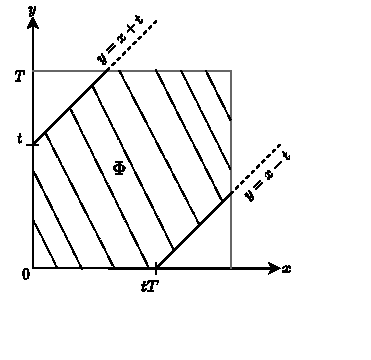
\includegraphics[scale=1.3]{./media/meet_task.pdf}}
\end{figure}
\begin{nonum}
	Обозначим через $x$ время прихода первого в условленное место, а $y$ - время прихода туда второго лица. Из условия вытекает, что $x$ и $y$ независимы друг от друга пробегают промежуток времени  $[0; T]$. Испытание состоит в фиксации времени прихода указанных лиц к месту встречи. Тогда пространство элементарных исходов данного испытания интерпретируется как совокупность всех точек $M(x; y)$ квадрата $\Omega = \{ (x; y) : 0 \le x \le T, 0 \le y \le T \}$.
	Интересующее нас событие A - "встреча произошла"\, наступает в том и только том случае, когда выбранная точка $M(x; y)$ окажется внутри фигуры $\Phi$, представляющей собой множество всех точек квадрата, координаты которых удовлетворяют неравенству $|x-y| \le t$. По формуле, представленной ниже,
	\begin{center}
		\fbox{%
			\parbox[t][5.4cm]{13cm}{%
				Формула $P(A) = \frac{m}{n}$ теряет смысл, если число всех равновозможных несовместных случаев неограничено (образует бесконечное множество). Однако возможно иногда всей совокупности бесконечных равновозможных несовместных случаев дать количественную характеристику $S$ в некоторых мерах
				длины, площади, объема, времени и так далее, а части этой совокупности, благоприятствующей наступлению рассматриваемого события $A$ - характеристику $S_{\delta}$ в тех же мерах. Тогда вероятность появления события $A$ определяется соотношением:
				\[ P(A) = \frac{S_{\delta}}{S} \]
		}}\qquad
	\end{center}
	искомая вероятность представляет собой отношение площади фигуры $\Phi$ к площади квадрата $\Omega$:
	\[ P(A) = \frac{T^2 - (T-t)^2}{T^2} = 1 - \left( 1 - \frac{t}{T} \right)^2 \]
	Анализируя полученный в этой задаче результат, видим, что с возрастанием $t \in (0; T]$ увеличивается вероятность встречи.
	
	Пусть, например, $T = 1$ час, $t = 20$ мин., тогда $P(A) = \frac{5}{9} > 0.5$, то есть чаще чем в половине случаев встречи будут происходить, если многократно договариваться на указанных выше условиях.
\end{nonum}

\subsubsection{Некорректные постановки задач}

\begin{exmp}[Парадокс Бертрана]
	Хорда наугад бросается на окружность. Найти вероятность того, что длина хорды не превышает ($\ge$) длина стороны правильного вписанного треугольника. Случайным является местоположение хорды. Если знаем середину $\Rightarrow$ знаем, где находится, т.к. она $\perp$ радиусу.
	
	Рассмотрим \textbf{первый} подход - метод "случайного радиуса"\ . Фиксируем диаметр. Местоположение хорды определяется точкой на данном диаметре. Рисуем вписанный треугольник (представим, что он повёрнут так, что одна из его сторон $\perp$ зафиксированному диаметру), длина его стороны равна $\dfrac{\sqrt{3}}{2} r$. Хорда длиннее стороны треугольника, если её центр ближе к центру, чем точка пересечения треугольника с зафиксированным радиусом. Сторона треугольника делит пополам радиус, следовательно вероятность выбрать хорду длиннее стороны треугольника. Иллюстрация данного подхода приведена на рис. \ref{img:bertrand1}. Обозначения рисунка: красные хорды — длиннее стороны треугольника, синие — короче.
	
	\begin{figure}[h]
		\center{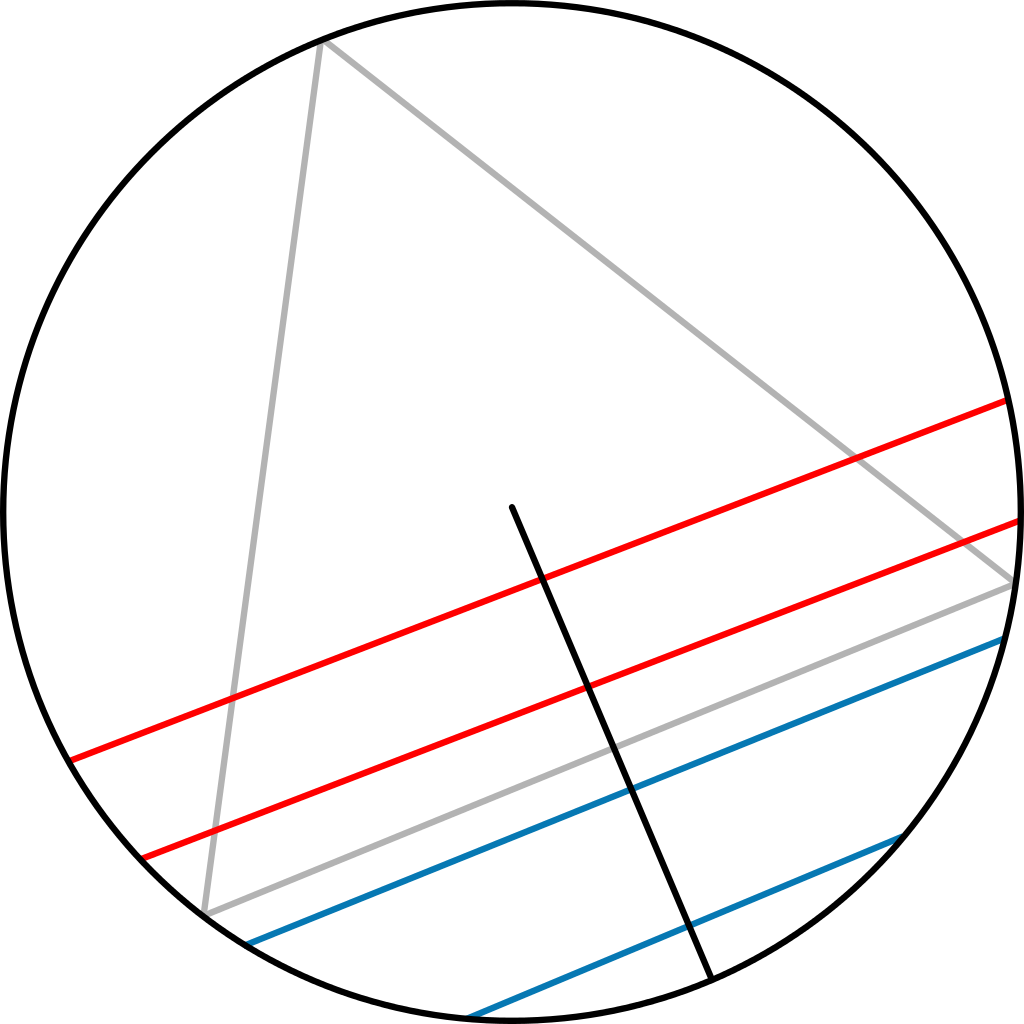
\includegraphics[scale=0.2]{./media/bertrand1.png}}
		\caption{Случайные хорды, выбранные по методу 1}
		\label{img:bertrand1}
	\end{figure}
	
	$(\cdot)$ бросания $[0, 2r]$ должна попасть в указанный отрезок. $A$ - $\{ \text{длина } x \ge \text{ длина сторон } \Delta \}$.
	\[ A - \left[\dfrac{r}{2}; \dfrac{3r}{2} \right], P(A) = \dfrac{1}{2} \]
	
	Рассмотрим \textbf{второй} подход - метод "случайных концов"\ :
	
	Наудачу выберем две точки на окружности и проведём через них хорду. Чтобы посчитать искомую вероятность, представим, что треугольник повёрнут так, что одна из его вершин совпадает с концом хорды. Заметим, что если другой конец хорды лежит на дуге между двумя другими вершинами треугольника, то длина хорды больше стороны треугольника. Длина рассмотренной дуги равна трети длины окружности. Иллюстрация данного подхода приведена на рис. \ref{img:bertrand2}.
	
	\[ \omega \in [0, \pi] - \text{угол между касательной и хордой} \]
	\[ A = [\dfrac{\pi}{3}; \dfrac{2 \pi}{3}] \Rightarrow P(A) = \dfrac{1}{3} \]
	
	\begin{figure}[h]
		\center{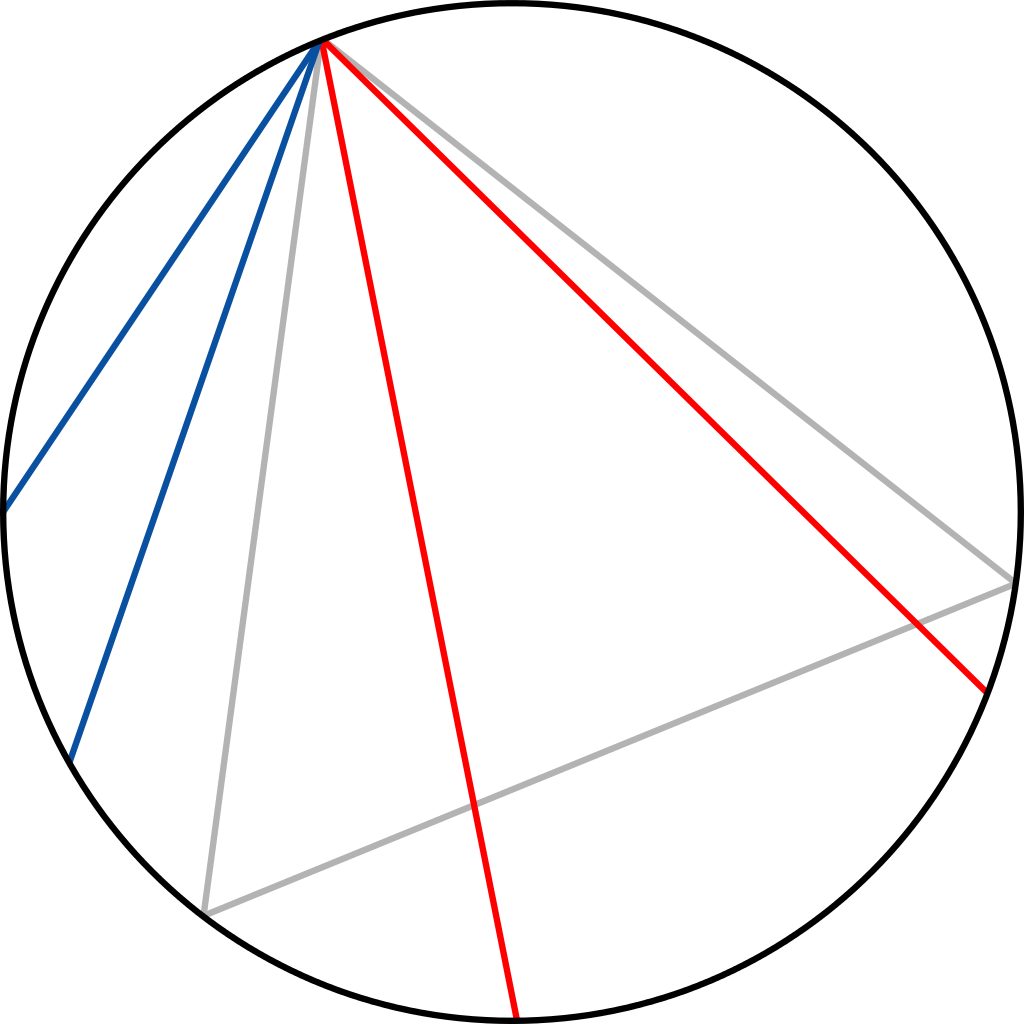
\includegraphics[scale=0.2]{./media/bertrand2.png}}
		\caption{Случайные хорды, выбранные по методу 2}
		\label{img:bertrand2}
	\end{figure}
	
	Рассмотрим \textbf{третий} подход - метод "случайного центра"\ :
	
	Выберем наудачу произвольную точку внутри круга и построим хорду с центром в выбранной точке. Хорда длиннее стороны равностороннего треугольника, если выбранная точка находится внутри круга, вписанного в треугольник. Площадь вписанного круга есть 1/4 от площади большего. Иллюстрация данного подхода приведена на рис. \ref{img:bertrand3}.
	
	$\omega$ - центр хорды, $\Omega$ - круг, $A$ - круг, радиуса $\dfrac{r}{2}$.
	
	\[ P(A) = \dfrac{S_A}{S_{\Omega}} = \dfrac{1}{4} \]
	
	\begin{figure}[h]
		\center{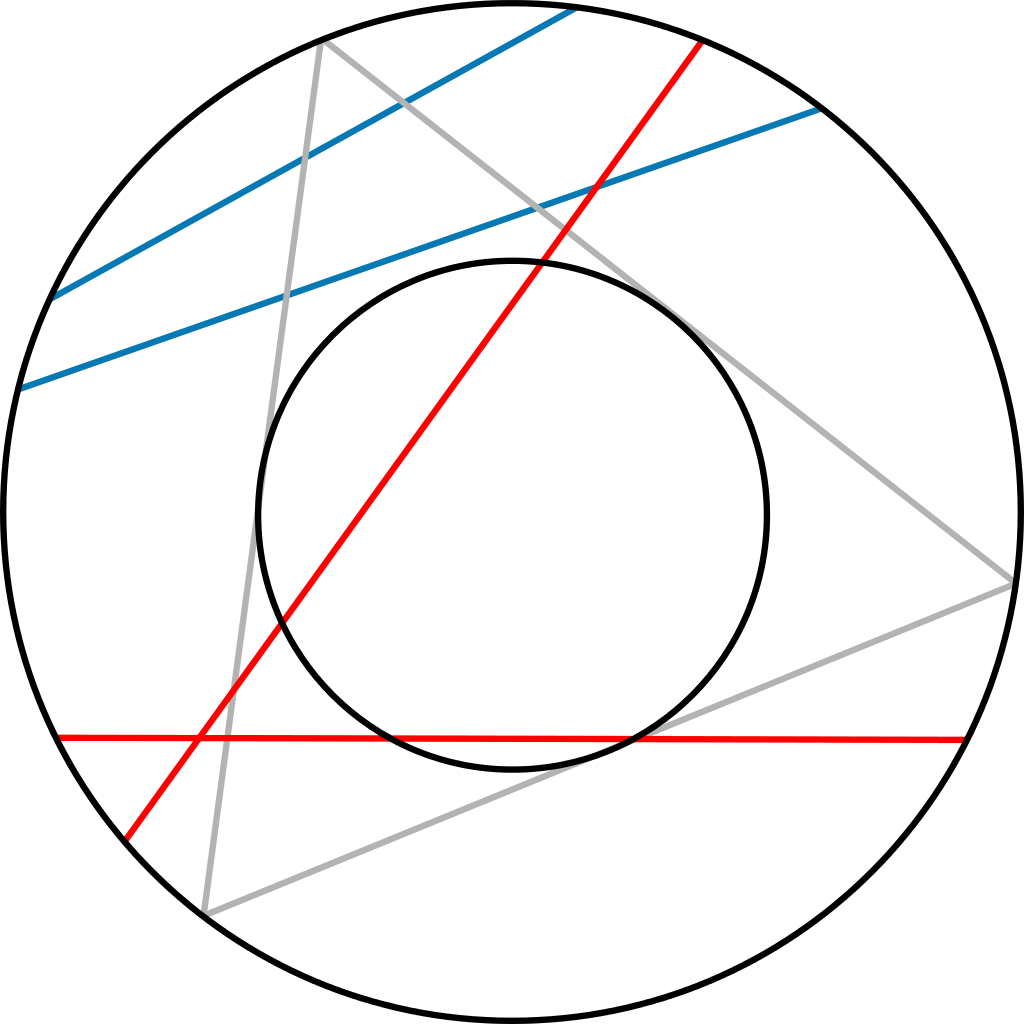
\includegraphics[scale=0.2]{./media/bertrand3.png}}
		\caption{Случайные хорды, выбранные по методу 3}
		\label{img:bertrand3}
	\end{figure}
	
	Получили 3 ответа, при этом все аргументы в док-вах корректны. Связано это с тем, что не до конца определено, что такое "бросить хорду"\ .
	
	\textbf{Классическое решение}
	
	\noindent Классическое решение проблемы, таким образом, зависит от метода, которым случайно выбрана хорда. Тогда и только тогда, когда метод случайного выбора задан, проблема имеет чётко определённое решение. Метод отбора не уникален, поэтому не может быть единственного решения. Три решения, представленные Бертраном, соответствуют различным методам отбора, и в отсутствие дополнительной информации нет оснований предпочесть какой-либо один.
	
	\textbf{Распределение местоположения центра хорды}
	
	Выбор метода также может быть изображён следующим образом. Хорда однозначно задаётся её серединой. Все три метода, описанные выше, дают различное, каждый своё, распределение середины. Методы 1 и 2 представляют два разных неравномерных распределения, в то время как третий метод даёт равномерное распределение. С другой стороны, если посмотреть на изображения хорд ниже, то заметно, что хорды в методе 2 дают равномерно закрашенный круг, а 1-й и 3-й методы не дают такой картины.
	\begin{figure}[H]
		\centering
		\subcaptionbox{Срединные точки хорд, выбранные случайным образом. Метод 1}{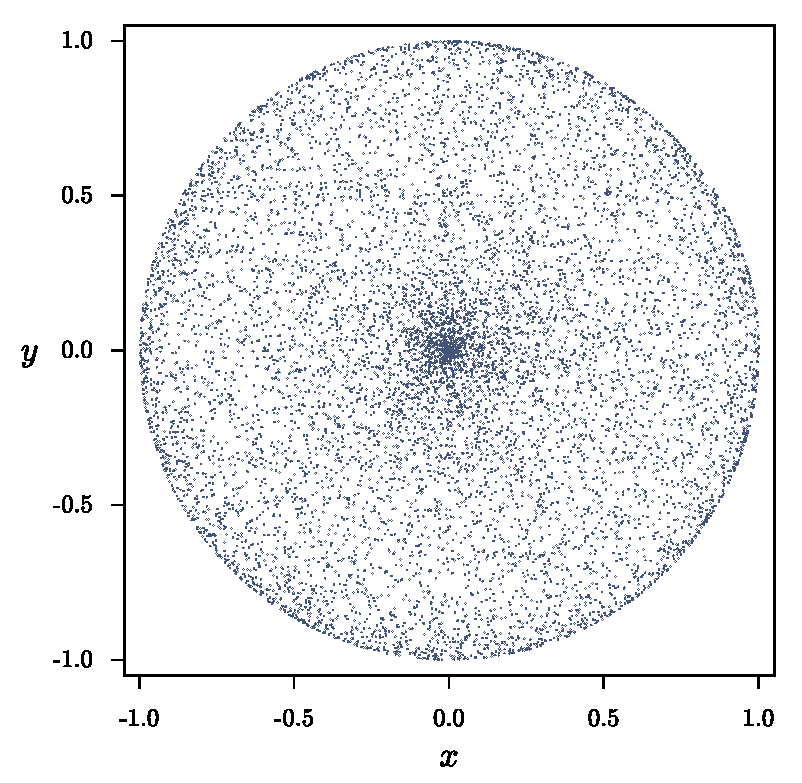
\includegraphics[width=0.25\textwidth]{./media/Bertrand1_1.pdf}}%
		\hfill
		\subcaptionbox{Срединные точки хорд, выбранные случайным образом. Метод 2}{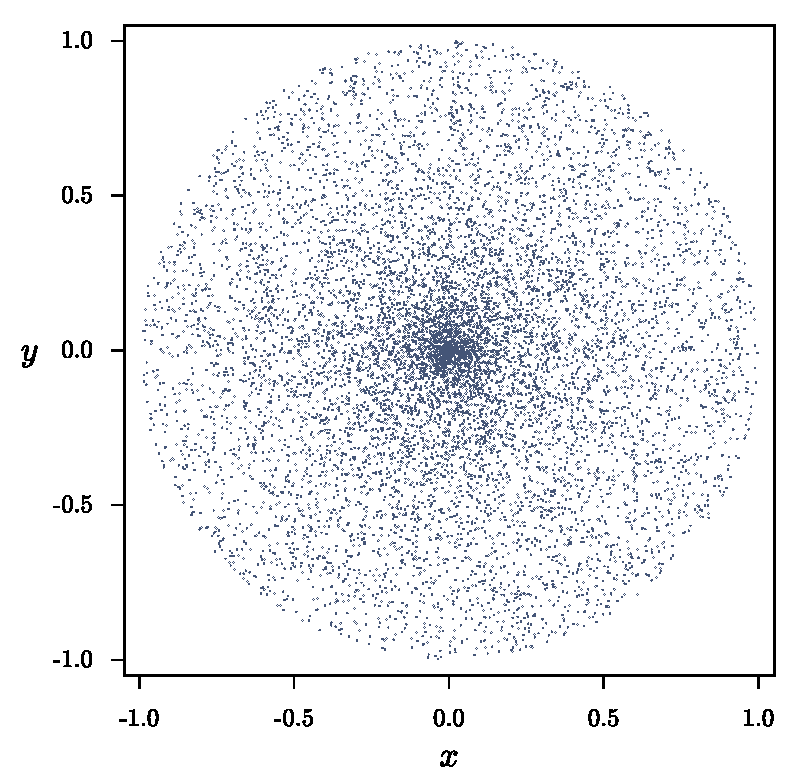
\includegraphics[width=0.25\textwidth]{./media/Bertrand2_1.pdf}}%
		\hfill
		\subcaptionbox{Срединные точки хорд, выбранные случайным образом. Метод 3}{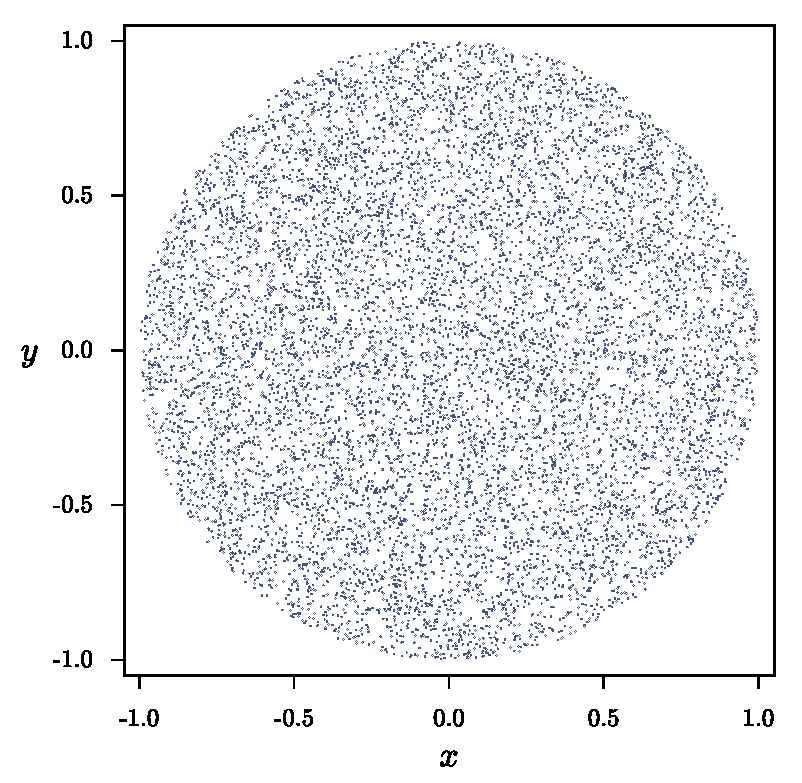
\includegraphics[width=0.25\textwidth]{./media/Bertrand3_1.pdf}}%
	\end{figure}
	\begin{figure}[H]
		\centering
		\subcaptionbox{Хорды, выбранные случайным образом. Метод 1}{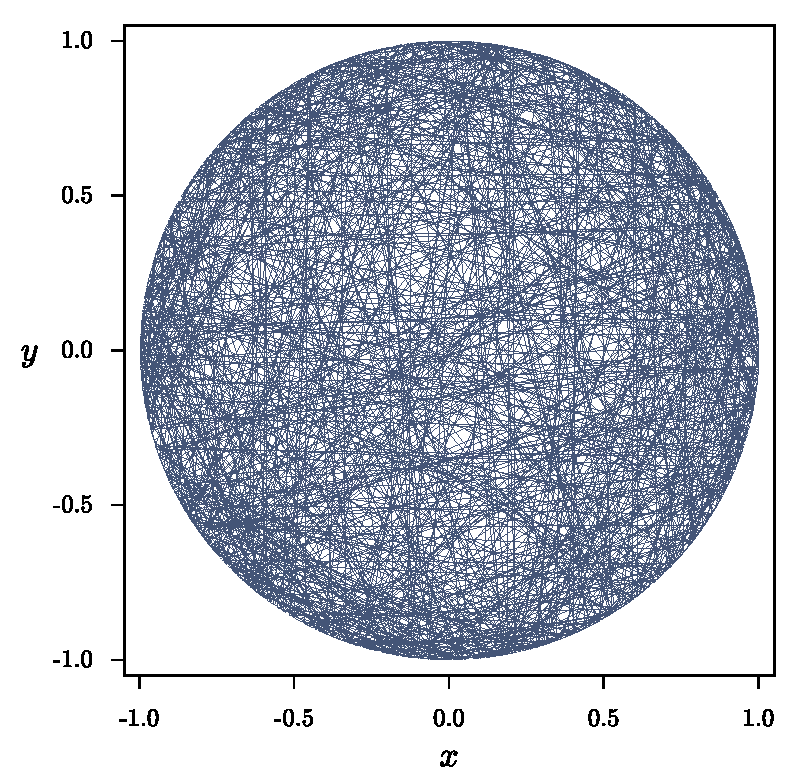
\includegraphics[width=0.25\textwidth]{./media/Bertrand1_2.pdf}}%
		\hfill
		\subcaptionbox{Хорды, выбранные случайным образом. Метод 2}{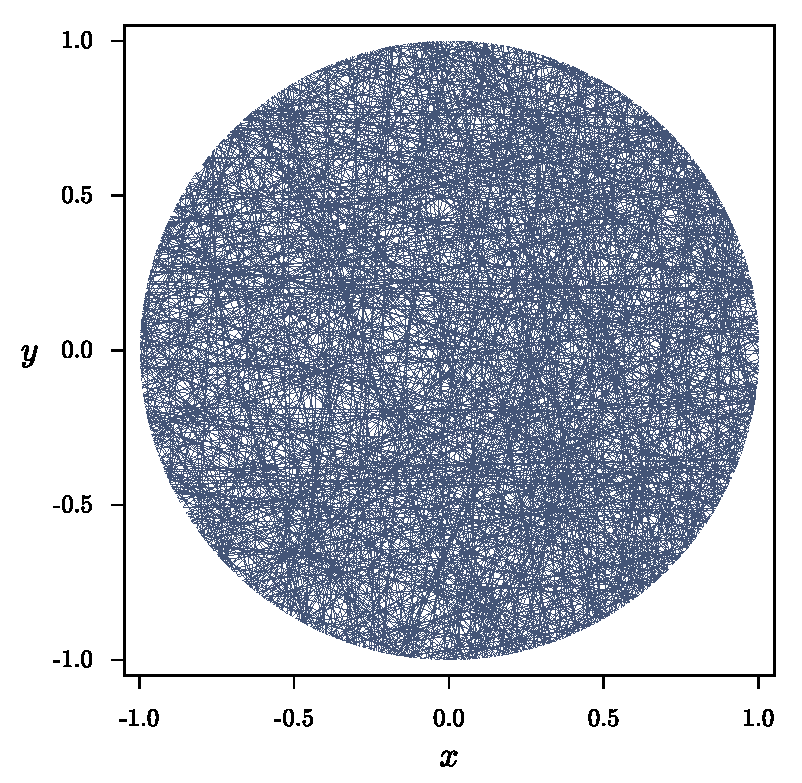
\includegraphics[width=0.25\textwidth]{./media/Bertrand2_2.pdf}}%
		\hfill
		\subcaptionbox{Хорды, выбранные случайным образом. Метод 3}{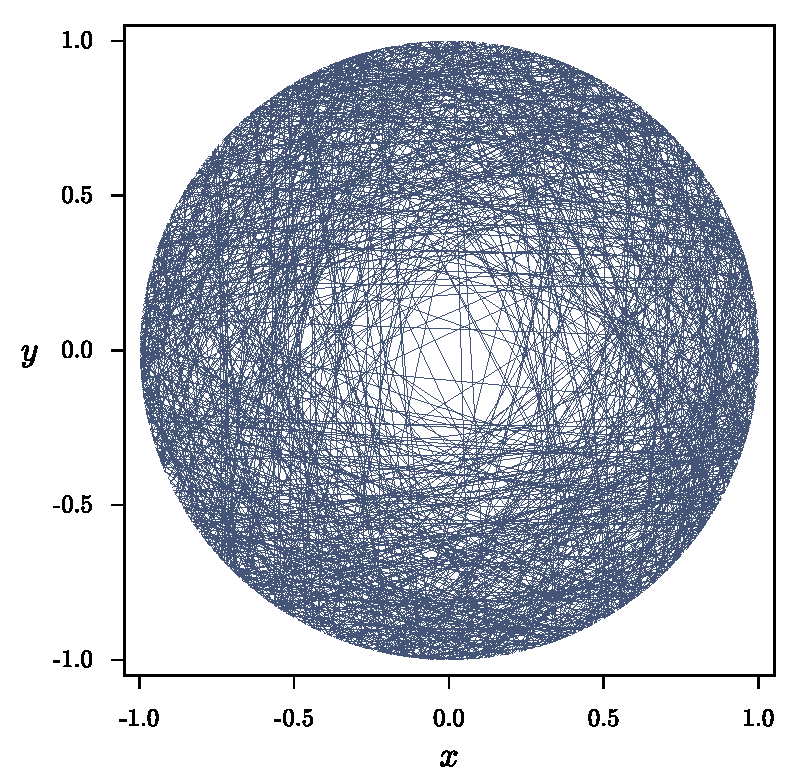
\includegraphics[width=0.25\textwidth]{./media/Bertrand3_2.pdf}}%
	\end{figure}
	Могут быть придуманы и другие распределения; многие из них дадут разные доли хорд, имеющих большую длину, чем сторона вписанного треугольника.
	
	Подробнее про распределения центра хорд можно прочитать в дополнительном разделе \ref{bertrand_paradox}.
\end{exmp}

\begin{exmp}[Бросание монеты на плоскость]
	На плоскость, разграфлённую параллельными прямыми, наугад бросается монета. Определить вероятность, что монета не пересечёт ни одну из прямых. 
	
	\noindent Радиус монеты - $r$, расстояние между прямыми - $2a, r \le a$.
	
	\noindent $\omega$ - центр монеты
	
	\begin{figure}[h]
		\center{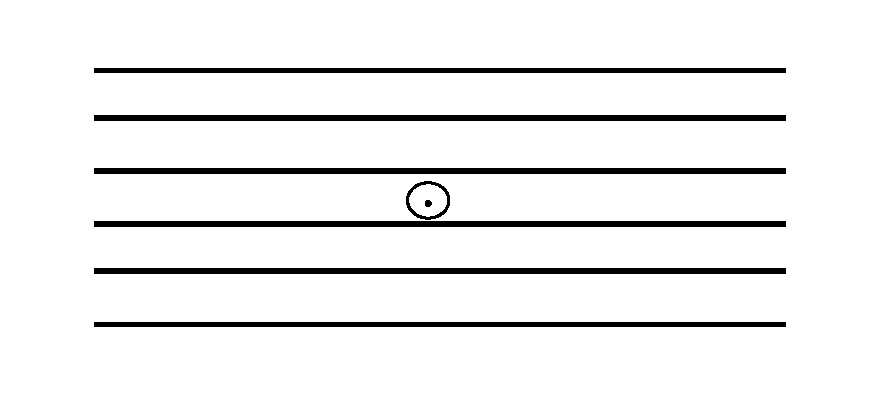
\includegraphics[scale=0.45]{./media/monetaPar.pdf}}
		\caption{Монета, брошенная на плоскость}
		\label{img:monetaPar1}
	\end{figure}

	Наугад брошенная - это значит, что вероятность попадания в множества зависит только от его, в данном случае площади. Площадь плоскости бесконечна $\Rightarrow$ для любого конечного множества  вероятность попадания в него монеты равна 0. Таким образом, монета брошена на бесконечность с вероятностью 1.
	
	Переформулируем в корректном варианте. Т.к. плоскость разделена параллельными линиям, мы можем перевести её в одну полосу и говорить, что центр монеты попал в эту полосу. Грубо говоря, мы факторизуем (накладываем) полосы друг на друга. Однако, это не спасает, т.к. площадь полосы по прежнему бесконечная, а значит и монета, брошенная на неё притянется к бесконечности. Поэтому рассмотрим просто отрезок, в который будем бросать точку - в этой формулировке уже можно решать задачу. Иллюстрация приведена на рис. \ref{img:monetaPar2}.
	
	\begin{figure}[h]
		\center{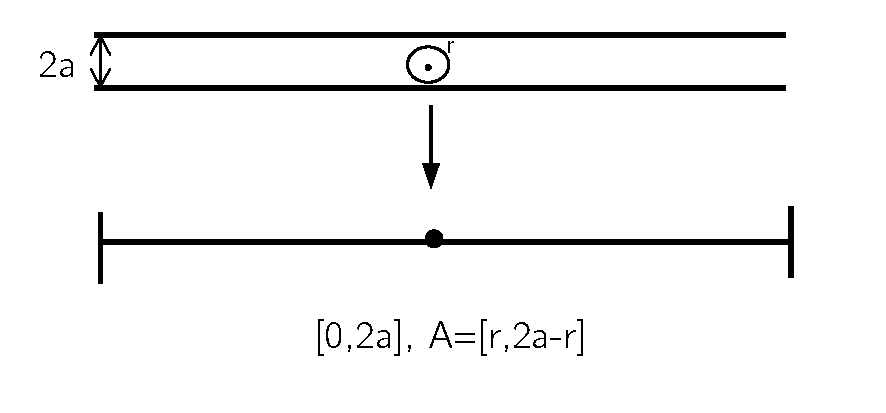
\includegraphics[scale=0.45]{./media/monetaPar2.pdf}}
		\caption{Монета, брошенная на отрезок}
		\label{img:monetaPar2}
	\end{figure}

	\[ P(A) = \dfrac{2a - 2r}{2a} = 1 - \dfrac{2}{a} \]
\end{exmp}

\subsection{Свойства вероятности}

Отталкиваемся от общей модели: пусть $(\Omega, \mathcal{F}, P)$ - вероятностный эксперимент. $A, B \in \mathcal{F}$.

\textbf{Свойства:}

\begin{enumerate}
	\item $P(\emptyset) = 0$
	\item Если определено событие $A$, то определено и обратное ему $\bar A = \Omega \backslash A$ такое, что $P(A) + P( \bar A) = 1$.
	\item $B \supseteq A \Rightarrow P(B \backslash A) = P(B) - P(A)$. 
	
	\noindent 3.' (Монотонность) $A \subset B$ (в этом случае принято говорить, что "событие $A$ предшествует событию $B$"\, или "событие $A$ влечёт за собой событие $B$"\,) $\Rightarrow P(B) \ge P(A)$. Это следует из того, что $P(A) + P(\bar A B) = P(B)$.
	
	\item $A, B \in \mathcal{F} \Rightarrow P(A \cup B) = P(A) + P(B) - P(AB) $. 
	
	\noindent 4.' $-//- \Rightarrow P(A \cup B) \le P(A) + P(B)$
	
	\item Формула включения исключения: 
	\[A_1, \dots, A_n \in \mathcal{F}: \]
	\[P \left(\bigcup_{i=1}^{n} A_i \right) = \sum_{s=1}^{n} \sum_{|\sigma| = s} (-1)^{s-1} P \left(\bigcap_{i \in \sigma} A_i \right) = \] 
	\[= P(A_1) + \dots + P(A_n) - P(A_1 A_2) - P(A_1 A_3) - \dots \pm (-1)^n P(A_1, \dots, A_n) \]
	
	\noindent $\sigma$ - сочетание индексов $\{ 1, \dots, n \}, s = |\sigma|$ - число элементов сочетания.
	\item Свойство непрерывности ($\eq$ АВ1, АВ3):
	
	$\letus$ имеется вложенный $\infty$ набор "расширяющихся"\, событий: $ A_1 \subset A_2 \subset \dots A_i \in \mathcal{F} $, тогда
	\[ \lim_{n \to \infty} P \left( \bigcup_{i=1}^{n} A_i \right) = P \left( \bigcup_{i=1}^{\infty} A_i \right) = \lim_{n \to \infty} P(A_n) \]
	
	\noindent 6.' (Комплементарное свойство) $A_1 \supset A_2 \supset \dots A_i \in \mathcal{F}$
	\[ \lim_{n \to \infty} P \left( \bigcap_{i=1}^{n} A_i \right) = \lim_{n \to \infty} P(A_1) \]
\end{enumerate}

\begin{proof}\leavevmode\vspace*{-\medskipamount}
	\begin{enumerate}
		\item $A \in \Event$ - произвольное событие.
		
		$A \cap \emptyset = \emptyset \Rightarrow \underbrace{P(A \cup \emptyset)}_{= P(A)} \stackrel{\text{АС2}}{=} P(A) + P(\emptyset) = P(A)$
		
		\item Следствие из 3-его свойства.
		
		\item $P(B) = P((B \backslash A) \cup A) \stackrel{\text{АВ2}}{=} $
		$(B \backslash A \cup A)= \emptyset$
		$= P(B \backslash A) + P(A) \Rightarrow P(B \backslash A) = P(B) - P(A)$. Дополнение в этом пункте следует отсюда же.
		
		\item $P(A \cup B) = P(A \cup \underbrace{B \backslash A}_{= B \backslash AB}) = P(A) + P(B \backslash (AB)) = \stackrel{\text{3 пункт}}{=} P(A) + P(B) - P(AB)$
		
		\item По индукции
		
		\item $A_n = \bigcup_{i=1}^n A_i = \underset{A_1}{B_1} \cup \underset{A_2 \backslash A_1}{B_2} \cup \dots \cup \underset{A_n \backslash A_{n-1}}{B_n}$
		
		\[ P(A_n) = \sum_{i = 1}^{n} P(B_i) \]
		\[ P \left(\bigcup_{i=1}^{\infty} \right) \stackrel{\text{АВ3}}{=} \sum_{i=1}^{\infty} P(B_i) = \lim_{n \to \infty} \mathbf{\sum_{i=1}^{n} P(B_i)} = \lim_{n \to \infty} P \left(\underset{= A_n}{\bigcup_{i=1}^n A_i} \right) \]
		
		\item $\bigcap_{i=1}^n A_i = \Omega \backslash \bigcup_{i=1}^n (\Omega \backslash A_i) \Rightarrow$ используем св-во 6.
	\end{enumerate}
\end{proof}

\begin{exmp}[Задача о письмах]
	$n$ писем случайным образом распределяют по $n$ конвертам. Каждый со своим адресом. Необходимо определить вероятность того, что хотябы одно письмо попадёт в свой конверт (отправится по верному адресу).
	
	\textbf{Решение:}
	
	\noindent $\omega$ - перестановка $n$ элементов (писем по конвертам)
	\[ \# \Omega = n! \]
	Событие $A_i$ - $i$-ое письмо попало в свой конверт
	\begin{figure}[H]
		\center{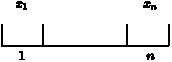
\includegraphics[scale=1.5]{./media/envelope_problem_1.pdf}}
	\end{figure}
	\[ P(A_i) = \frac{1}{n} (= P(A_1)) \]
	\[ P(A) = P \left( \bigcup\limits_{i=1}^{n} A_i \right) = \sum\limits_{s=1}^{n} (-1)^{s-1} \sum\limits_{1 \le i \dots \le i_s \le n} P(A_{i_1} \dots A_{i_s}) = \dots \]
	\[ \text{число слагаемых } = C_{n}^{s} ~~~~~~~~~~~~~ P(A_i A_j) = P(A_1 A_2) = \frac{(n-2)!}{n!} \]
	\begin{figure}[H]
		\center{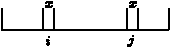
\includegraphics[scale=1.5]{./media/envelope_problem_2.pdf}}
	\end{figure}
	\[ P(A_{i_1} \dots A_{i_s}) = P(A_1 \dots A_s) = \frac{(n-s)!}{n!} \]
	\[ \dots = \sum\limits_{s=1}^{n} (-1)^{s-1} \cdot C_{n}^{s} \frac{(n-s)!}{n!} = \sum\limits_{s=1}^{n} (-1)^{s-1} \frac{n! (n-s)!}{s! (n-s)! n!} = \frac{\sum\limits_{s=1}^{n} (-1)^{s-1}}{s!} \underset{n \to \infty}{\to} 1 - e^{-1} \]
	Таким образом, ответ слабо зависит от количества писем и конвертов и примерно равен константе $\approx 0.63212$.
\end{exmp}

\subsection{Независимость двух событий. Формула полной вероятности. Формула Байеса.}

\begin{definition}[независимость 2-х событий]
	Имеется вероятностный эксперимент $(\Omega, \mathcal{F}, P)$. События $A, B \in \mathcal{F}$ независимы, если $P(AB) = P(A) P(B)$.
\end{definition}

\begin{definition}[Условная вероятность]
	Пусть $A, B$ - события, $P(B) > 0$. Условная вероятность $A$ при условии $B$: $P(A | B) = \dfrac{P(AB)}{P(B)}$
\end{definition}
\begin{remark}
	Пусть $B$ - произошло, тогда
	\[ P(B|B) = 1 ~~~~~~ P(A^*|B) = \frac{P(A^*)}{P(B)}, A^* \subset B ~~~~~~ P(A^{**} | B) = 0, A^{**} \cap B = \emptyset \]
	\[ P(\bar B | B) = 0 ~~~~~~ A = AB \cup A \backslash B ~~~~~~ P(A|B) = P(AB | B) + \underset{=0}{P(A \bar B | B)} \]
\end{remark}
\begin{figure}[h]
	\center{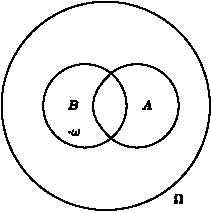
\includegraphics[scale=1]{./media/conditional_probability.pdf}}
\end{figure}
Явным примером на понимание условной вероятности является "Парадокс мальчика и девочки"\,, описанный в данной \href{https://is.gd/O9vvRh}{статье}.

\textbf{Свойства:}
\begin{enumerate}
	\item $A \cap B = \emptyset \Rightarrow P(A|B) = 0$
	\item $A \supseteq B \Rightarrow P(A|B) = \dfrac{P(A)}{P(B)}$
	\item $A, B$ - независимы, $P(A|B) = P(A)$
	\item $P_B: \mathcal{F} \to [0,1]$, т.ч. $P_B (A) = P(A|B), A \in \mathcal{F}$
	
	$P_B$ - вероятность (т.е. удовл. АВ1-АВ3)
\end{enumerate}

\begin{theorem}
	Функция $P_B$ является вероятностью.
	\begin{proof}
		Проверим три соответствующих условия, гарантирующих справедливость данного утверждения.
		\begin{enumerate}
			\item Возьмем произвольное событие $A$. Тогда $P_B(A) = \frac{P(AB)}{P(B)} \ge 0$, т.к. числитель неотрицательный, а знаменатель положительный.
			\item $P_B (\Omega) = \frac{P(\Omega B)}{P(B)} = \frac{P(B)}{P(B)} = 1$.
			\item Рассмотрим набор попарно несовместных событий (набор может быть и бесконечный):
			\[A_1, A_2, \dots; A_i A_j = \emptyset, (i \ne j) \]
			Тогда
			\[ P_B \left(\bigcup\limits_i A_i\right) = \frac{P \left( B \cap \left( \bigcup\limits_i A_i \right) \right)}{P(B)} = \frac{P \left( \bigcup\limits_i BA_i \right)}{P(B)} = \]
			\[ = \frac{\sum\limits_{i} P(BA_i)}{P(B)} = \sum_{i} \frac{P(BA_i)}{P(B)} = \sum_{i} P(A_i | B) = \sum_{i} P_B(A_i) \]
		\end{enumerate}
		Из приведенных соотношений следует, что функция $P_B$ - вероятность.
	\end{proof}
\end{theorem}

\begin{exmp}
	В колоде 52 карты / 54 карты (+2 джокера). Вытаскивают наугад 1 карту. Рассматриваются 2 варианта: $A - \{ \text{Туз} \}, B - \{ \text{Черви} \}$.
	
	$\omega$ - вытащенная карта, $\Omega = 52$.
	\[ \# A = 4, \# B = 13, \# AB = 1 \]
	\[ P(A) = \dfrac{4}{52} = \dfrac{1}{13}, P(B) = \dfrac{13}{52} = \dfrac{1}{4} ~~~~~~ P(AB) = \dfrac{1}{52} \]
	\[ P(AB) = P(A) \cdot P(B) \Rightarrow A \text{ и } B - \text{независимы} \]
	
	Теперь рассмотрим колоду с 54 картами. Ни туз, ни червовая - это не джокеры.
	
	$\omega$ - вытащенная карта, $\Omega = 54$.
	\[ \# A = 4, \# B = 13, \# AB = 1 \]
	\[ P(A) = \dfrac{4}{54} = \dfrac{2}{27}, P(B) = \dfrac{13}{54}, P(AB) = \dfrac{1}{54} \]
	\[ P(AB) \ne P(A) \cdot P(B) \Rightarrow A \text{ и } B - \text{зависимы} \]
	
	\[ P(B|A) = \dfrac{\frac{1}{54}}{\frac{4}{54}} = \dfrac{1}{4} \]
	
	Данная вероятность совпала с вероятностью в колоде с 52 картами.
	
	То, что вытащили туз - полезная информация - "это не джокер"\ . Т.е. получаем тот же вывод, что и в 1-ом варианте.
\end{exmp}

\subsection{Формула полной вероятности. Формула Байеса.}

\begin{definition}[Полная группа (система) событий]
	Пусть $ \{ H_i \}_{i=1}^n $ - некоторый набор случайных событий. Назовём его ПГС, если выполняются следующие условия:
	\begin{enumerate}
		\item $H_i \cap H_j = \emptyset$ - события попарно несовместны (не могут появится одновременно в рез-те однократного проведения эксперимента).
		\item $\bigcup\limits_{i=1}^{n} H_i = \Omega$
		\item $P(H_i) > 0, \forall i$
	\end{enumerate}
\end{definition}

\begin{remark}
	Независимость $\Rightarrow (\cancel{\Leftarrow})$ попарная независимость.
\end{remark}

\begin{definition}[Формула полной вероятности]
	Пусть $\{A_i\}_{i=1}^{n}$ - ПГС и для всех $i \ge 0$ верно нер-во $P(A_i) > 0$. Тогда для любого случайного события $B$ его вероятность можно вычислить по формуле:
	\[ P(B) = \sum_{i} P(B|A_i) P(A_i) \]
\end{definition}
\begin{remark}
	Количество элементов полной группы событий может быть и бесконечным, но обязательно счетным.
\end{remark}
\begin{proof}
	Из приведенных условий следует, что $B = \bigcup\limits_{i}A_iB$. Кроме того, события $BA_1, BA_2, \dots$ несовместны, поэтому
	\[ P(B) = P(B \cap \Omega) = P \left( B \cap \left( \bigcup\limits_{i \ge 1} A_i \right) \right) = P \left( \bigcup\limits_{i \ge 1} BA_i \right) = \sum_{i \ge 1} P(BA_i) = \]
	\[ = \sum_{i \ge 1} \frac{P(BA_i) P(A_i)}{P(A_i)} = \sum_{i \ge 1} P(B|A_i) P(A_i) \]
	\begin{figure}[H]
		\center{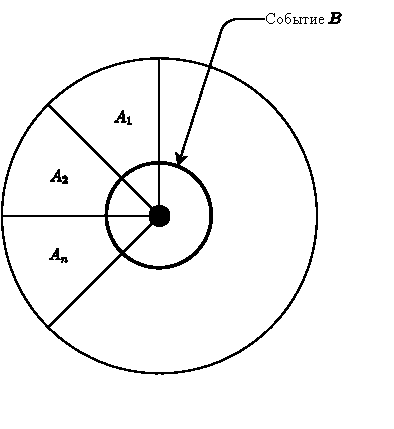
\includegraphics[scale=1]{./media/full_group_of_events.pdf}}
	\end{figure}
\end{proof}
\begin{remark}
	Формула полной вероятности верна, если просто для некоторой группы попарно несовместных событий $A_1, A_2, \dots$ будут выполняться условия: $B \subset \bigcup\limits_{i} A_i$ и $P(A_i) > 0$ для всех $i$.
\end{remark}

\begin{definition}[Формула Байеса]
	По формуле Байеса можно более точно пересчитать вероятность, беря в расчет как ранее известную информацию, так и данные новых наблюдений. Формула Байеса позволяет «переставить причину и следствие»: по известному факту события вычислить вероятность того, что оно было вызвано данной причиной. События, отражающие действие «причин», в данном случае называют гипотезами, так как они — предполагаемые события, повлекшие данное.
	
	~
	
	Дадим математическую формулировку:
	
	\noindent $\letus A \in \mathcal{F} (P(A) > 0), \{ H_i \}_{i=1}^n$ - ПГС и для всех $i \ge 1$ верно неравенство $P(H_i) > 0$. Тогда
	\[ P(H_i|A) = \frac{P(A|H_i) \cdot P(H_i)}{\sum\limits_{j=1}^{n} P(A|H_j) \cdot P(H_j)} \]
\end{definition}

Объяснения:
\begin{itemize}
	\item $\sum\limits_{j=1}^{n} P(A|H_j) \cdot P(H_j)$ - вероятность $A$, разложенная по ф-ле полной вероятности.
	\item $P(H_i)$ - априорные (судим о результатах до проведения эксперимента).
\end{itemize}

\begin{proof}
	\[ \frac{P(A|H_i)P(H_i)}{\sum\limits_{j \ge 1} P(A|H_j)P(H_j)} = \frac{P(A|H_i) P(H_i)}{P(A)} = \frac{P(H_iA)\cancel{P(H_i)}}{\cancel{P(H_i)}P(A)} = P(H_i|A) \]
\end{proof}

\begin{remark}
	Формула работает, когда есть несколько последовательных событий и последующее считать легче, что какое-то 1-ое уже произошло.
\end{remark}

Дадим небольшое словесное пояснение к формуле:
\begin{figure}[H]
	\center{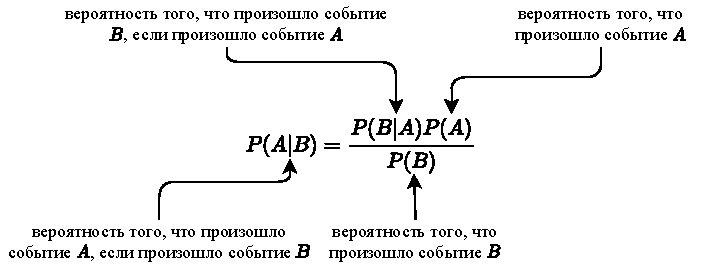
\includegraphics[scale=1]{./media/Formula_Bajesa_s_poyasneniyami.pdf}}
\end{figure}

\begin{exmp}
	Прибор может работать в одном из 2-х режимов: нормальный и экстремальный. Известно, что вер-ть выхода из строя в нормальном режиме - $0.1$, а в экстремальном - $0.8$. Известно, что прибор в реальных условиях в $90\%$ случаев работает в нормальном режиме. Определить вер-ть отказа прибора при его запуске.
	
	\textit{Решение:}
	
	Разделяем задачу на два этапа: 1-ый - в каком режиме запускает аппарат (в каком запустился, в том и работает). Событие $H_1$ - прибор запустился в нормальном режиме, $H_2$ - в экстремальном. $A$ - отказ прибора.
	
	Заполняем табличку (если не можем - решения нет):
	\begin{table}[H]
		\begin{tabular}{|c|c|c|}
			\hline
			$i$        & 1   & 2   \\ \hline
			$P(H_i)$   & 0.9 & 0.1 \\ \hline
			$P(A|H_i)$ & 0.1 & 0.8 \\ \hline
		\end{tabular}
	\end{table}

	Перемножаем по столбцам и складываем по строкам.
	\[ P(A) = 0.09 + 0.08 = 0.17 \]

	2-ой этап: определим вероятность, что прибор был запущен в экстремальном режиме. Мы знаем, что он отказал $\Rightarrow$ используем ф-лу Байеса.
	\[ P(H_2|A) = \dfrac{0.008}{0.17} = \dfrac{8}{17} \]
	
	\begin{remark}
		$P(A)$ - событие малой информации, а они несут большую информацию.
	\end{remark}
\end{exmp}

\begin{exmp}
	Автомобиль (А/м) с конвейера имеет скрытый дефект с вероятностью $0.1$. Производителя не устраивает такая большая вероятность, поэтому он проводит технический контроль. До поступления автомобиля в продажу он проходит ТК, который выявляет дефект с вероятностью $0.8$, но при этом ТК может забраковать исправный автомобиль с вероятностью - $0.1$. Определить вероятность наличия скрытого дефекта у автомобиля, купленного в магазине.
	
	\textit{Решение:}
	
	Полная группа событий - есть или нет дефект в автомобиле с завода: $H_1$ - дефект есть, $H_2$ - дефекта нет.
	
	Событие $A$ - А/м прошёл ТК.
	
	Найти нужно вероятность $P(H_1|A) - ?$
	
	\begin{table}[H]
		\begin{tabular}{ccc}
			\hline
			\multicolumn{1}{|c|}{$i$}        & \multicolumn{1}{c|}{1}         & \multicolumn{1}{c|}{2}         \\ \hline
			\multicolumn{1}{|c|}{$P(H_i)$}   & \multicolumn{1}{c|}{0.1}       & \multicolumn{1}{c|}{0.9}       \\ \hline
			\multicolumn{1}{|c|}{$P(A|H_i)$} & \multicolumn{1}{c|}{1-0.8=0.2} & \multicolumn{1}{c|}{1-0.1=0.9} \\ \hline
			& 0.02                           & 0.81                          
		\end{tabular}
	\end{table}

	\[ P(H_1|A) = \dfrac{0.02}{0.02 + 0.81} = \dfrac{2}{83} \]
\end{exmp}

\section{Независимость событий}

\begin{definition}[Независимость событий]
	Пусть $(\Omega, \mathcal{F}, P)$ - вероятностный эксперимент.
	
	События $A_1, \dots, A_n \in \mathcal{F}$ называются независимыми (в совокупности), если для любого подмножества $\forall \{ i_1, \dots, i_s \} \subseteq \{ 1, \dots, n \}, s \in [1, n]$ ($\eq$ любого сочетания индексов)
	\[ P(A_{i_1} \dots A_{i_s}) = P(A_{i_1}) \cdot ... \cdot P(A_{i_s}) \]
\end{definition}

\begin{definition}[Попарная независимость]
	События $A_1 \dots A_n$ - попарно независимы, если
	\[ P(A_iA_j) = P(A_i) \cdot P(A_j), \forall i,j: i \ne j \]
	Также данное выражение можно записать как:
	\[ P \left( \bigcap_{j = 1}^{k} A_{i_j} = \prod_{j = 1}^{k} P(A_{i_j}) \right) \]
\end{definition}

Попарная независимость не влечёт независимость, но независимость влечёт попарную независимость.

\begin{exmp}[Контр пример С.Н. Бернштейна]
	Имеется правильный тетраэдр, все грани которого — правильные треугольники, раскрашенные в один из трех цветов. Одна грань — белая, другая — красная, третья — синяя, а четвертая — пестрая, так как на ней присутствуют и белый, и синий, и красный цвета. Нас будет интересовать грань, которая при бросании тетраэдра окажется внизу, и одно из трех событий: $B, K, C$ ($B = \{ \text{на нижней грани присутсвует белый цвет} \}, K = \{ \text{на нижней грани присутсвует красный цвет} \}, C = \{ \text{на нижней грани присутсвует синий цвет} \}$). Тогда справедливы равенства: $P(B) = P(K) = P(C) = \frac{1}{2}$. Будут ли указанные события попарно независимы? Проверяем. Поскольку событие $BC$ означает, что на нижней грани присутствуют белый и синий цвета, то это означает выпадение пестрой грани. Следовательно,
	\[ P(BC) = \frac{1}{4} = \frac{1}{2} \cdot \frac{1}{2} = P(B) \cdot P(C) \]
	Так же проверяем любую другую пару и убеждаемся в попарной независимости событий $B, K$ и $C$.
	
	Независимы ли все эти три события в совокупности? Попробуем проверить. Имеем
	\[ P(BKC) = \frac{1}{4} \ne \frac{1}{2} \cdot \frac{1}{2} \cdot \frac{1}{2} = P(B) P(K) P(C), \]
	т.е. одно из необходимых равенств не выполняется. Этот пример показывает, что понятия попарной независимости и независимости в совокупности различаются.
\end{exmp}

\begin{exmp}[Второй аргумент]
	\[ P(A_1, \dots, A_n) = P(A_1) \cdot \dots \cdot P(A_n) \text{ не влечёт } A_1 \dots A_n - \text{НЗ} \]
	
	\textit{Контр пример:}
	
	\[ 0 < P(A) < 1, P(B) = 0, A_1 = A, A_2 = A, A_3 = B \]
	\[ P(A_1A_2A_3) = 0, P(A_1)P(A_2)P(A_3) = 0 \]
	\[ P(A_1A_2) = P(A) \ne P(A_1)P(A_2) = P(A)^2 \]
\end{exmp}

\begin{exmp}[Контр пример 2]
	3 раза бросается монета:
	\[ A - \{1 - 'o'\}, B - \{3 - 'p'\}, C - \{'o'>'p'\} \]
	\begin{table}[H]
		\begin{tabular}{|c|c|c|c|c|}
			\hline
			&            & A & B & C \\ \hline
			OOO & $\omega_1$ &   & * &   \\ \hline
			OOP & $\dots$    & * & * &   \\ \hline
			OPO &            & * &   & * \\ \hline
			OPP &            & * & * &   \\ \hline
			POO &            &   &   & * \\ \hline
			POP &            &   & * &   \\ \hline
			PPO &            &   &   &   \\ \hline
			PPP & $\omega_8$ &   & * &   \\ \hline
		\end{tabular}
	\end{table}

	\[ P(A) = P(B) = P(C) = \dfrac{4}{8} = \dfrac{1}{2} \]
	\[ P(AB) = \dfrac{2}{8} = \dfrac{1}{4}, P(AC) = \dfrac{3}{8} \]
	\[ P(BC) = \dfrac{1}{8}, P(ABC) = \dfrac{1}{8} \]
	\[ P(ABC) = P(A)P(B)P(C) \]
	\[ P(AB) = P(A)P(B) \]
	\[ P(AC) \ne P(A)P(C) \Rightarrow \text{ \textbf{зависимы}} \]
\end{exmp}

\begin{theorem}[Представление с использование усл. вер-ть]
	\[ A_1, \dots, A_n \in \mathcal{F} \]
	\[ P(A_1 \dots A_n) = P(A_n|A_1 \dots A_{n-1})P(A_{n-1}|A_1 \dots A_{n-2}) \dots P(A_2|A_1)P(A_1) = \]
	\[ = \left( \prod_{i=2}^{n} P(A_i|A_1 \dots A_{i-1})P(A_1) \right) \]
\end{theorem}

\section{Независимые эксперименты. Испытания Бернулли. Формула Бернулли.}

Пусть $(\Omega_1, \mathcal{F}_1, P_1), \dots, (\Omega_n, \mathcal{F}_n, P_n)$ - вероятностные эксперименты.

$\omega_1 \in \Omega_1, \dots, \omega_n \in \Omega_n$ - исходы.

Исход \textbf{комбинированного эксперимента}: $\omega = (\omega_1, \dots, \omega_n)$. 

$\Omega = \Omega_1 \times \dots \times \Omega_n$.

События $\mathcal{F} = \mathcal{F}_1 \times \dots \times \mathcal{F}_n$ - не всегда выполнено АС3. Чтобы дополнить мн-во до удовлетворения, нужно добавить всевозможные счётные пересечения: $\mathcal{F} = \sigma(\mathcal{F}_1 \times \dots \times \mathcal{F}_n)$ - мн-во включающее события.

$A_1 \times \dots \times A_n, A_i \in \mathcal{F}_i$ и их не более чем счётные $\bigcup$-я.

$P: \mathcal{F} \to [0,1]$ удовл. АВ1-АВ3.

Комбинированный эксперимент: $(\Omega, \mathcal{F}, P)$

$\Omega = \Omega_1 \times \dots \times \Omega_n$ - исходы

$\mathcal{F} = \sigma(\mathcal{F}_1 \times \dots \times \mathcal{F}_n)$ - события

$P$ - вероятность

$(\Omega, \mathcal{F}, P)$ - объединённый эксперимент

\begin{definition}[Условие согласования]
	\[ P_i(A_i) = P(\Omega \times \dots \times \Omega_{i-1} \times A_i \times \Omega_{i+1} \times \dots \times \Omega_n), \forall A_i \in \mathcal{F}_i, i = 1, \dots, n \]
\end{definition}

\begin{definition}[Независимы эксперименты]
	Эксперименты $(\Omega_1, \mathcal{F}_1, P_1), \dots, (\Omega_n, \mathcal{F}_n, P_n)$ - независимы, если $P = P_1 \times \dots \times P_n$, т.е.
	\[ P(A_1 \times \dots \times A_n) = P(A_1 \times \Omega_2 \times \dots \times \Omega_n) \cdot P(\Omega_1 \times A_2 \times \dots \times \Omega_n) \cdot ... \cdot P(\Omega_1 \times \Omega_2 \times \dots \times A_n) \]
	\[ \forall A_i \in \mathcal{F}_i, i = 1, \dots, n \]
\end{definition}

\begin{theorem}[Теорема Каратеодори о продолжении меры]
	Конечная неотрицательная счетно-аддитивная функция $\mu$ на алгебре $\mathcal{A}$ обладает единственным неотрицательным счетно-аддитивным продолжением на $\sigma$-алгебру, порождённую $\mathcal{A}$.
	
	Указанное продолжение можно задать формулой
	\[ \mu^* (A) = \inf \left\{ \sum_{n=1}^{\infty} \mu (A_n), A_n \in \mathcal{A}, A \subset \bigcup_{n=1}^{\infty} A_n \right\} \]
	Заметим, что приведенная формула имеет смысл для любого подмножества $\Omega$. Полученная функция называется внешней мерой. При этом она теряет свойство быть счетно-аддитивной на множестве всех подмножеств. Вместо этого выполнено свойство субаддитивности
	\[ \mu^* \left( \bigcup_{n=1}^{\infty} A_n \right) \ge \sum_{n=1}^{\infty} \mu^* (A_n), A_i \cap A_j = \emptyset, i \ne j \]
	Тем не менее, мера $\mu$ счетно-аддитивна даже на более широком классе множеств, чем $\sigma$-алгебра, порождённая $\mathcal{A}$.
\end{theorem}

\subsection{Испытание Бернулли. Формула Бернулли.}

\begin{definition}[Испытание]
	Испытание - эксперимент с 2-мя исходами
	\[ \Omega = \{\text{'успех'}, \text{'неудача'}\} ~~~~~~~~~~~ \mathcal{F} - \text{все п/н } \Omega \]
	\[ P(\{\text{'у'}\}) = 1 - P(\{\text{'н'}\}) = p, p \in [0,1] \]
\end{definition}

\begin{definition}[Испытание Бернулли]
	Испытание Бернулли - это совокупность $n$ независимых испытаний с одинаковой вероятностью успеха $P(\{\text{'у'}\}) = p, p \in [0,1]$.
	
	\noindent Исход $\omega = (i_1, \dots, i_n), i_j \in \{\text{'у', 'н'}\}$
	
	\noindent $\# \Omega = 2^n$, где $n$ - число испытаний Бернулли.
	
	\noindent $P(\{\omega\}) = p^k(1-p)^{n-k}, k - $ число 'у' в последовательности ($i_1, \dots, i_n$).
\end{definition}

В $n$ испытаниях Бернулли изучают:
\begin{enumerate}
	\item $\mu_n$ - число успехов в $n$ испытаниях Бернулли.
	\item $\nu_1$ - число успехов до 1-ой неудачи.
	\item $\nu_k$ - число успехов до $k$-ой неудачи.
\end{enumerate}

\begin{definition}[Формула Бернулли]
	\[ P(\mu_n = k) = C_n^kp^k(1-p)^{n-k} = C_n^k p^k q^{n-k}, k = 0,1, \dots, n \]
	
	\begin{proof}
		Элементарные события типа $\{ (\omega_1, \dots, \omega_n) \}, \omega_i \in \{ \text{'у'}, \text{'н'} \}$
		\[ \{\mu_n = k\} = \bigcup \{(\omega_1 \dots, \omega_n)\} - \text{элементарные события} \]
		$\vec{\omega}:$ число 'у' $=k$ - числу элементов $C_n^k$.
		
		$P(\{ \omega_1, \dots, \omega_n \}) = p^k (1-p)^{n-k}$, если в $(\omega_1, \dots, \omega_n)$ ровно $k$ - 'у' $(n-k)-\text{'н'}$.
		\[ P(\mu_n = k) \stackrel{\text{АВ2}}{=} \sum\limits_{\vec{\omega}} \underbrace{P(\{(\omega_1, \dots, \omega_n)\})}_{p^k(1-p)^{n-k}} = C_n^k p^k (1-p)^{n-k} \]
	\end{proof}
\end{definition}

Как ведёт себя $P_n(k)$ при фиксированных $p,n$; $P_n(k) = P(\mu_n = k)$ - ?

\[ P_n(k) \stackrel{\stackrel{<}{>}}{=} P(k+1) \mathbf{(*)} \]
\[ C_n^kp^k(a-p)^{n-k} \stackrel{\stackrel{<}{>}}{=} C_n^{k+1}p^{k+1}(1-p)^{n-k-1} \]
\[ \dfrac{n!}{k!(n-k)!}p^k(1-p)^{n-k} \stackrel{\stackrel{<}{>}}{=} \dfrac{n!}{(k+1)!(n-k-1)!}p^{k+1}(1-p)^{n-k-1} \]
\[ p \in (0,1) \]

Перепишем \textbf{(*)} $n \in 0 \div n-1$

\[ \dfrac{1}{n-k} \stackrel{\stackrel{<}{>}}{=} \dfrac{p}{k+1} \eq (1-p)(k+1) \stackrel{\stackrel{<}{>}}{=} (n-k)p \]
\[ \eq (1-p)+k \stackrel{\stackrel{<}{>}}{=} np \eq k \stackrel{\stackrel{<}{>}}{=} np - (1-p) \]

Возрастает: $k < np - (1-p)$

Убывает: $k > np - (1-p)$

Найдём наибольшее значение данной вероятности.

\begin{theorem}[Утверждение]
	а) $ P_n(k) \le P_n(k_0), \forall n $
	
	при $k_0 \in [np - (1-p), np+p]$
	
	б) $ (n+1)p \in \mathbb{N} \Rightarrow P_n(np-(1-p)) = P_n((n+1)p) $
	
	Максимум в $k_0$:
	\[ P_n(k) \le P_n(k_0) \Rightarrow \]
	\[
	\begin{cases}
		P_n(k_0 - 1) \le P_n(k_0) \\
		P_n(k_0 + 1) \le P_n(k_0) \eq P_n(k_0) \ge P_n(k_0+1)
	\end{cases} 
	\]
	\[
	\begin{cases}
		(k_0 - 1) \le np - (1-p) \\
		k_0 \ge np - (1-p)
	\end{cases}
	\begin{cases}
		k_0 \le np + p \\
		k_0 \ge np - (1-p)
	\end{cases}
	\]
\end{theorem}

\begin{theorem}[Что будет, если $n$ велико?]
	Пусть $n=1000, k = 500, p = \dfrac{1}{2}$
	\[ C_n^kp^k(1-p)^{n-k} = \dfrac{n!}{n!(n-k)!}\left( \dfrac{1}{2} \right)^{1000} \]
\end{theorem}

\section{Предельные теоремы в схеме Бернулли}

\subsection{Схема Муавра-Лапласса. Локальная предельная теорема}

\textbf{Постановка проблемы.}

Рассмотрим $n$ испытаний Бернулли. Необходимо найти величину $P_n(k)$.
\[
\begin{cases}
	n \to \infty \\
	$p$ - \text{фиксировано}
\end{cases}
\]
Например, как вычислить данную формулу для 10000-кратного подбрасывания монеты?
\[ P_{10000} (5000) = C_{10000}^{5000} \left( \frac{1}{2} \right)^{10000} \]

\textbf{Решение:}

Будем вычислять интересующую нас вероятность с некоторой погрешностью, то есть будем жертвовать абсолютной точностью. Рассмотрим $n$ испытаний Бернулли, где $p = P(\text{'у'})$ - вероятность успеха в одном испытании, $k$ - число успехов в $n$ испытаниях. Введем следующие обозначение $x_{n, k} = \frac{k - np}{\sqrt{npq}}, q = 1 - p$.

\begin{theorem}[Локальная предельная теорема Муавра—Лапласа]
	Справедливо следующее соотношение
	\[ \dfrac{P_n(k)}{\frac{1}{\sqrt{npq}} \cdot \frac{1}{\sqrt{2 \pi}} \cdot e^{- \frac{(x_{n, k})^2}{2}}} \to 1 ~~~~~~ (n \to \infty) \]
	равномерно по всем таким $k$, для которых при произвольных фиксированных $c > 0$ и $\epsilon > 0$ выполнено неравенство: $|x_{n, k}| \le c \cdot n^{\frac{1}{6} - \epsilon}$.
	
	Утверждение теоремы означает, что
	\[ P_n(k) \approx \frac{1}{\sqrt{npq}} \cdot \frac{1}{\sqrt{2 \pi}} e^{-\frac{x_{n,k}^2}{2}} = \frac{1}{\sqrt{npq}} \phi (x_{n, k}), \]
	где $\phi(x) = \frac{1}{\sqrt{2 \pi}} e^{- \frac{x^2}{2}}$ - \textit{функция Гаусса}.
	
	Для функции $\phi (x) = \frac{1}{\sqrt{2 \pi}} e^{-\frac{x^2}{2}}$ существуют таблицы, которые показывают значения функции в различных точках. Таблицы, как правило, устроены следующим образом:
	\begin{table}[H]
		\centering
		\begin{tabular}{|c|c|c|c|c|c|}
			\hline
			$x$     & $0$           & $1$           & $\dots$ & $8$           & $9$           \\ \hline
			$0, 0$  & $\phi(0, 00)$ & $\phi(0, 01)$ & $\dots$ & $\phi(0, 08)$ & $\phi(0, 09)$ \\ \hline
			$0, 1$  & $\phi(0, 10)$ & $\phi(0, 11)$ & $\dots$ & $\phi(0, 18)$ & $\phi(0, 19)$ \\ \hline
			$\dots$ & $\dots$       & $\dots$       & $\dots$ & $\dots$       & $\dots$       \\ \hline
			$1, 4$  & $\phi(1, 40)$ & $\phi(1, 41)$ & $\dots$ & $\phi(1, 48)$ & $\phi(1, 49)$ \\ \hline
			$\dots$ & $\dots$       & $\dots$       & $\dots$ & $\dots$       & $\dots$       \\ \hline
		\end{tabular}
	\end{table}
	Для того, чтобы узнать, например, значение функции $\phi$ в точке $1, 48$, надо взять значение из таблиц, стоящее на пересечении строки со значением $x = 1,4$ и столбца с цифрой 8.
	
	\begin{proof}
		В доказательстве будет использовать следующие леммы.
		\begin{lemma}[Формула Стирлинга]
			\[ n! = n^n \cdot e^{-n} \cdot \sqrt{2 \pi n} \cdot (1 + \bar o(1)) \]
		\end{lemma}
		\begin{lemma}
			Имеет место следующее разложение логарифма:
			\[ \ln (1 + x) = x - \frac{x^2}{2} + \theta x^3, \]
			где $|\theta| < 3$ для всех $|x| < \frac{1}{2}$ (остаток в форме Пиано).
		\end{lemma}
		Также для краткости изложения будем упускать упоминание индексов у величины $x_{n, k}$.
			
		Из определения величины $x_{n, k}$ имеем следующие соотношения:
		\[ k = np + x \sqrt{npq} \underset{n \to \infty}{\to} \infty ~~~~~~~~ n - k = nq - x\sqrt{npq} \underset{n \to \infty}{\to} \infty \]
		т.е.
		\[ \frac{k}{np} = 1 + x \sqrt{\frac{q}{np}} ~~~~~~~~ \frac{n - k}{nq} = 1 - x \sqrt{\frac{p}{nq}} \]
		Запишем, что такое $P_n(k)$:
		\[ P_n(k) = \frac{n!}{k! (n - k)!} \cdot p^k \cdot q^{n - k} = \]
		\[ = \frac{n^n \cdot e^{-e} \cdot \sqrt{2 \pi n} \cdot (1 + \bar o (1))}{k^k \cdot e^{-k} \cdot \sqrt{2 \pi k} \cdot (n - k)^{n-k} \cdot e^{-n+k} \cdot \sqrt{2 \pi (n - k)}} = \]
		\[ = \left( \frac{k}{np} \right)^{-k-\frac{1}{2}} \cdot \left( \frac{n - k}{nq} \right)^{-n + k - \frac{1}{2}} \cdot \frac{1}{\sqrt{2 \pi}} \cdot \frac{1}{\sqrt{npq}} \cdot (1 + \bar o(1)) \]
		Если ввести обозначение $T_{n, k} = \sqrt{npq} P_n (k)$, то получим
		\[ T_{n, k} = \sqrt{npq} P_n(k) = \left( 1 + x \sqrt{\frac{q}{np}} \right)^{-k - \frac{1}{2}} \cdot \left( 1 - x \sqrt{\frac{p}{nq}} \right)^{-n+k-\frac{1}{2}} \cdot \frac{1}{\sqrt{2 \pi}} \cdot (1 + \bar o (1)) \]
		Рассмотрим $\ln T_{n, k}$. Очевидно, что
		\[ \ln T_{n, k} = \left( -k - \frac{1}{2} \right) \cdot \ln \left( 1 + x \sqrt{\frac{q}{np}} \right) + \left( -n + k - \frac{1}{2} \right) \cdot \ln \left( 1 - x \sqrt{\frac{p}{nq}} \right) + \]
		\[ + \ln \frac{1}{\sqrt{2 \pi}} + \ln (1 + \bar o (1)) = \]
		\[ = \left( -np -x \sqrt{npq} - \frac{1}{2} \right) \left( x \sqrt{\frac{q}{np}} - \frac{x^2q}{2np} + \theta_1 \frac{x^3q \sqrt{q}}{np \sqrt{np}} \right) + \]
		\[ + \left( -nq -x \sqrt{npq} - \frac{1}{2} \right) \left( -x \sqrt{\frac{p}{nq}} - \frac{x^2p}{2nq} + \theta_2 \frac{x^3p \sqrt{p}}{nq \sqrt{nq}} \right) + \ln \frac{1}{\sqrt{2 \pi}} + \bar o (1) = \dots \]
		В силу того, что $\frac{k}{np} = 1 + x \sqrt{\frac{q}{np}} \approx 1$; $\frac{n-k}{nq} = 1 - x \sqrt{\frac{p}{nq}} \approx 1; p+q=1$ и указанных ранее свойств получаем
		\[ \dots = \frac{x^2 q}{2} - x^2q + \frac{x^2p}{2} - x^2p + \ln \frac{1}{\sqrt{2 \pi}} + \bar o (1) = - \frac{x^2}{2} + \ln \frac{1}{\sqrt{2 \pi}} + \bar o (1) \]
		Итак,
		\[ \ln T_{n,k} = - \frac{x^2}{2} + \ln \frac{1}{\sqrt{2 \pi}} + \bar o (1) \]
		Тогда
		\[ \sqrt{npq} P_n(k) = T_{n, k} = \frac{1}{\sqrt{2\ pi}} \cdot e^{-\frac{x^2}{2}} \cdot e^{\bar o (1)} \]
		Перепишем это равенство следующим образом:
		\[ \dfrac{P_n(k)}{\frac{1}{\sqrt{npq}} \cdot \frac{1}{\sqrt{2 \pi}} \cdot e^{- \frac{(x_{n, k})^2}{2}}} = e^{\bar o (1)} \underset{n \to \infty}{\to} 1 \]
	\end{proof}
\end{theorem}

\begin{exmp}
	На факультете учатся 1600 студентов и аспирантов. Какова вероятность, что ровно у 420 человек дни рождения приходятся на летний период?
	
	Будем предполагать, что все сезоны одинаковы по длительности. Тогда вероятность того, что у случайно выбранного человека день рождения отмечается летом, равна $\frac{1}{4}$. Воспользуемся локальной теоремой Муавра—Лапласа. Поскольку $x_{1600, 420} = \frac{420 - 400}{10 \sqrt{3}} = \frac{2}{\sqrt{3}}$, то
	\[ P_{1600} (420) = \frac{1}{\sqrt{1600 \cdot \frac{1}{4} \cdot \frac{3}{4}}} \cdot e^{- \left(\frac{2}{\sqrt{3}}\right)^2} \cdot \frac{1}{\sqrt{2 \pi}} = \frac{1}{10 \sqrt{3}} \cdot \phi \left( \frac{2}{\sqrt{3}} \right) \approx 0.01 \]
\end{exmp}

\subsection{Интегральная теорема Муавра-Лапласа}

\begin{theorem}
	Пусть $\xi_1, \xi_2, \dots$ - последовательность независимых одинаково распределенных случайных величин, с распределением Бернулли, то есть $P(\xi_k = 1) = 1 - P(\xi_k = 0) = p$, где $0 < p < 1$.
	
	Каждую из случайных величин $\xi_k$ можем интерпретировать как результат при $k$-ом испытании. Если случайная величина приняла значение $1$, то это означает, что в $k$-ом испытании произошел «успех», если $\xi_k$ приняла значение 0, то в $k$-ом испытании - «неудача». Тогда $\mu_n = \sum\limits_{k=1}^{n} \xi_k$ означает число «успехов» в $n$ испытаниях. Для этих случайных величин $E\xi_k = p, D\xi_k = p(1-p)$. Тогда выполнены условия теоремы Леви, и, следовательно, выполняется соотношение из ЦПТ Леви для всех $x \in \mathbb{R}$.
	
	\[ \underset{-\infty \le a < b \le \infty}{sup} \left| P_n \left( a \le \dfrac{\mu_n - np}{\sqrt{np(1 - p)}} < b \right) - \int_{a}^{b} \dfrac{1}{\sqrt{2 \pi}} e^{-\frac{t^2}{2}}dt \right| \underset{n \to \infty}{\to} 0 \]
	
	Если учесть монотонность и поведение на бесконечностях функций распределения, что приводит к окончательному выводу, фиксирующему наличие равномерной сходимости:
	
	Всё аналогично, только вместо интеграла записываем $- (\Phi (b) - \Phi (a))$.
	
	\begin{proof}
		Док-во основано на локальной теореме М-Л.
		
		\[ P \left( a \le \dfrac{\mu_n - np}{\sqrt{np(1-p)}} \le b \right) = P(np + a\sqrt{np(1-p)} \le \mu_n \le np + b\sqrt{np(1-p)}) \]
		\[ \underset{k: k \in [np+a\sqrt{np(1-p)}, np + b\sqrt{np(1-p)}]}{\sum} P(\mu_n = k) =  \]
		\[ \underbrace{\sum_{*} \dfrac{1}{\sqrt{np(1-p)}} \dfrac{1}{\sqrt{2 \pi}} e^{-\frac{((n-np)/\sqrt{np(1-p)})^2}{2}}}_{\sim \text{ сумма Римана } \int_{a}^b \frac{1}{\sqrt{2 \pi}}e^{-t^2/2}dt} + o\left(\dfrac{1}{\sqrt{n}}\right) \]
		\[ \#* = O(\sqrt{n}) \]
		\[ (x_n - x_{n-1}) = \dfrac{1}{\sqrt{np(1-p)}} \]
		\[ = \int_{a}^b \dfrac{1}{\sqrt{2 \pi}} e^{-t^2/2}dt + o(1) - \text{ равномер. на a,b в конеч. интерв.} \]
		
		\[ P(m_1 \le \mu_n \le m2) \approx \int\limits_{\frac{m_1-np}{\sqrt{np(1-p)}}}^{\frac{m_2-np}{\sqrt{np(1-p)}}} \dfrac{1}{\sqrt{2 \pi}} e^{-t^2/2}dt = \Phi \left( \dfrac{m_1-np}{\sqrt{np(1-p)}} \right) - \Phi \left( \dfrac{m_2-np}{\sqrt{np(1-p)}} \right) \]

		\[ \Phi(x) = \int\limits_{-\infty}^{x} \dfrac{1}{\sqrt{2 \pi}} e^{-t^2/2}dt = \int\limits_{-\infty}^{x} \phi (t) dt - \text{ ф-ла Лапласса} \]
		
		Иногда используется:
		\[ \Phi^*(x) = \int_{0}^{x} \dfrac{1}{\sqrt{2 \pi}} e^{-t^2/2}dt \]
		
		\[ P \left( \dfrac{\mu_n - np}{\sqrt{np(1-p)}} \in [a,b] \right) \underset{a \to - \infty, b \to \infty, n \to \infty}{\to} 0 \]
	\end{proof}
\end{theorem}

\begin{corollary}
	Если устремим $a$ к минус бесконечности, а $b$ к бесконечности, то получим равенство
	\[ \frac{1}{\sqrt{2 \pi}} \int_{-\infty}^{\infty} e^{-\frac{t^2}{2}} dt = 1 \]
\end{corollary}

\noindent \textbf{Как применять данную теорему?} Если $n$ очень большое, то
\[ P(\alpha \le k \le \beta) = P \left( \frac{\alpha - np}{\sqrt{npq}} \le \frac{k - np}{\sqrt{npq}} < \frac{\beta - np}{\sqrt{npq}} \right) \approx \]
\[ \approx \frac{1}{\sqrt{2 \pi}} \int\limits_{\frac{\alpha - np}{\sqrt{npq}}}^{\frac{\beta - np}{\sqrt{npq}}} e^{-\frac{t^2}{2}} dt = \Phi \left( \frac{\beta - np}{\sqrt{npq}} \right) - \Phi \left( \frac{\alpha - np}{\sqrt{npq}} \right), \]
где функция $\Phi (x)$ определяется следующим равенством:
\[ \Phi (x) = \frac{1}{\sqrt{2 \pi}} \int_{-\infty}^{x} e^{-\frac{t^2}{2}} dt = \int_{-\infty}^{x} \phi (t) dt \]

Некоторые простейшие свойства функции $\Phi (x)$.
\begin{enumerate}
	\item $\Phi (x) \underset{x \to \infty}{\to} 1$ и $\Phi (x) \underset{x \to - \infty}{\to} 0$
	\item $\Phi (x)$ - строго возрастающая функция.
	\item $\Phi (0) = 0.5$.
	\item $\Phi (-x) = 1 - \Phi (x)$
\end{enumerate}

\begin{exmp}
	На факультете 1600 студентов и аспирантов. Какова вероятность, что не менее, чем у 420 дни рождения приходятся на лето.
	
	Пусть $k$ - кол-во людей, у которых день рождение летом.
	\[ P_{1600} (420 \le k < \infty) \approx \Phi (x) - \Phi (1.16) \approx 0.123 \]
\end{exmp}

\subsection{Теорема Пуассона}

\begin{definition}[Схема Пуассона]
	Рассматривают последовательность серий испытаний Бернулли, где $n$ испытаний, при этом $n \to \infty$, но $\lambda = n p_n = const$. $P(\mu_n = k), k$ - не меняется с ростом $n$.
	\[ p = p_n = \dfrac{\lambda}{n}, \lambda > 0 \]
\end{definition}

\begin{definition}[Теорема Пуассона]
	В схеме Пуассона при фиксированном $k \in 0,1, \dots$
	
	\[ \left| P(\mu_n = k) - \dfrac{\lambda^k}{k!}e^{-\lambda} \right| \underset{n \to \infty}{\to} 0 ~~~~~~~~~~~~~~ \left( P(\mu_n = k)\underset{n \to \infty}{\to} \dfrac{\lambda^k}{k!}e^{- \lambda} \right) \]
	
	\begin{proof}
		\[ P(\mu_n = k) = \dfrac{n!}{k!(n-k)!} p_n^k (1-p_n)^{n-k} = \dfrac{n!}{k!(n-k)!} \left( \dfrac{\lambda}{n} \right)^k \left( a - \dfrac{\lambda}{n} \right)^{n-k} = \]
		\[ \dfrac{n(n-1) \dots (n-k+1)}{n^k k!} \lambda^k \left( 1-\dfrac{\lambda}{n} \right)^{n-n} = \]
		\[ = \dots \underset{n \to \infty}{\to} \dfrac{\lambda^k}{k!}e^{-\lambda} \]
	\end{proof}

\end{definition}

\noindent\textbf{Формула Пуассона:}

\[ P(\mu_n = k) \approx \dfrac{\lambda^k}{k!}e^{-\lambda} \]

\subsubsection{Применение ф. М-Л и Пуассона}

При большой величине $np$ - МЛ, при малом - Пуассон.

Обычно границу ставят: $np \ge 10$ и $np < 10$.

\begin{exmp}
	Монета бросается 1000 раз. Оценить вероятность:
	\begin{enumerate}
		\item[а)] $P(\mu_n = 500)$
		\item[б)] $P(490 \le \mu_n \le 510)$
		\item[в)] $\underset{min}{m} : P(500-m \le \mu_n \le 500+m) \ge 0.99$
	\end{enumerate}

	\textit{Решение:}
	
	\begin{enumerate}
		\item[а)] $P(\mu_n = 500) = \dfrac{1}{\sqrt{2 \pi} 5 \sqrt{10}} = \dfrac{1}{10\sqrt{5 \pi}}$
		\item[б)] $P(490 \le \mu_n \le 510) = \Phi \left( \dfrac{490-500}{10\sqrt{5 \pi}} \right) - \Phi \left( \dfrac{510-500}{10\sqrt{5 \pi}} \right) = 2 \Phi \left( \dfrac{1}{\sqrt{2 \pi}} \right) - 1$
		\item[в)] $\Phi \left( \dfrac{m}{10 \sqrt{5 \pi}} \right) - \Phi \left( \dfrac{-m}{10 \sqrt{5 \pi}} \right) = 2\Phi \left( \dfrac{m}{10 \sqrt{5 \pi}} \right) - 1$
		\[ \Phi(x) = 0.995 \]
		\[ \dfrac{m}{10 \sqrt{5 \pi}} \ge x \]
	\end{enumerate}
\end{exmp}

\begin{exmp}
	Вероятность сбоя при получении СМС $0.001$. За минуту поступает 2000 СМС. Определить вероятность, что будет $\le2$ сбоев.
	
	$np = \underset{=\lambda}{2} \Rightarrow$ используем схему Пуассона.
	
	\[ P(\mu_n \le 2) = P(\mu_n = 0) + P(\mu_n = 1) + P(\mu_n = 2) \stackrel{\sim}{=} \left(1 + \lambda + \dfrac{\lambda^2}{2}\right) e^{- \lambda} = 5e^{-2} \]
\end{exmp}

\section{Введение в теорию меры. Интеграл по мере.}

\subsection{Измеримое пространство. Мера.}

\begin{definition}
	$\letus ~ x$ - некоторое множество. $\mathcal{A}$ - система подмножеств множества $x$ (должны быть определены теоретико-множественные операции) такое, что:
	\begin{enumerate}
		
		$\mathcal{A}$ - \textbf{кольцо}, если:
		
		\item $\emptyset \in \mathcal{A}$
		\item $A,B \in \mathcal{A} \Rightarrow A \cup B \in \mathcal{A}$
		\item $A,B \in \mathcal{A} \Rightarrow A \backslash B \in \mathcal{A}$
		
		$\mathcal{A}$ - $\mathbf{\mathit{\sigma}}$-\textbf{кольцо}, если выполнено (1)-(3) и
		
		\item $A_1,A_2,\dots,A_i\in \mathcal{A} \Rightarrow \bigcup\limits_{i=1}^{\infty} A_i \in \mathcal{A}$
		
		$\mathcal{A}$ - \textbf{алгебра}, если выполнены (1)-(3) и
		
		\item $x \in \mathcal{A}$
		
		$\mathcal{A}-\mathbf{\mathit{\sigma}}$-\textbf{алгебра}, если (1)-(5)
	\end{enumerate}
\end{definition}

\begin{definition}[Измеримое пространство]
	$(X, \mathcal{A})$, где $\mathcal{A} - \sigma$-алгебра, называется измеримым пространством.
\end{definition}

\begin{definition}[Мера]
	Функция, действующая $\mu: \mathcal{A} \to [0, \infty]$ называется мерой.
	\begin{enumerate}
		\item[(А1)] $\forall A, B \in \mathcal{A}: A \cap B = \emptyset, \mu (A) \ge 0$
		
		$\mu (A \cup B) = \mu(A) + \mu(B)$ - аддитивность
		\item[(А2)] $\forall \{ A_i \}_{i=1}^{\infty}, A_i \in \mathcal{A} : A_i \cap A_j = \emptyset$ при $i \ne j$
		
		$\mu \left( \bigcup\limits_{i=1}^{\infty} A_i \right) = \sum\limits_{i=1}^{\infty} \mu (A_i)$ - счётная аддитивность
	\end{enumerate}
	\textbf{Мера} - неотрицательная счётно-аддитивная функция множеств из $\mathcal{A} - \sigma$-алгебра.
\end{definition}

\begin{exmp}\leavevmode \vspace*{-\bigskipamount}\vspace*{-\medskipamount}
	\begin{enumerate}
		\item \textbf{Мера Лебега.}
		
		$X = \mathbb{R}, \mathcal{A} = \mathcal{B}_1$, где $\mathcal{B}_1$ - борелевская $\sigma$-алгебра - наименьшая сигма-алгебра, содержащая все интервалы $(a, b], a, b \in \mathbb{R}, b > a$.
		
		$\mu_1$ - мера Лебега, определённая на интервалах $\mu ((a, b]) = b - a$. По свойствам меры $\mu_1$ продолжается единственным образом на $\mathcal{B}_1$.
		
		\item \textbf{Считающая мера.}
		
		$(\mathbb{R}, \mathcal{B}_1)$ - измеримое пространство.
		
		$A = \{ a_i \}_i$ - не более чем счётное множество, $B \in \mathcal{B}_1$.
		
		$\nu (B) = \# (B \cap A)$ - число элементов в $A \cap B$.
		
		\item \textbf{Вероятность.}
		
		$(\Omega, \Event)$ - измеримое пространство.
		
		$\Omega$ - множество исходов, $\Event - \sigma$-алгебра событий.
		\[ P : \Event \to [0, 1] \]
	\end{enumerate}
\end{exmp}
\textit{Примечание:}
\begin{itemize}
	\item Длина (мера на $(\mathbb{R}, \mathcal{B})$), объём (мера на $(\mathbb{R}^3, \mathcal{B}_3)$);
	
	\item Масса (мера вещ-ва в определённой области пр-ва $(\mathbb{R}^3, \mathcal{B}_3)$).
\end{itemize}

\begin{definition}[Считающая мера]
	Считающая мера $A \subseteq x, A$ - не более чем счётное
	\[ \mu_{A} (B) = \# (A \cap B), B \in \mathcal{A} \]
\end{definition}

\begin{definition}[$\sigma$-конечная мера]
	Мера $\mu - \sigma$-конечна, если $\exists \{ A_i \}_{i \in \mathbb{N}}, A_i \in \mathcal{A}$
	\[ \bigcup_{i=1}^{\infty} = x \text{ и } \mu (A_i) < \infty, i \in \mathbb{N} \]
\end{definition}

\begin{center}
	\textbf{Свойства меры}
\end{center}
\begin{enumerate}
	\item Если $\mu - \sigma$-конечна, то $\mu(\emptyset) = 0$.
	\item $B \subseteq A \Rightarrow \mu(B) \ge \mu(A)$ - монотонность и $\mu(A \backslash B) = \mu(B) - \mu(A)$
	\item $A, B \in \mathcal{A}$
	
	$\mu(A \cup B) = \mu(A) + \mu(B) - \mu(AB)$
	\item $A_1 \dots A_n \in \mathcal{A}$
	\[ \mu \left( \bigcup_{i=1}^n A_i \right) \le \sum_{i=1}^{n} \mu (A_i) \]
	\item $A_1 \dots A_n \in \mathcal{A}$
	\[ \mu \left( \bigcup_{i=1}^n A_i \right) = \sum_{s=1}^{n}(-1)^{s+1} \sum_{\sigma \subseteq \{1 \dots n\}, |\sigma|=s} \mu \left( \bigcap_{j=1}^s A_{\sigma_j} \right) \]
	\begin{remark}
		$\underset{=k}{|\sigma|}$ - число элементов множества $\sigma = (\sigma_1, \dots, \sigma_k)$
	\end{remark}
	\item $A_1 \subset A_2 \subset \dots A_j \in \mathcal{A}$
	
	\[ \mu \left( \bigcup_{j=1}^{\infty} = \lim_{j \to \infty} \mu(A_j) \right) \]
	
	$A_1 \supset A_2 \supset \dots A_j \in \mathcal{A}$
	
	\[ \mu \left( \bigcap_{j=1}^{\infty} = \lim_{j \to \infty} \mu(A_n) \right) \]
\end{enumerate}

\subsection{Интеграл Лебега}


\begin{definition}[Конечно-измеримое разбиение (КИР)]
	Пусть $(X, \mathcal{A}, \mu)$ - измеримое пространство с мерой.
	
	Набор множеств $\{ H_j \}_{j=1}^{n}$ называется конечно измеримым, если:
	\begin{enumerate}
		\item $H_j \in \mathcal{A}$
		\item $H_i \cap H_j = \emptyset, i \ne j$
		\item $\bigcup\limits_{j=1}^{\infty} H_j = X$
	\end{enumerate}
\end{definition}

\begin{definition}[Простая функция]
	Функция $f: x \to \mathbb{R}$ - простая, если $\exists \{ H_i \}_{i=1}^k$ -конечное измеримое разбиение $X$ и $\{ C_j \}_{j=1}^k$ - набор констант т.ч.
	\[ f(x) = C_i, \forall x \in H_i, i = 1, \dots, k \]
\end{definition}

\textbf{Свойства простых функций}
\begin{enumerate}
	\item $f(x) = c, \forall x \in X$ - простая
	\item $f, g$ - простые,  $\alpha, \beta \in \mathbb{R}$
	\[ \alpha f + \beta g - \text{простая} \]
	$fg$ - простая, $|f|$ - простая.
	\[ g(x) > 0, \forall x \in X \Rightarrow f/g - \text{простая} \]
	\item $\{ H_i^{(1)} \}_{i=1}^{k_1}, \{ H_j^{(2)} \}_{i=1}^{k_2} - \text{КИР}$
	\[ f(x) = C_i^{(1)}, x \in H_i^{(1)}, i = 1, \dots, k_1 \]
	\[ f(x) = C_j^{(2)}, x \in H_j^{(2)}, j = 1, \dots, k_2 \]
	Тогда
	\[ \sum_{i=1}^{k_1} C_i^{(1)} \mu (H_i^{(1)}) = \sum_{j=1}^{k_2} \mu (H_j^{(2)}) \]
\end{enumerate}

\begin{definition}[Интеграл от функции по мере]
	Пусть $f$ - простая функция по отношению к $\{ H_i \}_{i=1}^{k} - \text{КИР}$, $f(x) = C_i, x \in H_i, i = 1, \dots, k$
	Интеграл
	\[ I(f) = \int_{x} f d \mu \left( = \int_{x} f(t) \mu (dt) \right) = \sum_{i=1}^{k} C_i \mu (H_i) \]
	называется интегралом от функции $f$ по мере $\mu$.
\end{definition}
\begin{remark}
	Аналог определённого интеграла.
\end{remark}

\begin{exmp}
	Пусть $\mu = \mu_1$ - мера Лебега.
	\begin{figure}[H]
		\center{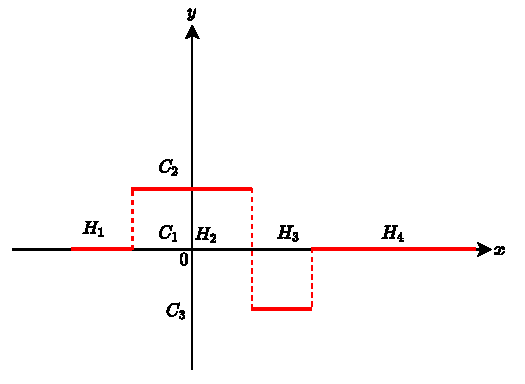
\includegraphics[scale=1]{./media/lebesgue_example.pdf}}
	\end{figure}
	\[ I(f) = C_2 \mu (H_2) + C_3 \mu (H_3) \]
\end{exmp}

\begin{definition}[Измеримая функция]
	Пусть $f: x \to \mathbb{R}$, где $(x, \mathcal{A})$ - измеримое пространство. $f$ - измеримая, если $\forall A \in \mathcal{B}_1 (A \subset \mathbb{R})$. Здесь $\mathcal{B}_1$ - борелевские множества, их $\cup$ и $\cap$ не более чем счётные.
	\[ \{ x\in X: f(x) \in A \} (= f^{-1} (A)) \in \mu \]
\end{definition}

\textbf{Свойства измеримых функций}
\begin{enumerate}
	\item $f(x) = const$ - измерима
	\item $f,g$ - измерима, $\alpha, \beta \in \mathbb{R}$
	\[ \alpha f + \beta g; \alpha f - \beta g; fg; f \backslash g; g > 0; |f|; f_{+}; f_{-} - \text{измеримые} \]
	\item $\{ f_n \}_{n \in \mathbb{N}}$ - последовательность измеримых
	\[ \lim_{n \to \infty} f_n (x) = f(x), \forall x \in X \Rightarrow f - \text{ измеримая} \]
\end{enumerate}

\begin{exmp}
	$(\mathbb{R}, \mathcal{B}_1, \mu_1); f : \mathbb{R} \to \{ -1, 0, 1 \}; f(x) = sign (x)$ - простая, т.к. принимает конечное число значений:
	\[ H_1 = \{ \dots, -2, -1 \}; ~~~ H_2 = \{ 0 \}; ~~~ H_3 = \{ 1, 2, \dots \} \]
	\[ C-1 = -1; ~~~ C_2 = 0; ~~~ C_3 = 1 \]
	\[ j = 1,2,3 : \forall x \in H_j : f(x) = C_j \]
\end{exmp}

\begin{definition}[Утверждение]
	Пусть $f$ - измерима, $f(x) \ge 0, \forall x \in X$.
	
	\noindent Тогда $\exists \{ \omega_n \}_{n=1}^{\infty}, \omega_n - \text{простая}$,
	
	\noindent $0 \le \omega_1(x) \le \omega_2(x) \le \dots , \forall x \in X$
	
	\noindent т.ч. $\lim_{n \to \infty} \omega_i(x) = f(x)$
\end{definition}

\begin{definition}[Интеграл от неотрицательной функции]
	$\letus f$ - измеримая, $f(x) \ge 0, \{ \omega_i \}_{i=1}^n$ - монотонно возрастающая последовательность простых функций
	\[ \lim_{i \to \infty} \omega_i = f(x), x \in X \]
	
	Интеграл
	\[ \int_{x} f(x) d \mu (x) \left( \int_{x} f(x) \mu (dx) \right) = \lim_{i \to \infty} \int_{x} \omega_i (x) d \mu (x) \]
\end{definition}

\begin{definition}[Эквивалентное определение]
	$f$ - измерима, $f(x) \ge 0, x \in X, \sum$ - совокупность всех простых функций.
	
	Тогда 
	\[ \int_{x} f(x) d \mu(x) = \sup_{\omega \in \sum} \int_{X} \omega(x) d \mu (x) \]
\end{definition}

\begin{definition}[Интеграл от измеримой функции]
	Пусть $f$ - измерима, $f_+ = \max (f, 0), f_- = \max (-f, 0)$
	\[ f = f_+ - f_- \]
	$f_+, f_-$ - неотрицательные измеримые,
	\[ \int_{x} f_+ d \mu (x) < \infty \]
	или
	\[ \int_{x} f_-(x) \mu (x) < \infty \]
	Тогда интеграл 
	\[ \int_{x} f(x) d \mu(x) = \int_x f_+(x) d \mu (x) - \int_{x} f_- (x) d \mu (x) \]
\end{definition}

\noindent Пусть определён $\int$-лы
\[ \int_{x} f(x) d \mu (x) \]

\noindent Будем считать, что они конечные.

\[ \int_{x} f(x) d \mu (x) < \infty \]

\noindent Тогда

\begin{remark}
	$1_A$ - индикаторная функция множества $A$.
\end{remark}

\[ \int_{A} f(x) d \mu (x) = \int_{x} f(x) 1_A d \mu (x) \]
\[ 1_A = 
\begin{cases}
	1, x \in A \\
	0, x \notin A
\end{cases}
- \text{ индикатор}
\]
\[ A \in \mathcal{F} \Rightarrow 1_A - \text{измеримая, простая} \]

\begin{center}
	\textbf{Свойства интеграла от измеримой функции}
\end{center}

$A \in \mathcal{F}, \mu$ - мера, $f, g$ - измеримые функции.
\begin{enumerate}
	\item $\int_X c d \mu = \mu (x)$
	\item $\int_X (\alpha f + \beta g) d \mu = \alpha \int_X f d \mu + \beta \int_X g d \mu$ (линейность)
	\item $f(x) \ge g(x), \forall x \in X, ~~~ \int_X f(x) d \mu \ge \int_X g(x) d \mu$ (монотонность)
	\item Пусть $A \in \mathcal{A}, \int_A f d \mu = \int_X 1_A f d \mu$
	\[ A, B \in \mathcal{A}, A \cap B = \emptyset \Rightarrow \int_{AB} f d \mu = \int_A f d \mu + \int_B f d \mu \]
	(аддитивность)
\end{enumerate}

\subsection{Интеграл Лебега и интеграл Римана}

Интеграл Лебега - более общий, чем интеграл Римана.

В интеграле Римана происходило разбиение области определения функции на интервалы и составление интегральной суммы:
\[ \int_{a}^{b} f(x) dx = \lim_{(\{x_k\}) \to \infty} \sum_{k=0}^{n-1} (x_{k+1} - x_k) f(\tilde{x_k}) \]
\begin{figure}[H]
	\center{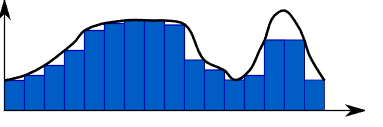
\includegraphics[scale=0.9]{./media/int_rimana.png}}
\end{figure}

В интеграле Лебега разбивается область значений функции:
\[ \int_{a}^{b} f(x) dx = \lim_{|C_{j+1} - C_{j}| \to 0} \sum_{k=0}^{n-1} C_j \mu (I_j) \]
\begin{figure}[H]
	\center{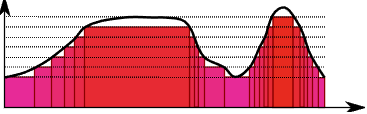
\includegraphics[scale=0.9]{./media/int_lebege.png}}
\end{figure}

\begin{exmp}
	\[
	f(x) =
	\begin{cases}
		1, & x \in \mathbb{Q} \\
		0, & x \notin \mathbb{Q}
	\end{cases}
	- \text{ функция Дирихле}
	\]
	По Риману функция не интегрируема. Однако, т.к. функция принимает только два значения, то является простой функцией и для неё определён интеграл Лебега.
	
	Рассмотрим промежуток $[0, 1]$:
	\[ \int_{[0,1]} f(x) \mu (dx) = 1 \cdot \mu \left( \mathbb{Q}_{[0,1]} \right) + 0 \cdot \mu ([0,1] \backslash \mathbb{Q}) \]
	Мера Лебега отрезка $[0,1]$ равна 1, а мера множества рациональных чисел равна 0, т.к. это множество счётно. Значит
	\[ \int_{[0,1]} f(x) \mu (dx) = 1 \cdot 0 + 0 \cdot (1 - 0) = 0 \]
\end{exmp}

\subsection{Теорема Радона-Никодима. Сингулярные и абсолютно непрерывные меры.}

Пусть $(x, \mathcal{A})$ - измеримое пространство.

\begin{definition}[Сингулярные меры]
	Меры $\mu$ и $\nu$ на $(x, \mathcal{A})$ сингулярны, если $\exists x_1, x_2 \in \mathcal{A}: x_1 \cap x_2 = \emptyset, x_1 \cup x_2 = x$, т.ч. $\mu (x_2) = 0$ и $\nu (x_1) = 0$.
\end{definition}

\begin{definition}[Абсолютно непрерывная мера]
	Мера $\mu$ абсолютно непрерывна по отношению к $\nu$ ($\mu \ll \nu, \nu - \text{ доминирует } \mu$), если $\nu(A) = 0 \Rightarrow \mu(A) = 0$.
\end{definition}

\begin{theorem}[Радона-Никодима]
	Пусть $\mu, \nu$ - $\sigma$-конечные меры на измеримом пространстве $(x, \mathcal{A})$.
	\begin{enumerate}
		\item Тогда $\exists \nu_1 \perp \nu$ и измеримая функция $P$ такая, что $P: x \to [0, \infty]$ т.ч. \footnote{$\perp$ в данном случае означает сингулярность}
		\[  \forall A \in \mathcal{A}; \mu(A) = \nu_1 (A) + \int_A P (x) d \nu (x)  \]
		\item $\nu_1$ определена однозначно с точностью до множеств $\nu (B) = 0$.
		\item Если $\mu$ абсолютно непрерывна ($\mu \ll \nu$) по отношению к $\nu$, то $\exists P: x \to [0, \infty)$
		\[ \mu (A) = \int_A p d \nu \]
	\end{enumerate}
\end{theorem}
\begin{remark}
	В 3-ем пункте $p$ - \textbf{плотность} меры $\mu$ по мере $\nu$.
	
	Производная Радона-Никодима:
	\[ p = \frac{d \mu}{d \nu} \]
\end{remark}

\begin{exmp}
	1. $\mu$ - мера Лебега на $(\mathbb{R}, \mathcal{B}_1)$, $\nu$ - считающаяся мера на $\mathbb{N}$.
	\[ \nu (A) = \# \{ x \in \mathbb{N} : x \in A \} \]
	\[ \mu \perp \nu; ~~~ \mu (\mathbb{N}) = 0; ~~~ \nu (\mathbb{R} \backslash \mathbb{N}) = 0 \]
	
	\noindent 2. $x$ - параллелепипед в $\mathbb{R}^3, \mathcal{A} = \mathcal{B}_3 \cap x$.
	
	\noindent $m$ - масса, $V$ - объём.
	\[ m(A) = \int_A \rho dV \]
	\noindent $\rho = \dfrac{dm}{dV}$ - плотность вещества. 
\end{exmp}

\section{Случайные величины и вектора}

\begin{definition}[Случайная величина]
	Случайная величина — это измеримая функция, заданная на каком-либо вероятностном пространстве. Дадим более строгое математическое определение:
	
	Пусть $(\Omega, \mathcal{F}, P)$ - вероятностный эксперимент. $\xi$ - случайная величина, если $\xi$ - вещественная измеримая функция (или отображение), определенной на множестве элементарных событий, т.е. $\xi: \Omega \to \mathbb{R}$, и функция $\xi$ является измеримой\footnote{Измеримость означает, что для любого измеримого подмножества $B$ ($B$ - борелевское подмножество множества вещественных чисел) прообраз $\xi^{-1} (B) \in \mathcal{F}$}.
\end{definition}
\begin{remark}
	Свойства случайной величины полностью описывается её распределением. Подробнее про $\sigma$-алгебру в \ref{sigma} разделе.
\end{remark}

\begin{exmp}
	Рассмотрим случаи, когда функция является случайной величиной и когда не является. Возьмём следующее вероятностное пространство: $\Omega = [0; 1], \mathcal{F} = \{ [0;1], \emptyset, \left[ 0; \frac{1}{2} \right], \left( \frac{1}{2}; 1 \right] \}, P$ - это мера Лебега каждого из перечисленных множеств $\sigma$-алгебры.
	\begin{enumerate}
		\item[а)] Положим $\xi_1 (\omega) = \omega$. Тогда, например, $\xi_{1}^{-1} \left( \left[ 0; \frac{1}{5} \right] \right) = \left[ 0; \frac{1}{5} \right]$, и мы видим, что $\xi_1$
		
		не является случайной величиной, поскольку отрезок $\left[ 0; \frac{1}{5} \right] \notin \Event$.
		\item[б)] Функция $\xi_2 (\omega) \equiv c$ - это случайная величина, так как
		\[
		\xi_{2}^{-1} (B) =
		\begin{cases}
			[0;1], & \text{ если } c \in B \\
			\emptyset, & \text{ если } c \notin B
		\end{cases}
		\]
		Любая постоянная функция является случайной величиной.
	\end{enumerate}
\end{exmp}

\begin{definition}[Распределение случайной величины]
	Рассмотрим функцию $\mathcal{P}_{\xi}: \mathcal{B} \to \mathbb{R}$ такую, что для любого измеримого $B \in \mathcal{B}$ выполняется равенство:
	\[ \mathcal{P}_{\xi} (B) = P (\xi^{-1} (B)), \]
	где $\mathcal{B}$ - множество борелевских подмножеств множества вещественных чисел. Такая функция $\mathcal{P}_{\xi}$ называется распределением случайной величины $\xi$.
\end{definition}

\begin{theorem}
	$\mathcal{P}_{\xi}$ - вероятность, заданная на $\mathcal{B}$.
	\begin{proof}
		Проверим 3 свойства вероятности.
		\begin{enumerate}
			\item $\mathcal{P}_{\xi} (B) = P(\xi^{-1} (B)) \ge 0$.
			\item $\mathcal{P}_{\xi} (\mathbb{R}) = P(\xi^{-1} (\mathbb{R})) = P(\Omega) = 1$.
			\item $B_1, B_2, \dots$ - набор (может быть и конечный) измеримых подмножеств прямой; $B_i \cap B_j = \emptyset (i \ne j)$. Тогда
			\[ \mathcal{P}_{\xi} \left( \bigcup_i B_i \right) = P \left( \xi^{-1} \left( \bigcup_i (B_i) \right) \right) = P \left( \bigcup_i \xi^{-1} (B_i) \right) = \]
			\[ = \sum_{i} P(\xi^{-1} (B_i)) = \sum_{i} \mathcal{P}_{\xi} (B_i) \]
		\end{enumerate}
		Все три свойства вероятности выполнены, следовательно $\mathcal{P}_{\xi}$ - вероятность.
	\end{proof}
\end{theorem}

\begin{definition}[Функция распределения случайной величины]
	Функция распределения — функция, характеризующая распределение случайной величины или случайного вектора; вероятность того, что случайная величина $\xi$ примет значение, меньшее или равное $x$, где $x$ — произвольное действительное число. При соблюдении известных условий (см. ниже) полностью определяет случайную величину.
	
	\textbf{Строгое определение.}
	
	\noindent Пусть $(\Omega, \mathcal{F}, P)$ - вероятностный эксперимент, в котором определена случайная величина $\xi$, и $\mathcal{P}_{\xi}$ - её распределение. Заметим, что $\mathcal{P}_{\xi}$ - это нормированная мера.
	
	Функцией распределения случайной величины $\xi$ будем называть функцию $F_{\xi}: \mathbb{R} \to \mathbb{R}$ такую, что для любого $x \in \mathbb{R}$ значение функции определяется равенством $F_{\xi} = \mathbb{P}_{\xi} ( (-\infty, x) )$.
\end{definition}

\begin{remark}
	При $x < y$ верно равенство $\mathcal{P}_{\xi} ( [x, y) ) = F_{\xi} (y) - F_{\xi} (x)$.
\end{remark}

\textbf{Свойства функции распределения:}

\noindent $1-3$ - основные свойства (характеристические).

\begin{enumerate}
	\item $F\xi (x) \in [0, 1], \lim\limits_{x \to - \infty} F\xi (x) = 0, \lim\limits_{x \to \infty} F\xi (x) = 1$
	\item $F\xi (x)$ - непрерывна слева, имеет пределы справа, $\lim\limits_{x \to x-} F(x) = F(x_0)$
	\item $F\xi (x)$ - монотонна (не убывает), $\forall x, y : x < y \Rightarrow F\xi (x) \le F\xi (y)$ (не убывает).
	\item Любой полуоткрытый интервал $(a, b], \forall a, b \in \mathbb{R}, a < b$ числовой оси представляет собой \textit{событие}, вероятность которого выражается по формуле
	\[ P(\xi \in (a, b]) = P(a < \xi \le b) = F\xi (b) - F\xi (a) \]
	Так же определяются вероятности событий, представленных интервалами других типов:
	\[ P(\xi \in [a, b]) = P(a \le \xi \le b) = F\xi (b) - F\xi (a - 0) \]
	\[ P(x \in (a, b)) = P(a < \xi < b) = F\xi (b - 0) - F\xi (a) \text{ и т.п.,} \]
	а также событий, представленных объединением конечного или счётного множества непересекающихся интервалов.
	
	\begin{proof}
		Докажем неравенство $P(a \le \xi < b) = F_{\xi} (b) - F_{\xi}(a)$, все остальные следуют из него тривиально.
		
		Заметим, что $\{ \xi < a \} \cup \{ a \le \xi < b \} = \{ \xi < b \}$, и первые два события несовместны. Поэтому $P \{ \xi < a \} + P \{ a \le \xi < b \} = P \{ \xi < b \}$, или $F_{\xi} (a) + P(a \le \xi < b) = F_{\xi}(b)$.
	\end{proof}
	
	Если интервалы $(a, b]$ и $(c, d]$ пересекаются (например, $a < c < b < d$), то их пересечение и объединение представляют события, вероятности которых определяются по формулам $P((a, b] \cap (c, d]) = P((c, b]) = F\xi (b) - F\xi (c), P((a, b] \cup (c, d]) = P((a, d]) = F\xi (d) - F\xi (a)$ и т.п.
	
	Корректность данного определения вероятности для счетного объединения непересекающихся
	интервалов обеспечивается абсолютной сходимостью соответствующего ряда в силу того, что вероятность положительна и нормирована на единицу.
	\item $\forall x \in \mathbb{R} \exists \lim\limits_{x \to x_{0+}} F(x) = l_{x_0}$ (существует предел справа).
\end{enumerate}

\begin{exmp}
	Найти функцию распределения числа очков, выпадающих на кубике.
	
	$F_{\xi}(x)$ - вероятность, что выпало $<x$ очков.
	
	\[
	F_{\xi} (x) = 
	\begin{cases}
	0, &x \le 1 \text{\textcolor{Grey}{ (<0 очков не бывает)}} \\
	\frac{1}{6}, &x \in (1, 2] \text{\textcolor{Grey}{ (выпадает $\le$ 1)}} \\
	\frac{1}{3}, &x \in (2, 3] \text{\textcolor{Grey}{ (выпадает $\le$ 2)}} \\
	\frac{1}{2}, &x \in (3, 4] \\
	\frac{2}{3}, &x \in (4, 5] \\
	\frac{5}{6}, &x \in (5, 6] \\
	1, &x > 6 \text{\textcolor{Grey}{ (обязательно выпадет очков $\le$ 6)}}
	\end{cases}
	\]
	
	\begin{figure}[H]
		\center{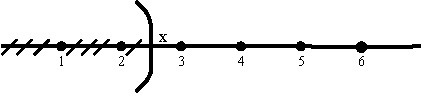
\includegraphics[scale=0.9]{./media/Homework-27-03-20_1.pdf}}
	\end{figure}
	\begin{figure}[H]
		\center{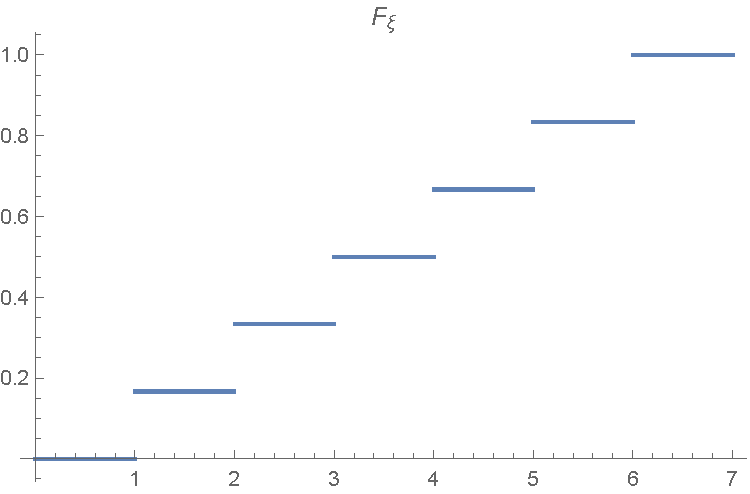
\includegraphics[scale=0.9]{./media/Homework-27-03-20_2.pdf}}
	\end{figure}
\end{exmp}
\begin{exmp}
	Найти функцию распределения решек, выпавших до 1-ого орла при бросании монеты.
	
	$\xi$ - искомая величина (число решек до 1-ого орла), переформулируя,  $\xi$ - число успехов (выпадение решки) до 1-ой неудачи (выпадение орла).
	
	Вероятность выпадения решки: $P(\text{'Р'}) = \frac{1}{2}$.
	
	По формуле испытания Бернулли: $p(\xi = k) = p^k(1-p) = \frac{1}{2} \cdot \frac{1}{2^k} = \frac{1}{2^{k+1}}$.
	\begin{figure}[H]
		\center{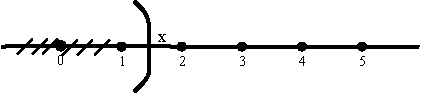
\includegraphics[scale=0.9]{./media/Homework-27-03-20_3.pdf}}
	\end{figure}
	\[ F_{\xi}(x) = \sum_{k < x} P(\xi = k) = \underbrace{\sum_{k=0}^{k<x} \frac{1}{2^{k+1}}}_{\frac{1}{2} + \frac{1}{4} + \frac{1}{8} + \dots} =
	\begin{cases}
	0, x \le 0 \\
	1 - \frac{1}{2^{k+1}}, x \in (k, k+1], k = 0,1,\dots
	\end{cases}
	\]
	где $\sum_{k < x} P(\xi = k)$ - все случаи, когда выпало $<x$.
	\begin{figure}[H]
		\center{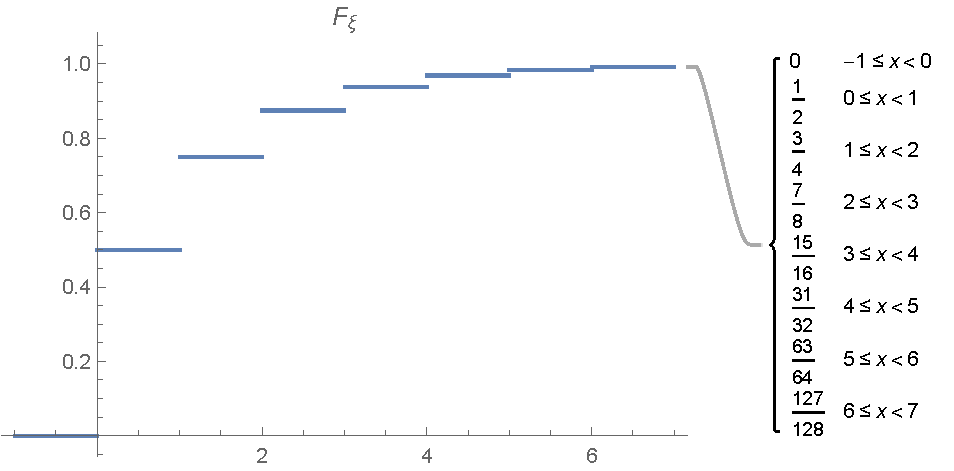
\includegraphics[scale=0.9]{./media/Homework-27-03-20_4.pdf}}
	\end{figure}
\end{exmp}
\begin{exmp}
	Точка бросается наугад в интервале $[0,1], \xi$ - координаты точки.
	\[ F_{\xi}(x) =
	\begin{cases}
	0, x \le 0 \\
	x, x \in (0,1] \\
	1, x > 1 \text{\textcolor{Grey}{ (обязательно будет $\le$ 1)}}
	\end{cases}
	\]
	\[ P(\xi < x) = P(\xi \in[0,1]) \]
	\begin{figure}[H]
		\center{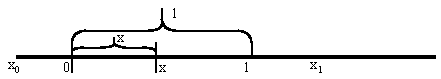
\includegraphics[scale=1]{./media/Homework-27-03-20_5.pdf}}
	\end{figure}
	Вероятность отрезка $[0,x) = \frac{x}{1} = x$.
	\begin{figure}[H]
		\center{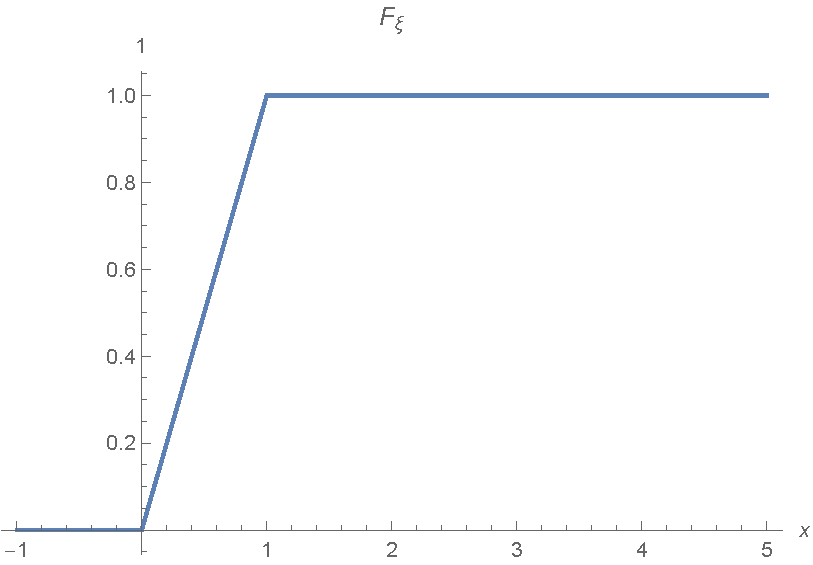
\includegraphics[scale=0.85]{./media/Homework-27-03-20_6.pdf}}
	\end{figure}
	\[ P(\xi < x) = P(\xi \in [0,x)) \]
\end{exmp}

\subsection{Классификация распределений}

\subsubsection{Случайные величины с дискретным законом распределения}

\begin{definition}[Дискретная случайная величина]
	Говорим, что $\xi$ - случайная величина с дискретным законом распределения, если существует $A \subset \mathbb{R}$ такое, что $A$ - не более чем счетное и $P(\xi \in A) = 1$.
	
	Так как $A$ — не более чем счетное, то занумеруем элементы множества $A = \{ a_1, a_2, \dots \}$ и составим следующую таблицу:
	\begin{table}[H]
		\centering
		\begin{tabular}{|c|c|c|c|}
			\hline
			$\xi$ & $a_1$ & $a_2$ & $\dots$ \\ \hline
			$p$   & $p_1$ & $p_2$ & $\dots$ \\ \hline
		\end{tabular}
	\end{table}
	Здесь $p_i = P(\xi = a_i)$. Эту таблицу будем называть законом распределения дискретной случайной величины $\xi$. Отметим, что для чисел $p_i$ выполняются следующие соотношения:
	\begin{enumerate}
		\item $p_i \ge 0$;
		\item $\sum\limits_{i} p_i = 1$.
	\end{enumerate}
	Эти соотношения следуют из свойств вероятностей и равенств:
	\[ 1 = P(\xi \in A) = P \left( \bigcup_i (\xi = a_i) \right) = \sum_{i} P(\xi = a_i) = \sum_{i} p_i \]
\end{definition}

Если случайная величина $\xi$ дискретна, то есть её распределение однозначно задаётся функцией вероятности $P(\xi = a_i) = p_i, p_i \ge 0, \sum\limits_i p_i = 1, i = 1,2,\dots$, то функция распределения $F_{\xi}$ этой случайной величины кусочно-постоянна и может быть записана как:
\[ F_{\xi} (x) = \sum_{i: x_i \le x} p_i. \]
Эта функция непрерывна в любой точке $x \in \mathbb{R}$, такой что $x \ne x_i, \forall i$, и имеет разрыв, равный $p_i$, в $x = x_i$.

\begin{exmp}
	$\xi$ - дискретная, $P(\xi = i)$ задана таблицей распределения. $F_{\xi}(x) - ?$
	\begin{table}[H]
		\centering\makegapedcells
		\begin{tabular}{|c|c|c|c|c|c|c|}
			\hline
			$i$  & 0             & 1             & 2             & 3              & 4              & $\Sigma$ \\ \hline
			вер. & $\frac{1}{8}$ & $\frac{1}{4}$ & $\frac{1}{2}$ & $\frac{1}{16}$ & $\frac{1}{16}$ & 1        \\ \hline
		\end{tabular}
	\end{table}
	
	\noindent \textit{Решение:}
	
	\[ F_{\xi} = \sum_{i=0}^{i<x} P(\xi = i) =
	\begin{cases}
	0, &x \le 0 \\
	\frac{1}{8}, &x \in (0,1] \\
	\frac{1}{8} + \frac{1}{4} = \frac{3}{8}, &x \in (1,2] \\
	\frac{1}{8} + \frac{1}{4} + \frac{1}{2} = \frac{7}{8}, &x \in (2,3] \\
	\frac{1}{8} + \frac{1}{4} + \frac{1}{2} + \frac{1}{16} = \frac{15}{16}, &x \in (3,4] \\
	1, &x > 4
	\end{cases}
	\]
	График распределения данной дискретной случайной величины:
	\begin{figure}[H]
		\center{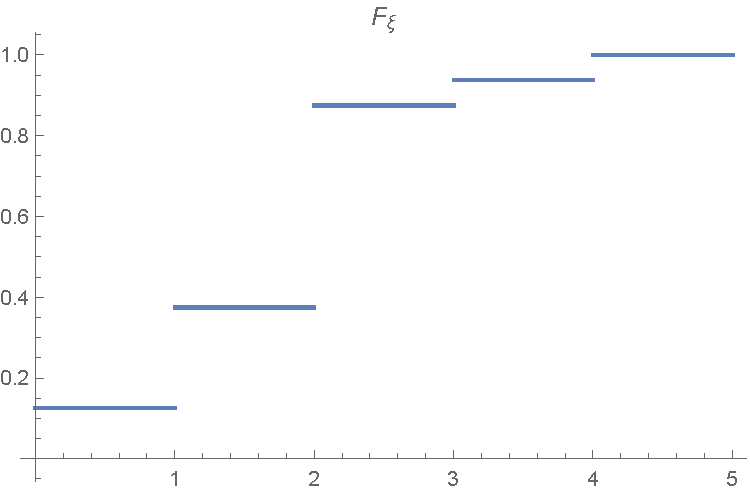
\includegraphics[scale=0.8]{./media/Homework-27-03-20_17.pdf}}
	\end{figure}
\end{exmp}

\begin{exmp}
	Монета подбрасывается 5 раз,
	\begin{enumerate}
		\item[а)] $\xi$ - число орлов, $F_{\xi} - ?$;
		\item[б)] $\xi_1$ - "число орлов"\, - "число решек"\, $F_{\xi_1} - ?$
	\end{enumerate}
	
	\noindent \textit{Решение:}
	
	Формула Бернулли:
	\[ P_n^k = C_n^k p^k q^{n-k} \]
	\noindent где $p$ - вероятность наступления события $A$ (в нашем случае - выпадение орла), которое наступило $k$ раз в $n$ независимых испытаниях, $q=1-p$.
	
	\begin{enumerate}
		\item[а)] Вероятность выпадения как аверса, так и реверса равны $p = \frac{1}{2}$. 
		
		Таким образом, формула для вычислений:
		\[ P(\xi = k) = C_5^k p^k (1 - p)^{n-k} = C_5^k \cdot \left(\frac{1}{2}\right)^k \cdot \left(\frac{1}{2}\right)^{5-k} \]
		\[ P(\xi = 0) = P(\xi = 5) = \underset{=1}{C_5^5} \cdot 
		\begin{cases}
		\left(\frac{1}{2}\right)^1 \cdot \left(\frac{1}{2}\right)^4 = \frac{1}{32} \\
		\left(\frac{1}{2}\right)^5 \cdot \left(\frac{1}{2}\right)^0 = \frac{1}{32}
		\end{cases}
		= \frac{1}{32}
		\]
		\[ P(\xi = 1) = P(\xi = 4) = \frac{5}{32} \]
		\[ P(\xi = 2) = P(\xi = 3) = \frac{10}{32} \]
		
		Следовательно, функция распределения случайной величины выпадения орлов равна:
		\[
		F_{\xi}(x) = \sum_{i=0}^{k<x} P(\xi = k) =
		\begin{cases}
		\frac{1}{32}, &x \in (0,1] \\
		\frac{6}{32} = \frac{3}{16}, &x \in (1,2] \\
		\frac{16}{32} = \frac{1}{2}, &x \in (2,3] \\
		\frac{26}{32} = \frac{13}{16}, &x \in (3,4] \\
		\frac{31}{32}, &x \in (4,5] \\
		1, &x > 5
		\end{cases}
		\]
		График данной функции:
		\begin{figure}[H]
			\center{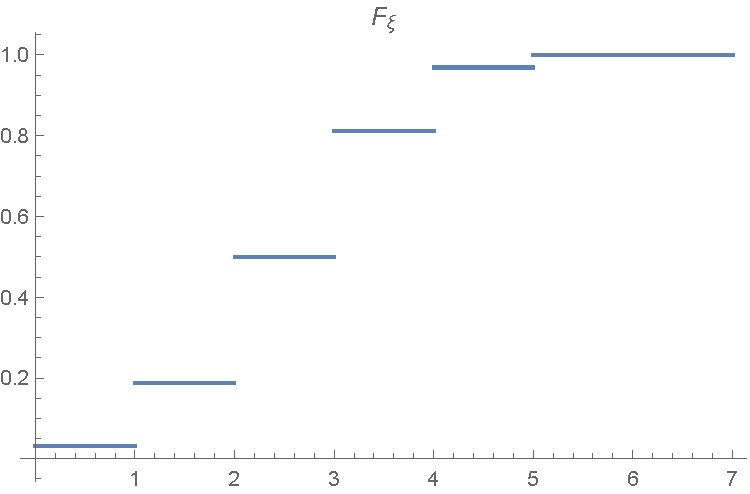
\includegraphics[scale=0.85]{./media/Homework-27-03-20_8.pdf}}
		\end{figure}
		
		\item[б)] Случайная величина $\xi_1$ однозначно определяется $\xi$, т.к. при условии, что не выпадет орёл, обязательно выпадет решка. Т.е. $\xi_1 = \xi - (5 - \xi) = 2\xi - 5$.
		
		Значит, функция распределения обозначенной случайной величины будет равна:
		\[
		F_{\xi_1}(x) = 
		\begin{cases}
		0, &x \le -5 \\
		\frac{1}{32}, &x \in (-5,-3] \\
		\frac{6}{32} = \frac{3}{16}, &x \in (-3,-1] \\
		\frac{16}{32} = \frac{1}{2}, &x \in (-1,1] \\
		\frac{26}{32} = \frac{13}{16}, &x \in (1,3] \\
		\frac{31}{32}, &x \in (3,5] \\
		1, &x > 5
		\end{cases}
		\]
		График данной функции:
		\begin{figure}[H]
			\center{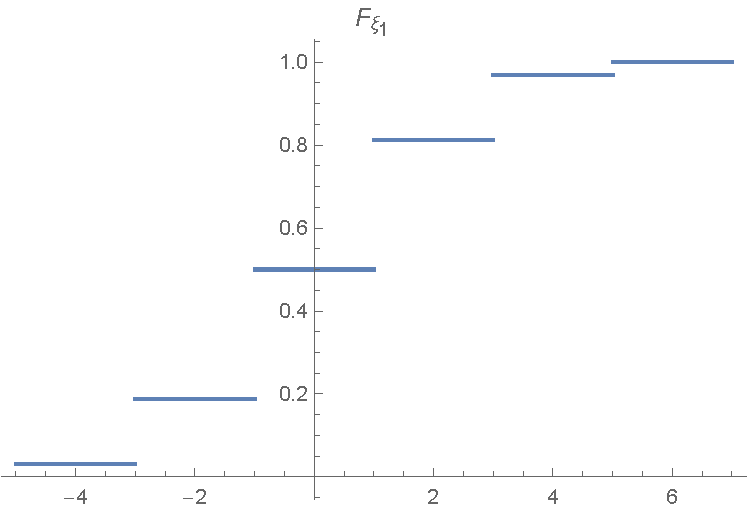
\includegraphics[scale=0.85]{./media/Homework-27-03-20_9.pdf}}
		\end{figure}
		
		Совмещая данные графики, получаем подтверждение утверждения выдвинутого в б) пункте: $\xi_1 = 2\xi - 5$.
		\begin{figure}[H]
			\center{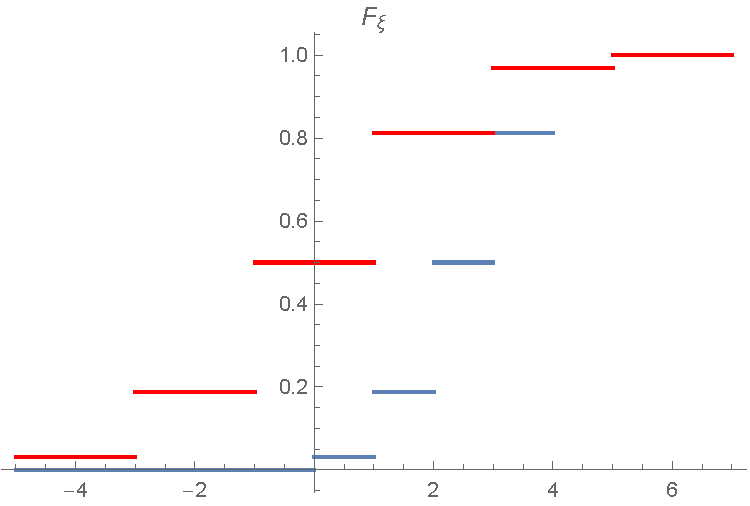
\includegraphics[scale=0.85]{./media/Homework-27-03-20_10.pdf}}
		\end{figure}
	\end{enumerate}
\end{exmp}
\newpage
\subsubsection{Случайные величины с абсолютно непрерывным распределением}

\begin{definition}[Абсолютно непрерывная случайная величина]
	Говорим, что $\xi$ - случайная величина, имеющая абсолютно непрерывное распределение, если существует функция $p_{\xi}$ такая, что для любого $B \in \mathcal{B}$ справедливо равенство
	\[ P(\xi \in B) = \int_B p_{\xi} (x) dx, \]
	где $p_{\xi}$ - некоторая функция, которую будем называть \textit{плотностью распределения случайной величины} (плотность по отношению к мере Лебега) $\xi$.
	
	В частности, если $B = (-\infty; y)$, то
	\[ P(\xi \in B) = F_{\xi} (y) = \int_{-\infty}^{y} p_{\xi} (x) dx \]
	
	Из последнего равенства следует, что $p_{\xi} (x) = F' (x)$ почти всюду.
\end{definition}

\textbf{Свойства функции} $p_{\xi} (x)$

Для плотности случайной величины верны следующие соотношения, справедливость которых непосредственно следует из определения,
\begin{enumerate}
	\item $p_{\xi} (x) \ge 0$ почти всюду;
	\item $\int\limits_{-\infty}^{\infty} p_{\xi} (x) dx = 1$.
\end{enumerate}

\subsubsection{Дискретные и абсолютно непрерывные случайные величины}

\begin{figure}[h]
	\center{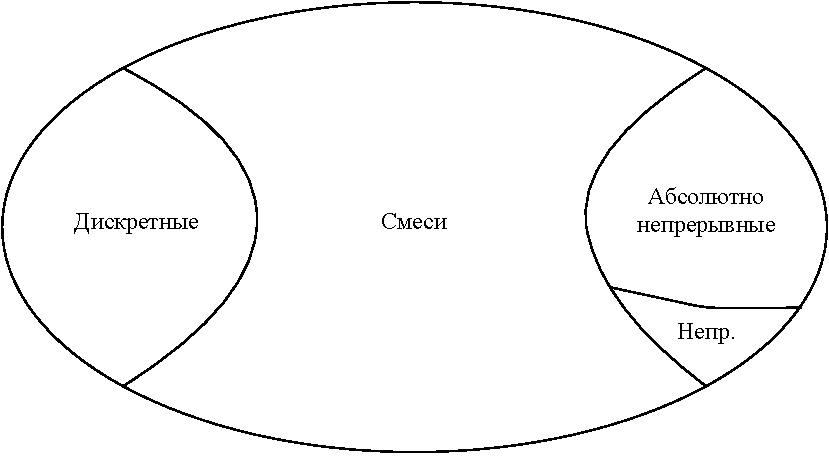
\includegraphics[scale=0.8]{./media/1.14.pdf}}
\end{figure}
Для любого распределения случайной величины $\exists$ представление:
\[ \mathcal{P} = \alpha \mathcal{P}_{\xi}^c + (1 - \alpha) \mathcal{P}_{\xi}^{d} \]
$\mathcal{P}_{\xi}^{\alpha}$ - дискретное, $\mathcal{P}_{\xi}^{c}$ - непрерывное, $\alpha \in [0, 1]$.

\begin{definition}[Носитель распределения случайной величины]
	Носителем распределения (или множеством значений) случайной величины $\xi$ называется любое борелевское множество $N_{\xi} \in \mathbb{R}$ такое, что $P(\xi \notin N_{\xi}) = 0$. В частности, образ множества $\Omega$ при отображении $\xi$ является носителем распределения $\xi$. Будем говорить, что \textit{носитель распределения} $\xi$ \textit{содержится в множестве} $A$, если существует носитель распределения $\xi$, содержащийся в данном множестве. Отметим, что носитель распределения определяется однозначно с точностью до множеств меры 0 ($P(N_{\xi}^{(1)} \triangle N_{\xi}^{(2)}) = 0$). Распределение случайной величины полностью характеризуется значениями на измеримых подмножествах носителя.
\end{definition}

\subsubsection{Преобразование случайных величин}

\noindent\textbf{Постановка проблемы.}
Пусть $(\Omega, \mathcal{F}, P)$ - вероятностный эксперимент, $\xi$ - случайная величина. Если функция $f: \mathbb{R} \to \mathbb{R}$ такова, что $\eta = f(\xi)$ - случайная величина, то нужно уметь находить распределение $\eta$ по распределению $\xi$.

\begin{remark}
	Эта проблема возникает, например, при моделировании случайных величин с заданным распределением. Датчик случайных чисел может генерировать лишь значения случайных величин с равномерным распределением. А если нам необходимы значения показательно распределённой случайной величины, нужно знать, какое преобразование применить, чтобы из равномерного распределения получить показательное.
\end{remark}

\begin{figure}[H]
	\center{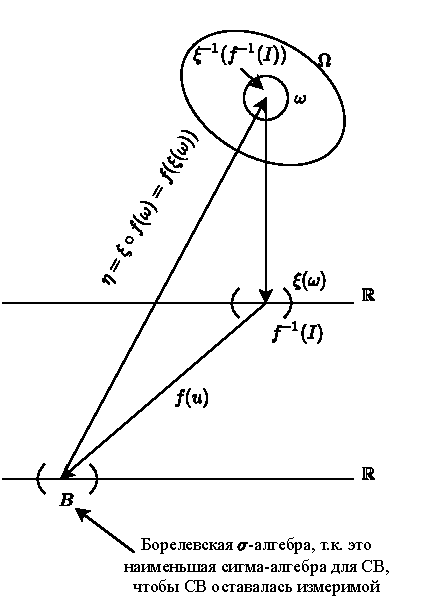
\includegraphics[scale=1]{./media/random_conversion.pdf}}
\end{figure}

Вопрос об измеримости $\eta$ решает следующая теорема:

\begin{theorem}
	Пусть $\xi$ - случайная величина.
	\noindent $f: \mathbb{R} \to \mathbb{R}$ - борелевская (измеримая по Борелю) функция, т.е. такая, что для всякого борелевского множества $B$ его прообраз $f^{-1} (B)$ есть снова борелевское множество, тогда $\eta = f (\xi)$ - \textit{случайная величина}.
	\begin{proof}
		Проверим, что прообраз любого борелевского множества при отображении $f(\xi): \Omega \to \mathbb{R}$ является \textit{событием}. Возьмём произвольное $B \in \Borel (\mathbb{R})$ и положим $B_1 = f^{-1} (B)$. Множество $B_1$ борелевское, так как функция $f$ измерима по Борелю. Найдём:
		\[ ( f(\xi) )^{-1} (B) = \eta^{-1} (B) = \{ \omega | f (\xi(\omega)) \in B \} = \{ \omega | \xi (\omega) \in f^{-1} (B) = B_1 \} = \xi^{-1} (B_1) \in \Event, \]
		поскольку $B_1 \in \Borel (\mathbb{R})$ и $\xi$ - случайная величина.
	\end{proof}
\end{theorem}

\begin{remark}
	Борелевскими являются все привычные нам функции. Функцией, неизмеримой по Борелю, будет, например, индикаторная функция неизмеримого множества Витали, т.е. функция, принимающая значение 1 в точках этого множества и значение 0 во всех прочих точках числовой прямой. Вообще говоря, неизмеримые функции суть объекты экзотические, в обычной жизни не встречающиеся.
\end{remark}

Известны: распределение $\xi: \mathcal{P}_{\xi}$, функция $f$.
\[ \mathcal{P}_{\eta} (B) = P(\omega : \eta(\omega) \in B) = P(\omega : f(\xi(\omega)) \in B) = P(\omega : \xi (\omega) \in f^{-1} (B)) = \mathcal{P}_{\xi} (f^{-1} (B)) - \text{ \textbf{распределение} } \eta \]
\[ f^{-1} (B) = \{ y \in \mathbb{R} : f(y) \in B \} - \text{ \textbf{прообраз} } B \]

\noindent\textbf{В терминах функции распределения.}
\[ F_{\eta} (y) = P(\eta < y) = P(f(\xi) < y) = P(\xi \in f^{-1} ((- \infty, y))) = \mathcal{P}_{\eta} (f^{-1}(- \infty, y)) \]

\textit{Частный случай:}

\noindent $f$ монотонна (строго монотонна) в точке $x$.
\[ 	f(u) = f(x) \Rightarrow u = x \]
\begin{enumerate}
	\item $f(t) \le f(u), t < u$ - возрастает;
	\item $f(t) \ge f(u), t < u$ - убывает.
\end{enumerate}
\[ f(\xi) < y \eq 1) \xi < f^{-1} (\{y\}); 2) \xi > f^{-1} (\{y\}) \]
$f$ - строго монотонна $\forall x \in \supp (\xi)$
\[
F_{\eta} (y) =
\left[
	\begin{array}{c}
		F_{\xi} (f^{-1}(y)), \text{ стр. возр.} \\
		1 - F_{\xi} (f^{-1} (y)_{+}), \text{ стр. убыв.} \\
	\end{array}
\right.
\]

\begin{exmp}[Преобразование Гауссова распределения]
	\[ \mathcal{P}_{\xi} (x) = \frac{1}{\sqrt{2 \pi}} e^{- \frac{x^2}{2}}, x \in \mathbb{R} \]
	Пусть $\eta = \xi^2$
	\[ S_{\eta} : P(S_{\eta} = 1) - \text{ носитель распределения}, S_{\eta} = [0, \infty] \]
	\[ F_{\eta} (y) = P(\xi^2 < y) = P(|\xi| < \sqrt{y}) = p(- \sqrt{y} < |\xi| < \sqrt{y}) = \int_{-\sqrt{y}}^{\sqrt{y}} \frac{1}{\sqrt{2 \pi}} e^{- \frac{t^2}{2}} dt = \] 
	\[ = 2 \int_{0}^{\sqrt{y}} \frac{1}{\sqrt{2 \pi}} e^{-\frac{t^2}{2}} dt = 2 \Phi (\sqrt{y}), y > 0 \]
	\[
	F_{\eta}' (y) =
	\begin{cases}
		0, & y < 0 \\
		\frac{1}{\sqrt{y}} \Phi' (\sqrt{y}), y > 0
	\end{cases}
	~~~~~~~~~
	P_{\eta} =
	\begin{cases}
		0, & y \le 0 \\
		\frac{1}{\sqrt{2 \pi y}} e^{- \frac{y}{2}}, y > 0
	\end{cases}
	- \chi^2 \text{ с одной степенью свободы}
	\]
\end{exmp}

\noindent \textbf{Преобразование дискретного распределения}

Пусть $supp(\xi)=E$ - не более, чем счетно

\noindent $\eta=f(\xi)$ - дискретная случайная величина ($f(E)$ - не более чем счетно)
\[P(\eta = b_j) = P(\xi \in f^{-1}(\{b_j\}) = \sum\limits_{i:f(a_i)=b_j} P(\xi = a_i) \]

\begin{exmp}
	Имеется следующее распределение:
	\begin{table}[H]
		\centering
		\begin{tabular}{|c|c|c|c|}
			\hline
			$\xi$ & $-1$  & $0$   & $1$   \\ \hline
			$P$   & $1/3$ & $1/3$ & $1/3$ \\ \hline
		\end{tabular}
	\end{table}
	\[ \eta = \xi^2; ~~~~~~~~~ S_{\eta} = \{0,1\} \]
	\[ P(\eta = 0) = P(\xi = 0) = \frac{1}{3} \]
	\[ P(\eta = 1) = P(\xi = 1) + P(\xi = -1) = \frac{2}{3} \]
\end{exmp}

\begin{exmp}
	\[ p_i = \frac{1}{2^{i + 1}}; i = 0,1,\dots \]
	\[ \eta = \cos \left( \frac{\pi \xi}{2} \right) \]
	
	\noindent $S_{\xi} = \{ 0,1,\dots \}$ - носитель $\xi$
	
	\noindent $S_{\eta} = \{ -1,0,1 \}$ - носитель $\eta$
	
	\[ P(\eta = 0) = P \left( \cos \left( \frac{\pi \xi}{2} \right) = 0 \right) = \sum_{k=0}^{\infty} P \left( \frac{\pi \xi}{2} = \frac{\pi}{2} + 2 \pi k \right) = \sum_{k=0}^{\infty} P (\xi + 1 = 2k) = \sum_{k=0}^{\infty} \frac{1}{2^{2k+2}} = \frac{1}{3} \]
	\[ P(\eta = 1) P \left( \cos \left( \frac{\pi \xi}{2} \right) = 1 \right) = \sum_{k=0}^{\infty} P \left( \frac{\pi \xi}{2} = 2 \pi k \right) = \sum_{k=0}^{\infty} (\xi = 4k) = \sum_{k=0}^{\infty} \frac{1}{2^{1 + 4k}} = \frac{8}{15} \]
	\[ P(\eta = -1) = \sum_{k=0}^{\infty} P \left( \frac{\pi \xi}{2} = \pi + 2 \pi k \right) = \sum_{k=0}^{\infty} P (\xi = 2 + 4k) = \frac{1}{2^{3 + 4k}} = \frac{2}{15} \]
	\begin{table}[H]
		\centering
		\begin{tabular}{|c|c|c|c|}
			\hline
			$-1$   & $0$   & $1$    & $\Sigma$ \\ \hline
			$2/15$ & $1/3$ & $8/15$ & $1$      \\ \hline
		\end{tabular}
	\end{table}
\end{exmp}

\noindent \textbf{Преобразование абсолютно непрерывных распределений}

Пусть $\xi$ - абсолютно непрерывное распределение, $p_\xi$ - плотность распределения, $f$ - функция, $\eta = f(\xi), \exists f^{-1}$
\[F_\eta(x)=P(\eta<y) = P(f(\xi)<y)\]
\begin{enumerate}
	\item $f$ - строго возрастает и дифференцируема
	\[F_\eta(y)=P(\xi < f^{-1}(y))\]
	\[p_\eta(y)=\dfrac{1}{f'(f^{-1}(y))}p_\xi(f^{-1}(y))\]
	\item $f$ - строго убывает и дифференцируема
	\[F_\eta(y)=P(\xi > f^{-1}(y))\]
	\[p_\eta(y)=-\dfrac{1}{f'(f^{-1}(y))}p_\xi(f^{-1}(y))\]
	\item $f$ - строго монотонна и дифференцируема
	\[p_\eta(y)=\dfrac{1}{|f'(f^{-1}(y))|}p_\xi(f^{-1}(y))\]
\end{enumerate}

\begin{exmp}[Преобразование показательного распределения]
	\[
	p_{\xi} (x) =
	\begin{cases}
		ae^{-ax}, & x \ge 0 \\
		0, & x < 0
	\end{cases};
	a \in \mathbb{R}_{\ge 0}
	\]
	\[ f(t) = e^t ~~~~~~~~~ f^{-1} (y) = \ln y \]
	\[
	p_{\eta} (y) =
	\begin{cases}
		0, & y \le 1 \\
		\frac{1}{e^{\ln y}} e^{- \ln y}, & y > 1
	\end{cases}
	=
	\begin{cases}
		0, & y \le 1 \\
		\frac{1}{y^2}, & y > 1
	\end{cases}
	\]
	\[ S_{\eta} = [1, \infty] \]
	\[ \int_{1}^{\infty} \frac{1}{y^2} dy = - \frac{1}{y} \bigg|_{1}^{\infty} = 1 \]
\end{exmp}

\noindent \textbf{Линейное преобразование}

$\xi \curvearrowright \beta$ - плотность распределения $\xi$.
\[ \eta = a \xi + b; a \ne 0 (\text{при } a = 0: P(\eta = n) = 1) \]
\[
	F_{\eta} (x) = P(\eta < x) = P(a \xi + b < x) = P(a \xi < x - b) =
	\begin{cases}
		F_{\xi} \left( \frac{x - b}{a} \right), & a > 0 \\
		1 - F_{\xi} \left( \frac{x - b}{a} \right), & a < 0
	\end{cases}
\]
\[ p_{\eta} (x) = \frac{1}{|a|} p_{\xi} \left( \frac{x - b}{a} \right) \]

\noindent \textbf{Преобразование Смирнова}

Пусть $\xi$ - непрерывная, $F_{\xi}$ - функция распределения $\xi$ Задача: имея выборку из стандартного непрерывного равномерного распределения, получить выборку распределения из $F_{\xi}$.
\[ \eta = F_{\xi} (\xi) \sim U(0,1), \text{ т.е.} \]
\[
\eta - \text{ абсолютно непрерывная и } p_{\eta}(x) =
\begin{cases}
	1, & x \in [0, 1] \\
	0, & x \notin [0, 1]
\end{cases}
\]
Пусть $F_{\xi}$ - строго возрастает ($\exists F_{\xi}^{-1}$)
\[ P(\eta < x) = P(F_{\xi} (\xi) < x) = P(\xi < F_{\xi}^{-1} (x)) = F_{\xi} (F_{\xi}^{-1} (x)) = x, x \in [0, 1] \]
\[
F_{\eta} (x) =
\begin{cases}
	0, & x \le 0 \\
	x, & x \in [0, 1] \\
	1, & x > 1
\end{cases};
~~~~~~
p_{\eta} (x) =
\begin{cases}
	1, & x \in [0, 1] \\
	0, & x \notin [0, 1]
\end{cases}
\]
Получается, что случайная величина $\eta$ имеет равномерное распределение на $[0, 1]$, и у случайной величины $F_{\xi}^{-1} (\eta)$ такое же распределение, как и у $\xi$.

Так что если есть выборка $U_1, \dots, U_n \sim U(0, 1)$, то интересующая нас выборка - $X_1, \dots, X_n$ - имеет члены вида $X_i = F_{\xi}^{-1} (U_i), i = 1, \dots, n$.

\subsubsection{Некоторые законы распределения}

\noindent \textbf{Дискретные законы распределения.}
\begin{enumerate}
	\item Биномиальное распределение. Случайная величин $\xi$ может принимать значения $m = 0,1,2,\dots,n$. Соответствующие вероятности
	\[ p_m = P(\xi = m) = C_n^m p^m (1-p)^{n-m}, \text{ где } 0 < p < 1 \]
	\item Гипергеометрическое распределение. Случайная величина $\xi$ может принимать значения $m = 0,1,2,\dots, \min (n, M)$. Соответствующие вероятности
	\[ p_m = P(\xi = m) = \frac{C_M^mC_{N-M}^{n-m}}{C_N^n}, \]
	где $n, M$ и $N$ - натуральные числа, причем $n, M \le N$.
	\item Распределение Пуассона. Случайная величина $\xi$ может принимать значения $m = 0,1,2,\dots$. Соответствующие вероятности
	\[ p_m = P(\xi = m) = \lambda^m \frac{e^{- \lambda}}{m!}, \text{ где } \lambda > 0. \]
	\item Геометрическое распределение. Случайная величина $\xi$ может принимать значения $m = 1,2,\dots$. Соответствующие вероятности
	\[ p_m = P(\xi = m) = (1 - p)^{m-1}p, \text{ где } 0 < p < 1. \]
	\item Распределение Бернулли. Случайная величина $\xi$ с таким распределением равна числу успехов в одном испытании схемы Бернулли с вероятностью $p$ успеха : ни одного успеха или один успех. Функция распределения $\xi$ имеет вид:
	\[
	F_{\xi} (x) = P (\xi < x) =
	\begin{cases}
		0, & x \le 0 \\
		1 - p, & 0 < x \le 1 \\
		1, & x > 1
	\end{cases}
	\]
	Мат. ожидание: $E\xi = p$. Дисперсия: $D\xi = p(1-p) = pq$, так как $E\xi^2 - (E\xi)^2 = p - p^2 = p \cdot (1-p) = pq$.
\end{enumerate}

\noindent \textbf{Непрерывные законы распределения.}
\begin{enumerate}
	\item Равномерное распределение на отрезке $\xi \in U[a, b]$. Плотность распределения задается функцией:
	\[
	p(x) =
	\begin{cases}
		\frac{1}{b-a}, &x \in [a, b] \\
		0, &x \notin [a, b]
	\end{cases}
	\]
	Это непрерывное распределение, у которого плотность почти всюду постоянна.
	Мат. ожидание, моменты и дисперсия:
	\[E(X)=\dfrac{a+b}{2}\]
	\[E(X^2)=\dfrac{a^2+ab+b^2}{3}\]
	\[D(X)=\dfrac{(b-a)^2}{12}\]
	Стандартное равномерное распределение - это $U[0,1]$
	\item Нормальное (гауссово) распределение - $\xi \in N(a, \sigma^2)$ - непрерывное распределение.

	Здесь $a$ - математическое ожидание, $ \sigma^2$ - дисперсия.
	\[ p(x) = \frac{1}{\sqrt{2 \pi} \sigma} \exp \left\{ - \frac{(x-a)^2}{2 \sigma^2} \right\} \]
	Стандартное нормальное распределение - это $N(0,1)$.
	Его плотность вероятности:
	\[ p(x) = \dfrac{1}{\sqrt{2\pi}}\exp(-\frac{1}{2}x^2)\]
	
	\item Распределение Пуассона $\xi \in Pois(\lambda)$ - распределение дискретного типа случайной величины (представляющей собой число событий, произошедших за фиксированное время)
	
	Здесь $\lambda$ - математическое ожидание и дисперсия (они равны).
	\[p(x)=\frac{\lambda^x}{x!}e^{-\lambda}, \lambda>0\]
	\item Показательное распределение с параметром $\lambda > 0$:
	\[
	p(x) =
	\begin{cases}
		\lambda e^{- \lambda x}, &x \ge 0 \\
		0, &x  < 0
	\end{cases}
	\]
	\item Распределение Максвелла:
	\[
	p(x) =
	\begin{cases}
		\sqrt{\frac{2}{\pi \sigma^3}} x^2 \exp \left\{ - \frac{x^2}{2 \sigma^2} \right\}, &x \ge 0 \\
		0, &x < 0
	\end{cases}
	\]
	\item Распределение Стьюдента с $n$ степенями свободы:
	\[ p(x) = \frac{\Gamma \left( \frac{n+1}{n} \right)}{\sqrt{\pi n} \Gamma \left(\frac{n}{2}\right)} \left( 1 +  \frac{x^2}{n} \right)^{-\frac{n+1}{2}} \]
	\item Говорят, что $\xi$ имеет \textit{гамма-распределение} с параметрами $\alpha > 0, \gamma > 0$, и пишут: $\xi \in \Gamma_{\alpha, \lambda}$, если $\xi$ имеет следующую плотность распределения:
	\[
	p_{\xi} (x) =
	\begin{cases}
		0, & \text{ если } x \le 0 \\
		c \cdot x^{\lambda -1} e^{- \alpha x}, & \text{ если} x > 0
	\end{cases}
	\]
	где постоянная $c$ вычисляется из свойства плотности так:
	\[ 1 = \int\limits_{- \infty}^{\infty} p_{\xi} (x) dx = c \int\limits_{0}^{\infty} x^{\lambda - 1} e^{- \alpha x} dx = \frac{c}{\alpha^{\lambda}} \int\limits_{0}^{\infty} (\alpha x)^{\lambda - 1} e^{- \alpha x} d (\alpha x) = \frac{c}{\alpha^{\lambda}} \Gamma (\lambda), \]
	откуда $c = \frac{\alpha^{\lambda}}{\Gamma (\lambda)}$. Здесь через $\Gamma (\lambda)$ обозначена гамма-функция Эйлера:
	\[ \Gamma (\lambda) = \int\limits_{0}^{\infty} x^{\lambda - 1} e^{-x} dx = (\lambda - 1) \Gamma(\lambda - 1) \]
	\[ \Gamma (k) = (k - 1)! \text{ при целых положительных } k \]
	\[ \Gamma (1) = 1 \]
	Показательное распределение — частный случай гамма-распределения: $E_{\alpha} = \Gamma_{\alpha, 1}$.
	\item Пусть распределение случайной величины $\xi$ задаётся плотностью вероятности $p_{\xi} (x)$, имеющий вид:
	\[ p_{\xi} (x) = \frac{1}{B(\alpha, \beta)} x^{\alpha - 1} (1 - x)^{\beta - 1}, \]
	где
	\begin{itemize}
		\item $\alpha, \beta$ - произвольные фиксированные параметры, и
		\item $B(\alpha, \beta) = \int\limits_{0}^{1} x^{\alpha - 1} (1 - x)^{\beta - 1} dx$ - бета-функция.
	\end{itemize}
	Тогда случайная величина $\xi$ имеет бета-распределение. Пишут: $\xi \sim B(\alpha, \beta)$.
	\item Распределение хи-квадрат с $n$ степенями свободы:
	\[
	p(x) =
	\begin{cases}
		\frac{1}{2^{\frac{n}{2}} \Gamma \left(\frac{n}{2}\right)} x^{\frac{n}{2} - 1} e^{- \frac{x}{2}}, &x \ge 0 \\
		0, &x < 0
	\end{cases}
	\]
\end{enumerate}
Здесь $\Gamma(s)$ - гамма-функция.

Методами математического анализа можно показать, что функции $p(x)$, указанные выше, удовлетворяют условию
нормировки:
\[ \int_{-\infty}^{\infty} p(x) = 1 \]

\subsection{Независимость случайных величин}

\begin{definition}[Независимые случайные величины]
	Пусть на некотором вероятностном пространстве $(\Omega, \mathcal{F}, P)$ определены $\xi_1, \dots, \xi_n$ - случайные величины, $\vec{\xi} = (\xi_1, \dots, \xi_n)$ - соответствующий случайный вектор. $\mathcal{P}_{\xi_1, \dots, \xi_n}$ - распределение ($F_{\xi_1, \dots, \xi_n}$ - ф-я распределения), $p_{\xi_1, \dots, \xi_n}$ - плотность распределения. $B_1, \dots, B_n$ - борелевские подмножества множества вещественных чисел, $B_1, \dots, B_n \in \mathcal{B}$ - множество борелевских подмножеств множества вещественных чисел (борелевская $\sigma$-алгебра).
	
	\textit{В терминах борелевских подмножеств:}
	
	\[ P(\xi_1 \in B_1, \dots, \xi_n \in B_n) = \prod_{i=1}^{n} P(\xi_i \in B_i) \]
	
	\textit{В терминах распределения случайного вектора:}
	
	\[ \mathcal{P}_{\vec{\xi}} (B_1 \times \dots \times B_n) = \mathcal{P}_{\vec{\xi}} (B_1 \times \mathbb{R} \times \dots \times \mathbb{R}) \cdot \mathcal{P}_{\vec{\xi}} (\mathbb{R} \times B_2 \times \dots \times \mathbb{R}) \cdot ... \cdot \mathcal{P}_{\vec{\xi}} (\mathbb{R} \times ... \times \mathbb{R} \times B_n) \]
	
	\textit{В терминах функций распределения:}
	
	Говорим, что $\xi_1, \dots, \xi_n$ - независимые случайные величины, если для любых $x_1, x_2, \dots, x_n \in \mathbb{R}$ при условии совпадения всех функций распределений справедливо равенство:
	
	\[ F_{\vec{\xi}} (x_1 \dots x_n) = \underset{F_{\vec{\xi}}(x_1, \infty, \dots, \infty)}{F_{\xi_1}(x_1)} \cdot ... \cdot \underset{F_{\vec{\xi}}(\infty, \dots, \infty, x_n)}{F_{\xi_n}(x_n)} = \prod_{i=1}^{n} F_{\xi_i} (x_i) \]
	Это означает, что
	\[ P(\xi_1 < x_1, \dots, \xi_n < x_n) = \prod_{i=1}^{n} P(\xi_i < x_i) \]
	Заметим, что здесь речь идет о независимости в совокупности.
	
	\textit{В терминах плотностей:}
	
	Для абсолютно непрерывных величин независимость можно задать в терминах плотностей: для любых $x_1, x_2, \dots, x_n \in \mathbb{R}$:
	\[ p_{\vec{\xi}} (x_1 \dots x_n) = p_{\xi_1} (x_1) \dots p_{\xi_n} (x_n) \]
	\[ p_{\xi_i} (x_i) = \int_{\mathbb{R}^{n-1}} p_{\vec{\xi}} (\vec{x}) dx_1 \dots dx_{i-1} dx_{i+1} \dots dx_n \]
\end{definition}

\subsection{Числовые характеристики случайных величин}

Пусть $(\Omega, \mathcal{F}, P)$ - вероятностный эксперимент, в котором определена случайная величина $\xi$, и $\mathcal{P}_{\xi}$ - её распределение.

\subsubsection{Математическое ожидание случайной величины}

\begin{definition}[Мат. ожидание]
	Математическим ожиданием случайной величины $\xi$ называют \textbf{число} $E\xi$, определяемое равенством
	\[ E\xi = \int_{\omega \in \Omega} \xi (\omega) d P(\omega) = \int_{-\infty}^{\infty} x dF_{\xi} (x) = 
	\left[
		\begin{array}{c}
			\sum\limits_{i: p_i > 0} a_i p_i, p_i = P(\xi = a_i), \sum_{i} p_i = 1 \text{ (дискретное)} \\
			\int\limits_{\mathbb{R}} x p_{\xi} (x) dx, p_{\xi} - \text{ плотность распределения } \xi (\exists \text{ если } \int \text{ сход.})
		\end{array}
	\right.
	\]
	где $F_{\xi}$ - функция распределения величины $\xi$.
	Если оно (это число) существует. Если интеграл расходится, то говорят, что у случайной величины отсутствует математическое ожидание.
\end{definition}

\begin{remark}
	Математическое ожидание часто еще называют средним случайной величины. Предположим, что у случайной величины $\xi$ ровно $n$ значений, и все $p_i = \frac{1}{n}$, тогда $\xi = \frac{1}{n} \sum\limits_{i} a_i$ - среднее арифметическое значений случайной величины.
\end{remark}

\begin{center}
	\textbf{Свойства математического ожидания}
\end{center}
\begin{enumerate}
	\item Если $P(\xi = c) = 1$, то $E\xi = c$.
	\item Линейность математического ожидания. Пусть $\xi, \eta$ - случайные величины. Тогда для любых $\alpha, \beta \in \mathbb{R}$ справедливо равенство: $E(\alpha \xi + \beta \eta) = \alpha E \xi + \beta E \eta$. В данном случае предполагаем, что математические ожидания, о которых идет речь, существуют.
	\item Если $P(\xi \ge 0) = 1$, то $E\xi \ge 0$.
	\item Если $P(\xi \ge \eta) = 1$, то $E\xi \ge E\eta$.
	\item Справедливо неравенство $|E\xi| \le E |\xi|$.
\end{enumerate}

\subsubsection{Моментные характеристики}

\begin{definition}[Момент]
	Моментом порядка $k$ случайной величины $\xi$ называется число $E\xi^k$. Значение $E(\xi - E\xi)^k$ называется центральным моментом порядка $k$, так что дисперсия есть центральный второй момент $\xi$.
	
	Если дан случайный вектор $(\xi_1, \dots, \xi_n)$, то величина $E\xi_1^{k_1} \dots E\xi_n^{k_n}$ называется \textit{смешанным моментом} порядка $k_1 + \dots + k_n$. Аналогично $E(\xi_1 - E\xi_1)^{k_1} \dots E(\xi_n - E\xi_n)^{k_n}$ называется центральным смешанным моментом того же порядка.
\end{definition}

Для независимых величин смешанные моменты равны, очевидно, произведению соответствующих обычных моментов.

\subsubsection{Дисперсия (степень рассеяния)}\label{dispersion}

\begin{definition}[Дисперсия]
	Дисперсией случайной величины $\xi$ называется центральный момент второго порядка $E(\xi - E\xi)^2$, если этот момент существует.
	
	Стандартное обозначение для дисперсии - $D\xi$.
	
	Из определения математического ожидания следует, что
	\[ D\xi = \int_{\Omega} ( \xi (\omega) - E\xi )^2 d P(\omega) \]
	
	Таким образом, дисперсия — это среднее значение квадрата отклонения случайной величины от её математического ожидания.
\end{definition}

\begin{center}
	\textbf{Свойства дисперсии}
\end{center}
\begin{enumerate}
	\item $D\xi \ge 0$ и $D\xi = 0$ тогда и только тогда, когда $P(\xi = c) = 1$ для некоторого $c \in \mathbb{R}$ (т.е. случайная величина $\xi$ имеет вырожденное распределение).
	\item Если $\alpha, \beta \in \mathbb{R}$, то $D(\alpha \xi + \beta) = \alpha^2 D\xi$
	\item $D\xi = E\xi^2 - (E\xi)^2$
	\item $D(\xi + \eta) = D\xi + D\eta + 2E (\xi - E\xi) (\eta - E\eta)$
	\item Если $\xi$ и $\eta$ - независимые случайные величины и существуют их дисперсии, то $D(\xi + \eta) = D\xi + D \eta$. Верно и для произвольного числа попарно независимых случайных величин. В обратную сторону неверно.
\end{enumerate}
\begin{remark}
	Дисперсия разности: $D(\xi - \eta) = D\xi + D(-\eta) = D\xi + D\eta$, т.е. дисперсия разности – это НЕ разность дисперсий.
\end{remark}

\begin{center}
	\textbf{Математическое ожидание и дисперсия — это характеристики именно распределения случайной величины!}
\end{center}

\subsubsection{Примеры вычисления мат. ожидания и дисперсии}

\begin{exmp}[Мат. ожидание для дискретной величины]
	\noindent\textit{\textbf{Условие:}}
	
	Функция распределения случайной величины $\xi$:
	\[
	F_{\xi} (x) =
	\begin{cases}
	0, &x \le 0 \\
	\frac{1}{3}, &x \in (0, 1] \\
	\frac{1}{2}, &x \in (1, 3] \\
	1, &x >3
	\end{cases}
	\]
	Найти $E\xi - ?, D\xi - ?$
	
	\noindent\textit{\textbf{Решение:}}
	
	Таблица дискретного распределения:
	\begin{table}[H]
		\centering\makegapedcells
		\begin{tabular}{|c|c|c|c|}
			\hline
			$k$        & 0             & 1                                     & 3             \\ \hline
			$P(\xi=k)$ & $\frac{1}{3}$ & $\frac{1}{2}-\frac{1}{3}=\frac{1}{6}$ & $\frac{1}{2}$ \\ \hline
		\end{tabular}
	\end{table}
	Т.к. величина дискретная $\Rightarrow$
	\[
	E\xi = \sum_{k} k \cdot P(\xi = k) = 0 \cdot \frac{1}{3} + 1 \cdot \frac{1}{6} + 3 \cdot \frac{1}{2} = \frac{5}{3}
	\]
	\[
	E\xi^2 = 0^2 \cdot \frac{1}{3} + 1^2 \cdot \frac{1}{6} + 3^2 \cdot \frac{1}{2} = \frac{14}{3}
	\]
	\[
	D\xi = E(\xi - E\xi)^2 = E\xi^2 - (E\xi)^2 = \frac{14}{3} + \left( \frac{5}{3} \right)^2 = \frac{17}{9}
	\]
\end{exmp}

\begin{exmp}[Мат. ожидание для абс. непрерывной величины]
	\noindent\textit{\textbf{Условие:}}
	
	Плотность распределения случайной величины $\xi$:
	\[
	p_{\xi} (x) = \frac{1}{2} e^{-|x|}, x \in \mathbb{R}
	\]
	Найти $E\xi - ?, D\xi - ?$
	
	\noindent\textit{\textbf{Решение:}}
	
	Избавимся от модуля:
	\[
	p_{\xi}(x) =
	\begin{cases}
		\frac{1}{2} e^{-x}, &x \ge 0 \\
		\frac{1}{2} e^x, &x < 0
	\end{cases}
	\]
	
	\[
	E\xi = \int_{-\infty}^{\infty} x p_{\xi} (x) dx = \int_{-\infty}^{0} \frac{1}{2} x e^x dx + \int_{0}^{\infty} \frac{1}{2} x e^{-x} dx = \dots = 0
	\]
	\[
	E\xi^2 = \int_{-\infty}^{\infty} x^2 \cdot p_{\xi}(x) dx = \int_{-\infty}^{0} \frac{1}{2} x^2 e^x dx + \int_{0}^{\infty} \frac{1}{2} x^2 e^{-x} dx = \dots = 2
	\]
	\[
	D\xi = E\xi^2 - (E\xi)^2 = 2
	\]
\end{exmp}

\begin{exmp}[Распределение с несуществующим мат. ожиданием]
	\noindent\textit{\textbf{Условие:}}
	
	Функция распределения случайной величины $\xi$:
	\[
	F_{\xi} (x) =
	\begin{cases}
		0, &x \le 1 \\
		1 - \frac{1}{x^2}, &x > 1
	\end{cases}
	\]
	Найти $E\xi - ?, D\xi - ?$
	
	\noindent\textit{\textbf{Решение:}}
	
	Плотность распределения:
	\[
	p_{\xi} =
	\begin{cases}
		0, & x < 1 \\
		\frac{2}{x^3}, &x \ge 1
	\end{cases}
	\]
	
	\[
	E\xi \int_{-\infty}^{\infty} x p_{\xi} (x) dx = \int_{1}^{\infty} \frac{2\cancel{x}}{x^{\cancel{3}2}} dx = \int_{1}^{\infty} \frac{2}{x^2} dx = \lim_{a \to \infty} \left(-\frac{2}{x}\right) \bigg|_{1}^a = 2
	\]
	\[
	E\xi^2 = \int_{-\infty}^{\infty} x^2 p_{\xi}(x) dx = \int_{1}^{\infty} x^2 \frac{2}{x^3} dx = \dots = \infty
	\]
	\[
	\Rightarrow \text{ т.к. мат. ожидание равно } \infty \Rightarrow \nexists D\xi 
	\]
\end{exmp}

\subsubsection{Другие числовые характеристики случайных величин}\label{numerical_characteristics_of_random}

\begin{definition}[Квантили]
	Квантили, $p \in [0, 1], где p$ - квантиль.
	\[ z_p: p(\xi \le z_p) \ge p \]
	\[ p(\xi \ge z_p) \ge 1 - p \]
	
	\noindent Квантиль порядка $\frac{1}{2}$ является медианой.
	\begin{figure}[H]
		\center{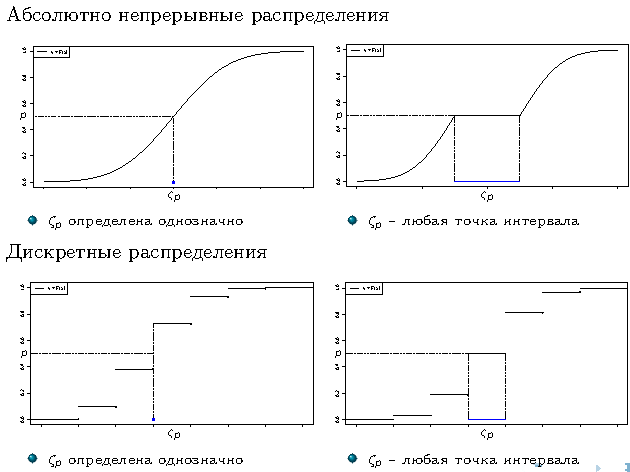
\includegraphics[scale=1.3]{./media/quantile.pdf}}
	\end{figure}
	Неформально можно определить квантиль, как значение, которое заданная случайная величина не превышает с фиксированной вероятностью.
\end{definition}

\begin{definition}[Критическая точка]
	Критической точкой порядка $\alpha$ распределения непрерывной случайной величины $\xi$ называется действительное число $t_{\alpha}$, удовлетворяющее уравнению $P(\xi \ge t_{\alpha}) = \alpha$.
	
	Очевидно, что квантиль порядка $\beta$ совпадает с критической точкой порядка $\alpha = 1 - \beta$, поскольку
	\[ P(\xi \ge t_{\alpha}) = 1 - P(\xi \le t_{\alpha}) = \alpha. \]
\end{definition}

\begin{definition}[Ковариация]
	Пусть $(\Omega, \Event, P)$ - вероятностный эксперимент, а $\xi, \eta$ - случайные величины, определённые в нём.
	
	Смешанный центральный момент второго порядка
	\[ E (\xi - E\xi) (\eta - E\eta) = \cov (\xi, \eta) \]
	называется ковариацией случайных величин $\xi$ и $\eta$.
	
	Для ковариации выполняются следующие свойства:
	\begin{enumerate}
		\item $\cov (\xi, \eta) = E \xi \eta - E \xi E \eta$;
		\item Если $\xi, \eta$ - независимые случайные величины, то $\cov (\xi, \eta) = 0$;
		
		Обратное утверждение — неверное.
		
		\item Если $a, b$ - числа, то $\cov (a \xi + b, \eta) = a \cov (\xi, \eta)$.
	\end{enumerate}
\end{definition}

\begin{definition}[Некоррелированные случайные величины]
	Если $\cov (\xi, \eta) = 0$, то такие случайные величины называют некоррелированными.
	
	Данное определение позволяет свойство 5 для дисперсии (см. раздел \ref{dispersion}) переформулировать следующим образом.
	
	\noindent 5'. Для некоррелированных случайных величин $\xi$ и $\eta$ справедливо равенство
	\[ D(\xi + \eta) = D\xi + D\eta \]
	В обратную сторону это утверждение также верно.
\end{definition}

\begin{definition}[Коэффициент корреляции]
	Пусть $\xi, \eta$ - случайные величины, у которых существуют дисперсии и $D\xi D\eta > 0$. Тогда число
	\[ \rho (\xi, \eta) = \frac{\cov (\xi, \eta)}{\sqrt{D\xi \cdot D\eta}} \]
	называется коэффициентом корреляции случайных величин $\xi$ и $\eta$.
\end{definition}

\begin{remark}
	Коэффициент корреляции можно записать и в следующей форме:
	\[ \rho (\xi, \eta) = E \frac{\xi - E \xi}{\sqrt{D \xi}} \cdot \frac{\eta - E\eta}{\sqrt{D \eta}} \]
	При этом заметим, что
	\[ E \frac{\xi - E\xi}{\sqrt{D \xi}} = E \frac{\eta - E \eta}{\sqrt{D \eta}} = 0, D \frac{\xi - E \xi}{\sqrt{D \xi}} \frac{D \xi}{D\xi} = 1, d \frac{\eta - E \eta}{\sqrt{D \eta}} \frac{D \eta}{D \eta} = 1 \]
	Таким образом, говорим, что мы провели \textit{центрирование} и \textit{нормирование} случайных величин. Получаем, что коэффициент корреляции совпадает с математическим ожиданием произведения центрированных и нормированных случайных величин.
\end{remark}

Для коэффициента корреляции выполняются следующие свойства.

\begin{enumerate}
	\item Справедливы неравенства:
	\[ -1 \le \rho (\xi, \eta) \le 1 (\text{т.е. } |\rho(\xi, \eta)| \le 1) \]
	\item Если $\xi, \eta$ - независимые случайные величины, то $\rho (\xi, \eta) = 0$. (Обратное утверждение - неверное.)
	\item Если $|\rho(\xi, \eta)| = 1$, то это означает, что существуют числа $a \ne 0$ и $b$ такие, что $P(\xi = a\eta + b) = 1$ (т.е. $\xi$ и $\eta$ - линейно связные с вероятностью единица величины), и $a \rho(\xi, \eta)>0$ (т.е. знак $a$ совпадает со знаком коэффициента корреляции).
\end{enumerate}

\begin{definition}[Матрица ковариации]
	Матрица ковариации - это матрица, составленная из попарных ковариаций элементов одного или двух случайных векторов.
	\[
	\vec{\xi} =
	\begin{pmatrix}
		r_{11} & \dots & r_{1n} \\
		\dots  & \dots & \dots \\
		r_{n1} & \dots & r_{nn}
	\end{pmatrix},
	r_{ij} = \cov (\xi_i, \xi_j)
	\]
	
	\textit{Ковариационная матрица случайного вектора} — квадратная симметрическая неотрицательно определенная матрица, на диагонали которой располагаются дисперсии компонент вектора, а внедиагональные элементы — ковариации между компонентами.
	
	Ковариационная матрица случайного вектора является многомерным аналогом дисперсии случайной величины для случайных векторов. Матрица ковариаций двух случайных векторов- многомерный аналог ковариации между двумя случайными величинами.
	
	В случае нормально распределенного случайного вектора, ковариационная матрица вместе с математическим ожиданием этого вектора полностью определяют его распределение (по аналогии с тем, что математическое ожидание и дисперсия нормально распределенной случайной величины полностью определяют её распределение).
\end{definition}

\begin{remark}
	Матрица корреляции - аналогично.
\end{remark}

\subsection{Случайные векторы}

Пусть $(\Omega, \mathcal{F}, P)$ - вероятностный эксперимент, в котором определено измеримое отображение $\xi: \Omega \to \mathbb{R}^d$. Говорим, что $\xi$ - измеримое отображение, если $\xi^{-1}(B) \in \mathcal{F}$ для любого множества $B \in \mathcal{B}^d$. Это отображение будем называть случайным вектором. Здесь $\mathbb{R}^d$ - $d$-мерное евклидово пространство, а $\mathcal{B}^d$ - сигма-алгебра борелевских подмножеств пространства $\mathbb{R}^d$.

Случайные векторы можно определить и несколько иначе. Пусть $\xi_1, \xi_2, \dots, \xi_d$ - случайные величины, определенные на одном и том же вероятностном пространстве. Определим отображение:
\[ \xi = (\xi_1, \xi_2, \dots, \xi_d) : \Omega \to \mathbb{R}^d \]
по правилу $\xi (\omega) = (\xi_1(\omega), \dots, \xi_d (\omega))$. Это и есть $d$-мерный случайный вектор.

Случайные векторы возникают, когда в результате эксперимента нас интересует сразу несколько характеристик наблюдаемого объекта. Как и для случайных величин, для случайного вектора можно определить функцию распределения.

\begin{definition}[Распределение случайного вектора]
\[\mathcal{P}_{\xi=(\xi_1,\dots,\xi_d)}(A)=P(\omega:f(\omega) \in A), A\in \Borel^n (A - \text{параллелепипед})\]
\end{definition}

\begin{definition}[Функция распределения случайного вектора]
	Функцию распределения случайного вектора $\xi = (\xi_1, \xi_2, \dots, \xi_d)$ определяем как функцию $F_{\xi}: \mathbb{R}^d \to \mathbb{R}^1$ такую, что для любого $(x_1, \dots, x_d) \in \mathbb{R}^d$
	\[ F_{\xi} (x_1, x_2, \dots, x_d) = P(\xi_1 < x_1, \xi_2 < x_2, \dots, \xi_d < x_d) \]

	\noindent Через распределение случайного вектора функция распределения выражается так:
	\[F_\xi(x_1,\dots,x_d) = \mathcal{P}_\xi((-\infty,x_1]\times(-\infty, x_n]))\]
\end{definition}

\begin{center}
	\textbf{Свойства функции распределения случайного вектора}
\end{center}
\begin{enumerate}
	\item $0 \le F_{\xi} (x_1, \dots, x_d) \le 1$.
	\item $F_{\xi}$ - непрерывна слева по каждой координате\footnote{Функция $f(x)$ называется непрерывной слева в точке $a$, если $f(a-0) = \lim\limits_{x \to a - 0} f(x) = f(a)$.}.
	\item $F_{\xi} (x_1, \dots, x_k, \dots, x_d) \underset{x_k \to - \infty}{\to} 0$, для любого $k \le d$.
	\item $F_{\xi} (x_1, \dots, x_k, \dots, x_d) \underset{x_k \to \infty}{\to} F_{(\xi_1, \dots, \xi_{k-1}, \xi_{x+1}, \dots, \xi_d)} (x_1, \dots, x_{k-1}, x_{k+1}, \dots, x_d)$, для любого $k \le d$, и
	
	$F_{\xi} (x_1, \dots, x_d) \to 1$, если одновременно все переменные $x_1, x_2, \dots, x_d$ стремятся к бесконечности.
	\item Пусть $d=2$ и пусть $a_1 < b_1, a_2 < b_2$. Тогда
	\[ P( (\xi_1, \xi_2) \in [a_1;b_1) \times [a_2;b_2) ) = F_{\xi} (b_1, b_2) - F_{\xi} (a_1, b_2) - F_{\xi} (b_1, a_2) + F_{\xi} (a_1, a_2) \]
\end{enumerate}

\subsubsection{Типы распределения случайных векторов}

\begin{definition}[Случайные векторы с дискретным законом распределением]
	Случайный вектор $\vec{\xi}$ имеет дискретное распределение, если существует такое не более чем счётное множество $A \subset \mathbb{R}^d$, что $P(\xi \in A) = 1$.
	
	Отметим, что следующие два утверждения равносильны:
	\begin{enumerate}
		\item $\xi = (\xi_1, \dots, \xi_d)$ - случайный вектор с дискретным распределением.
		\item Для всех $k \le d$ случайные величины $\xi_k$ имеют дискретное распределение.
	\end{enumerate}
\end{definition}

\begin{definition}[Случайный вектор с непрерывным законом распределения]
	Случайный вектор $\vec{\xi}$ называется непрерывным, если $F_{\xi}$ - непрерывная функция $n$ аргументов.
\end{definition}

\begin{definition}[Случайные векторы с абсолютно непрерывным законом распределения]
	Случайный вектор $\xi$ с абсолютно непрерывным распределением, если существует такая функция $p_{\xi} (x_1, x_2, \dots, x_d)$, что при любом $(y_1, y_2, \dots, y_d)$ справедливо равенство
	\[ F_{\vec{\xi}} (y_1, \dots, y_d) = \int_{-\infty}^{y_1} \dots \int_{-\infty}^{y_d} p_{\vec{\xi}} (x_1, \dots, x_d) dx_1 \dots dx_d = \int\limits_{( - \infty; y_1 ] \times \dots \times ( - \infty; y_n ]} p_{\vec{\xi}} (\vec{x}) d \mu_n (\vec{x}) \]
	Здесь функция $p_{\vec{\xi}}$ называется плотностью распределения случайного вектора, а $\mu_n$ - мера Лебега.
\end{definition}



\begin{center}
	\textbf{Распределение компонент случайного вектора}
\end{center}
\[ F_{\xi_i} = F_{\vec{\xi}} ( + \infty, \dots, + \infty, x, + \infty, \dots, + \infty ) = \lim\limits_{\underset{i \ne j}{x_j \to \infty}} F_{\vec{\xi}} (x_1, \dots, x_{i-1}, x, x_{i+1}, \dots, x_n) \]

\begin{center}
	\textbf{Свойства многомерных плотностей распределения}
\end{center}
\begin{enumerate}
	\item $p_{\xi} (x_1, \dots, x_n) \ge 0$ почти всюду.
	\item $\int\limits_{\mathbb{R}^n} p_{\xi} (x_1, x_2, \dots, x_n) dx_1 dx_2 \dots dx_n = 1$.
\end{enumerate}
Понятно, что для случайного вектора с абсолютно непрерывным распределением почти всюду выполняется равенство

\[ p_{\vec{\xi}} (x_1, \dots, x_n) = \dfrac{\partial^n}{\partial x_1 \dots \partial x_n} F_{\vec{\xi}} (x_1, \dots, x_n) \]
\[ (x_1, \dots, x_n) \in \mathbb{R}^n \]
Для дискретных величин:
\[ q_{\vec{\xi}} (\vec{a_i}) = P(\vec{\xi} = \vec{a_i}), \sum q (\underset{= \vec{a_i} = (a_{i_1}, \dots, a_{i_n})}{\vec{a_i}}) = 1 \]
\[ P(\xi_j = x_j) = \sum_{i: a_{ij} = x_j} q_{\vec{\xi}} (\vec{a_i}) \]

\begin{definition}[Непрерывное, но не абсолютно непрерывное распределение]
	\[ \eta \sim U(0, 1); ~~~ \xi_1 = \eta; ~~~ \xi_2 = 1 - \eta \]
	\[ F_{\vec{\xi}} (x, y) = P(\xi_1 < x, \xi_2 < y) = P(\eta < x, 1 - \eta < y) = P(1 - y < \eta < x) = \]
	\[
	\begin{cases}
		0, & x \le 0 \lor |y \le 0|, x + y - 1 \le 0 \\
		1, & x > 1, y > 1 \\
		x + y - 1, & x \le 1, y \le 1, x + y > 1 \\
		y, & x > 1, y \in (0, 1] \\
		x, & x \in [0, 1], y > 1
	\end{cases}
	\]
	\begin{figure}[H]
		\center{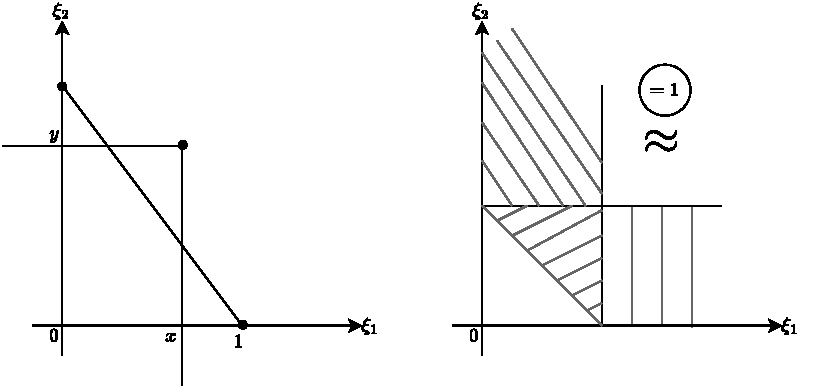
\includegraphics[scale=1.3]{./media/continuous_but_absolutely_continuous_distribution.pdf}}
	\end{figure}
\end{definition}

\subsubsection{Числовые характеристики случайных векторов}
\begin{figure}[H]
	\center{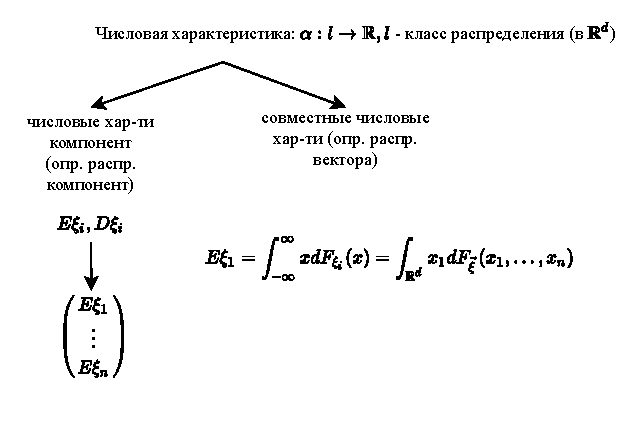
\includegraphics[scale=1.4]{./media/numerical_characteristics_of_random_vectors.pdf}}
\end{figure}

\begin{center}
	\textbf{Моментные характеристики}
\end{center}
\[ g: \mathbb{R}^n \to \mathbb{R} \]
\[ Eg (\xi_1 \dots \xi_n) = \int\limits_{\mathbb{R}^n} g (x_1 \dots x_n) d F(x_1, \dots, x_n) \]

Смотри ковариацию и коэффициент ковариации в разделе \ref{numerical_characteristics_of_random}.

\begin{exmp}
	\noindent\textit{\textbf{Условие:}}
	
	Случайный вектор $(\xi, \eta)$ имеет равномерное распределение в квадрате $[0,1] \times [0,1]$ с плотностью:
	\[
	p_{\xi, \eta} (x,y) =
	\begin{cases}
		1, x, y \in [0,1] \\
		0 - \text{ в остальных случаях}
	\end{cases}
	\]
	
	Найти распределение следующих комбинаций случайных величин:
	\begin{enumerate}
		\item[а)] $(\xi + \eta)^2$;
		\item[б)] $2 \xi + 3 \eta$;
		\item[в)] $\xi^2 + \eta^2$;
		\item[г)] $(\xi, \xi + \eta)$.
	\end{enumerate}
	
	\noindent\textit{\textbf{Решение:}}
	
	\begin{enumerate}
		\item[а)]
		
		Носитель распределения:
		\[ \supp (\xi) = \supp (\eta) = [0,1], (\xi + \eta)^2 < t \Rightarrow \xi + \eta < \sqrt{t}, 0 < t \le 4 \]
		Функция распределения:
		\[ F_{(\xi + \eta)^2} (t) = P( (\xi + \eta)^2 < t ) \]
		\begin{figure}[H]
			\center{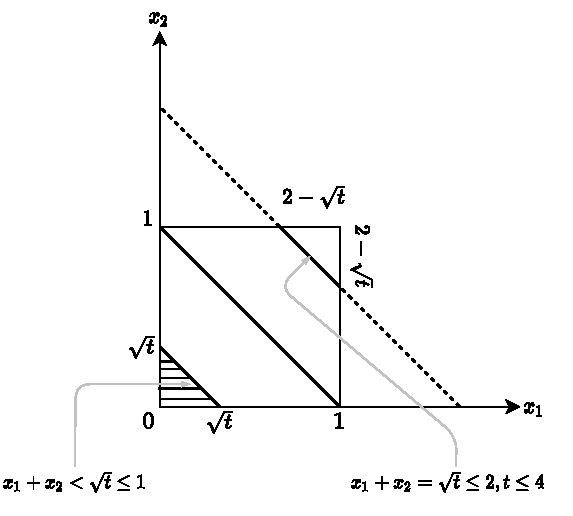
\includegraphics[scale=0.9]{./media/4_1.pdf}}
		\end{figure}
		
		Воспользуемся геометрическим определением интеграла для нахождения функции распределения данной случайной величины.
		
		При $t \in (0, 1]$ (площадь заштрихованной области):
		\[ F_{(\xi + \eta)^2} (t) = \int_{0}^{\sqrt{t}} dx_2 \int_{0}^{\sqrt{t} - x_2} dx_1 = \int_{0}^{\sqrt{t}} (\sqrt{t} - x_2) dx_2 = \frac{t}{2} \]
		
		При $t \in (1, 4]$ (вычитаем из площади квадрата $[0,1] \times [0,1]$ площадь треугольника со сторонами $2 - \sqrt{t}$):
		\[ F_{(\xi + \eta)^2} (t) = 1 - \int_{0}^{2 - \sqrt{t}} dx_2 \int_{0}^{2 - \sqrt{t} - x_2} dx_1 = \int_{0}^{2 - \sqrt{t}}(-\sqrt{t} - x_2 + 2) dx_2 = 1 - \frac{(\sqrt{r} - 2)^2}{2} \]
		Таким образом, функция распределения имеет следующий вид:
		\[
		F_{(\xi + \eta)^2} (t) =
		\begin{cases}
			0, &t \le 0 \\
			\frac{t}{2}, &t \in (0,1] \\
			1 - \frac{(\sqrt{t} - 2)^2}{2}, &t \in (1, 4] \\
			1, & t > 4
		\end{cases}
		\]
		График функции представлен ниже:
		\begin{figure}[H]
			\center{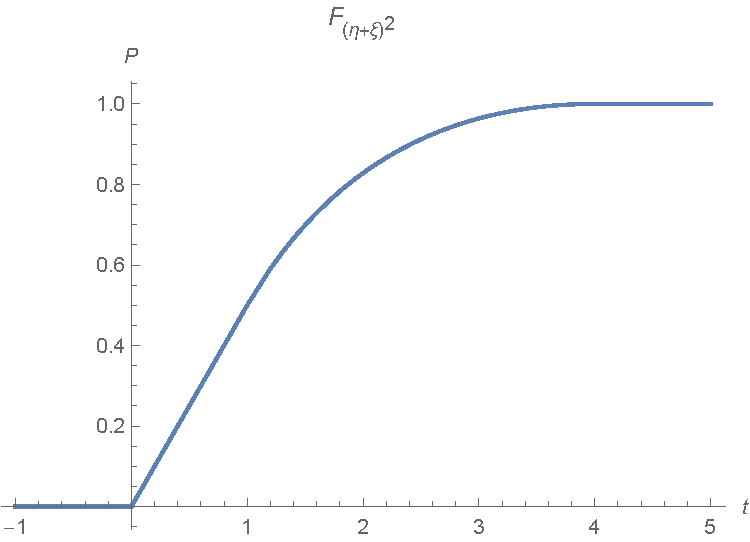
\includegraphics[scale=0.9]{./media/4_2.pdf}}
		\end{figure}
		\item[б)]
		
		Носитель распределения:
		\[ \supp (\xi) = \supp (\eta) = [0,1], 2\xi + 3 \eta < t, 0 < t \le 5 \]
		Функция распределения:
		\[ F_{2 \xi + 3 \eta} (t) = P(2 \xi + 3 \eta < t) \]
		Для удобства вычислений разобьём квадрат на несколько зон, а также введём несколько обозначений: $T_i$ - треугольник, используемый для вычислений в $i$-ой зоне; номера зон на рисунке помещены в синие рамки. \textcolor{Grey}{Границы интегрирования выражаются из носителя.}
		\begin{itemize}
			\item При $t \in (0, 2]$ функция распределения равна площади $T_1$, находящегося под прямой $2x_1+3x_2=t$:
			\[ F_{2\xi + 3\eta} (t) = \int_{0}^{\frac{t}{2}} dx_1 \int_{0}^{\frac{t-2x_1}{3}}dx_2 = \frac{t^2}{12} \]
			\item При $t \in (2, 3]$ функция распределения равна площади $T_1 - T_2$, где $T_2$ - площадь прямоугольника под вышеобозначенной прямой, но вне квадрата (зона 2).
			\[ F_{2\xi + 3\eta} (t) = \frac{t^2}{12} - \int_{0}^{\frac{t-2}{2}}dx_1 \int_{0}^{\frac{t-2x_1-2}{3}} dx_2 = \frac{t^2}{12} - \frac{1}{12} (t - 2)^2 = \frac{t-1}{3} \]
			\item При $t \in (3, 4]$ функция распределения равна разности площади квадрата и площади $T_3$, находящегося над прямой $2x_1 + 3x_2 = 4$ и образующего 4-ю область (находим 3-ю).
			\[ F_{2\xi + 3\eta} (t) = 1 - \int_{0}^{\frac{5-t}{2}}dx_1 \int_{0}^{\frac{5-2x_1-t}{3}} dx_2 = 1 - \frac{1}{12} (t - 5)^2 \]
		\end{itemize}
		\begin{figure}[H]
			\center{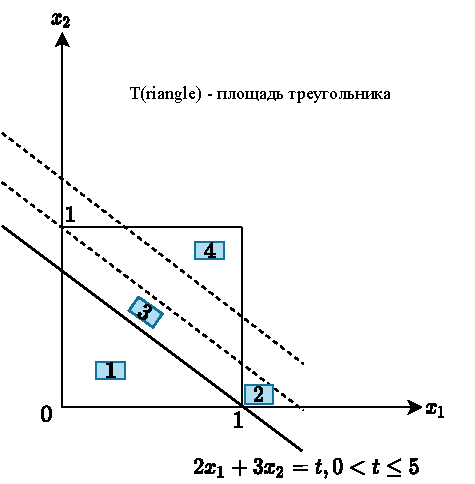
\includegraphics[scale=0.9]{./media/4_3.pdf}}
		\end{figure}
		Таком образом, функция распределения имеет следующий вид:
		\[
		F_{2\xi + 3\eta} (t) =
		\begin{cases}
			0, &t \le 0 \\
			\frac{t^2}{12}, &t \in (0, 2] \\
			\frac{t-1}{3}, &t \in (2, 3] \\
			1 - \frac{1}{12}(t-5)^2, &t \in (3, 5] \\
			1, &t > 5
		\end{cases}
		\]
		График функции представлен ниже:
		\begin{figure}[H]
			\center{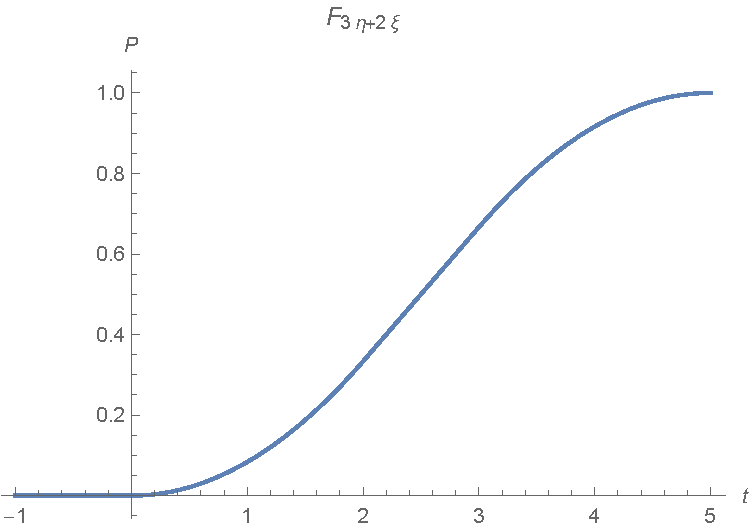
\includegraphics[scale=0.9]{./media/4_4.pdf}}
		\end{figure}
		
		\item[в)]
		Носитель распределения:
		\[ \supp (\xi) = \supp (\eta) = [0, 1], \xi^2 + \eta^2 < t, 0 < t < 2 \]
		Функция распределения:
		\[ F_{\xi^2 + \eta^2} = P(\xi^2 + \eta^2 < t) \]
		Заметим, что уравнение вида $x^2 + y^2 < z$ задаёт некоторую область внутри окружности радиуса $\sqrt{z}$ с центром в точке начала координат.
		
		Введём новое обозначение - $S_i$ - сектор, используемый в $i$-ой зоне.
		
		\begin{enumerate}
			\item[1.] При $t \in (0, 1]$ функция распределения равна площади сектора $S_1$, ограниченного прямыми координат и частью окружности с центром в $(0;0)$ и радиусом $t$. Требуемую площадь сектора найдём через следующую формулу:
			\[ S = \frac{\pi r^2 \alpha}{2 \pi} \]
			\[ F_{\xi^2 + \eta^2} (t) = \frac{t^2 \pi}{4} \]
			\item[2.] При $t \in (1, 2]$ функция распределения равна сумме прямоугольника со сторонами 1 и $\sqrt{t-1}$, а также криволинейной трапеции, образованной под прямой $x_1^2 + x_2^2 = t, x_1 = \sqrt{t-1} \dots t$ с основанием $1 - \sqrt{t-1}$.
			
			Очевидно, что площадь прямоугольника равна $\sqrt{t-1}$. Площадь же криволинейной трапеции (выражаем $x_2$):
			\[ \int_{\sqrt{t-1}}^{1} \sqrt{t-x_1^2} dx_1 = \frac{1}{2} \left( \sqrt{t-x^2} \cdot x + t \cdot \arcsin \frac{x}{\sqrt{t}} \right) \bigg|_{\sqrt{t-1}}^{1} = \]
			\[ = \dots = \frac{1}{2} t \left( \arcsin \frac{1}{\sqrt{t}} - \arcsin \frac{\sqrt{t-1}}{\sqrt{t}} \right) \]
		\end{enumerate}
		\begin{figure}[H]
			\center{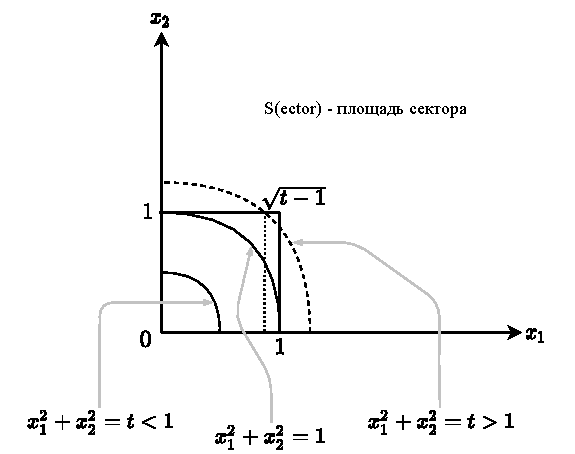
\includegraphics[scale=1.1]{./media/4_5.pdf}}
		\end{figure}
		Таким образом, функция распределения имеет следующий вид:
		\[
		F_{\xi^2 + \eta^2} (t) =
		\begin{cases}
			0, &t < 0 \\
			\frac{\pi t^2}{4}, &t \in (0, 1] \\
			\sqrt{t-1} + \frac{1}{2} t \left( \arcsin \frac{1}{\sqrt{t}} - \arcsin \frac{\sqrt{t-1}}{\sqrt{t}} \right), &t \in (1, 2] \\
			1, &t > 2
		\end{cases}
		\]
		График функции представлен ниже:
		\begin{figure}[H]
			\center{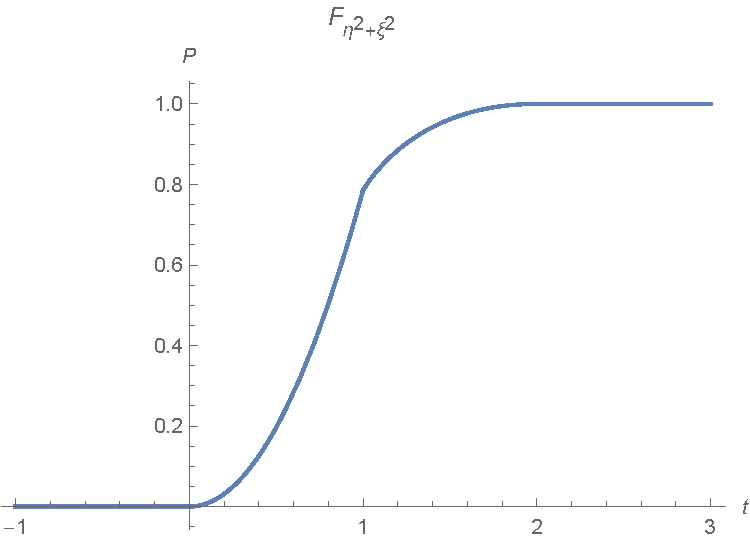
\includegraphics[scale=0.9]{./media/4_6.pdf}}
		\end{figure}
		
		Альтернативно,
		\[
		F_{\xi^2 + \eta^2} (t) =
		\begin{cases}
			0, &t < 0 \\
			\frac{\pi t^2}{4}, &t \in (0, 1] \\
			\sqrt{t-1} + \frac{t}{2} t \left( \arctan \frac{1}{\sqrt{t-1}} - \arctan (\sqrt{t-1}) \right), &t \in (1, 2] \\
			1, &t > 2
		\end{cases}
		\]
		Дифференцируем, преобразуем, находим плотность распределения
		\[
		p_{\xi^2 + \eta^2} =
		\begin{cases}
			\frac{\pi t}{2}, &t \in [0,1] \\
			\frac{1}{2} + \frac{\pi}{4} + \frac{1}{4 \sqrt{t-1}} - \arctan (\sqrt{t-1}), &t \in (1,2] \\
			1, &t > 2
		\end{cases}
		\]
		
		\textcolor{red}{(т.е. в окрестностях точек $t = 1$ и $t = 2$ функция распределения ведет себя не так как изображено
			на графике)}
		
		\item[г)]
		
		\[
		p_{\xi, \eta} (x, y) =
		\begin{cases}
			1, x, y \in [0, 1] \\
			0 - \text{ в остальных случаях}
		\end{cases}
		\]
		\[
		F_{\xi, \xi + \eta} (x_1, y_1) = P(\xi < x_1, \xi + \eta < y_1)
		\]
		\[
		\supp (x_1) = [0,1], ~~~ \supp (x_2) = [0,2]
		\]
		\begin{figure}[H]
			\center{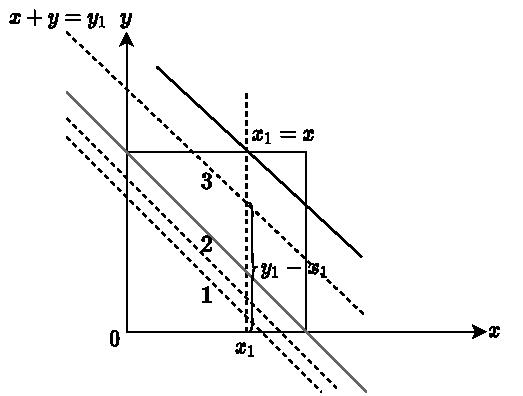
\includegraphics[scale=0.9]{./media/4_9.pdf}}
		\end{figure}
		
		На графике условие $x < x_1$ оставляет от квадрата прямоугольник от 0 до $x_1$ по оси $x$.
		
		Условие $x + y < y_1$ делает сечение прямоугольника, а итоговая фигура может быть либо треугольником (1 на рис.), либо трапецией (2 на рис.), либо прямоугольником с отсечённым треугольником (3 на рис.)
		
		Вычисляем функцию распределения $F_{\xi, \xi + \eta} (x, y)$ по областям (в скобках - форма области, площадь которой равна значению функции распределения).
		\begin{enumerate}
			\item $\{ x \le 0 \} \cup \{ y \le 0 \}$ (пустое множество): $F_{\xi, \xi + \eta} (x, y) = 0$;
			\item $\{ x \in (0, 1] \} \cap \{ 0 < y \le x \}$ (треугольник): $F_{\xi, \xi + \eta} (x, y) = P(\xi + \eta < y) = \frac{y^2}{2}$;
			\item $\{ x \in (0, 1] \} \cap \{ x < y \le x + 1 \}$ (трапеция): $F_{\xi, \xi + \eta} (x, y) = \left(y-\frac{x}{2}\right)x$;
			\item $\{ x \in (0, 1] \} \cap \{ y > x + 1 \}$ (прямоугольник): $F_{\xi, \xi + \eta} (x, y) = P(\xi < x) = x$;
			\item $\{ x > 1 \} \cap \{ y \in (0, 1] \}$ (треугольник): $F_{\xi, \xi + \eta} (x, y) = P(\xi + \eta < y) = \frac{y^2}{2}$;
			\item $\{ x > 1 \} \cap \{ y \in (1, 2] \}$ (прямоугольник с отсечённым треугольником): $F_{\xi, \xi + \eta} (x, y) = P(\xi + \eta < y) = 1 - \frac{(2-y)^2}{2}$;
			\item $\{ x > 1 \} \cap \{ y > 2 \}$ (квадрат $[0, 1]^2$): $F_{\xi, \xi + \eta} (x, y) = 1$.
		\end{enumerate}
		Таким образом,
		\[
		F_{\xi, \xi + \eta} (x, y) =
		\begin{cases}
			0, &x \le 0 \lor y \le 0 \\
			\frac{y^2}{2}, &x \in (0, 1], 0 < y \le x \lor x > 1, y \in (0, 1] \\
			\left( y - \frac{x}{2} \right) x, &x \in (0, 1], x < y \le x + 1 \\
			x, &x \in (0, 1], y > x + 1 \\
			1 - \frac{(2-y)^2}{2}, &x > 1, y \in (1, 2] \\
			1, &x > 1, y > 2
		\end{cases}
		\]
		Берем смешанную производную, получаем плотность распределения
		\[
		p_{\xi, \xi + \eta} (x, y) =
		\begin{cases}
			1, x \in [0, 1], x \le y \le x + 1 \\
			0 - \text{ в остальных случаях}
		\end{cases}
		\]
		
	\end{enumerate}
\end{exmp}

\subsection{Условные распределения}
Пусть $\xi = (\xi_1,\dots,\xi_n)$ - случайный вектор, $\xi = (\eta_1, \eta_2)$, где $\eta_1=(\xi_1,\dots,\xi_k), \eta_2=(\xi_{k+1},\dots,\xi_n)$.

Пусть $\eta_1=y$ - известен. Условное распределение $\eta_2$ при условии $\eta_1$?
\subsubsection{Дискретный случай}
\[a_i=(b_{1i}, b_{2i})\]
\[P(\eta_2=b_{2i} | \eta_1=b_{1i})=\dfrac{P(\xi=a_i)}{\underbrace{P(\eta_1=b_{1i})}_{>0}} = \dfrac{P(\eta_2=b_{2i}, \eta_1=b_{1i})}{\underbrace{P(\eta_1=b_{1i})}_{>0}} \]

\subsubsection{Абсолютно непрерывный случай}
Пусть $(\xi_1, \xi_2)$ - случайные величины (векторы), $p_{\vec{\xi}}(x,y)$ - плотность совместного распределения.

\[p_{\xi_1}(x)=\int_{-\infty}^{\infty} p_{\vec{\xi}}(x,y)dy \text{ - плотность распределения } \xi_1\]
\[p_{\xi_2|\xi_1=x}(y)=\dfrac{p_\xi(x,y)}{\underbrace{p_{\xi_1}(x)}_{>0}}, y\in \mathbb{R}, x \text{ - фиксированный}\]

\subsubsection{Условное мат. ожидание}
\[E(\xi_2|\xi_1=x)=\int_{-\infty}^{\infty} y \cdot p_{\xi_2|\xi_1=x}(y)dy = f(x) \text{ - зависит от значения фиксированного } x\]
Условное ожидание случайной величины $\xi_2$ относительно $\xi_1$:
\[E(\xi_2|\xi_1)=E(\xi_2|\xi_1=x)|_{\xi_1=x}=f(\xi_1) \text{ - то же самое, но зависит от } \xi_1\]

\begin{center}
	\textbf{Свойства условных мат. ожиданий}
\end{center}
\[f(\eta)=E(\xi|\eta)\]
\begin{enumerate}
	\item $E(E(\xi|\eta))=E\xi$
	\item Если $\xi, \eta$ - независимые, то $E(\xi|\eta)=E\xi$
	\item $E(g(\xi)|\xi)=g(\xi)$, если $g$ - фиксированная изначально функция
	\item $E(\xi\eta|\xi)=\xi E(\eta|\xi)$
	\item $E(\xi|\eta)=E(E(\xi|(\eta,\nu))|\eta), \forall \xi,\eta=E((E|\xi|\eta)|(\eta,\nu))$
\end{enumerate}

\subsubsection{Свойства условных распределений и их числовых характеристик}
\begin{definition}[Формула полной вероятности]
	Пусть $\xi_1, \xi_2$ - абсолютно непрерывные случайные величины на $(\Omega, \mathcal{F}, P)$ с совместной плотностью распределения $p_{\vec{\xi}}(x,y)$.

	\[\eta=\xi_1+\xi_2\]
	\[p_\eta(t)=\int_\mathbb{R} p_{\xi_1|\xi_2=y} (t-y) p_{\xi_2} (y)dy = \int_\mathbb{R} p_{\xi_2|\xi_1=x}(t-x) p_{\xi_1}(x)dx\]
	
	\noindent Если $\xi_1, \xi_2$ - независимы, то
	\[ p_{\vec{\xi}} (x, y) = p_{\xi_1} (x) p_{\xi_2} (y); ~~~~~~~~~ p_{\xi_1 | \xi_2} = y(x) = p_{\xi_1} (x) \]
	
	\noindent Отсюда можно получить формулу свёртки для плотностей:
	\[ p_{\eta} (t) = \int_{\mathbb{R}} p_{\xi_1} (t - y) p_{\xi_2} (y) dy = \int_{\mathbb{R}} p_{\xi_2} (t - x) p_{\xi_1} (x) dx \]
	
	\noindent Можно использовать и для других функций, например, $\eta = \xi_1 \xi_2$:
	\[ p_{\eta} (t) = \int_{\mathbb{R}} p_{\xi_1 | \xi_2 = y} \left( \frac{t}{y} \right) p_{\xi_2} (y) dy \]
\end{definition}

\begin{definition}[Формула свертки]
	Предположим, что $\xi, \eta$ - независимые случайные величины с известными нам функциями распределения $F_{\xi}, F_{\eta}$. Как вычислить $P(\xi + \eta \in D)$, где $D$ - произвольное измеримое подмножество вещественной прямой\footnote{Напомним, что борелевская сигма-алгебра - это минимальная сигма-алгебра, содержащая все открытые подмножества топологического пространства (впрочем, она содержит и все замкнутые). Обычно в качестве топологического пространства выступает множество вещественных чисел.}? Известно, что
	\[ P(\xi + \eta \in D) = \int_{D} d F_{\xi + \eta} (x) \]
	Следовательно, нам надо научиться находить функцию распределение суммы случайных величин.
	
	Рассмотрим случайный вектор $(\xi, \eta)$. Мы знаем его функцию распределения. Поскольку $\xi$ и $\eta$ независимы, то $F_{(\xi, \eta)} (x, y) = F_{\xi} (x) F_{\eta} (y)$. Тогда
	\[ F_{(\xi + \eta)} (t) = P(\xi + \eta < t) = P((\xi, \eta) \in A_t) = \int_{A_t} d F_{(\xi, \eta)} (x, y) = \int_{A_t} d (F_{\xi} (x) F_{\eta} (y)), \]
	где $A_t = \{ (x, y)\in \mathbb{R}^2 : x + y < t \}$.
	
	Последнее выражение вычисляем как повторный интеграл:
	\[ \int\limits_{A_t} d ( F_{\xi}(x) F_{\eta} (y) ) = \int\limits_{-\infty}^{\infty} \left( \int\limits_{-\infty}^{t-y} d F_{\xi} (x) \right) d F_{\eta} (y) = \int\limits_{-\infty}^{\infty} F_{\xi} (t - y) d F_{\eta} (y) \]
	Итак, получили\textit{ формулу для вычисления функции распределения суммы независимых случайных величин}, которую называют формулой свертки функций распределения.
	\begin{center}
		\textbf{Формула свертки для функций распределения}
	\end{center}
	\[ F_{\xi + \eta} (x) = \int\limits_{-\infty}^{\infty} F_{\xi} (x - y) d F_{\eta} (y) = \int\limits_{-\infty}^{\infty} F_{\eta} (x - y) d F_{\xi} (y) \]
\end{definition}
\begin{corollary}\leavevmode \vspace*{-\bigskipamount}\vspace*{-\medskipamount}
	\begin{enumerate}
		\item Пусть случайная величина $\xi$ с \textbf{абсолютно непрерывным распределением} (т.е. имеется соответствующая плотность распределения $p_{\xi} (x)$). Тогда сумма $\xi + \eta$ представляет собой случайную величину с абсолютно непрерывным распределением и её плотность распределения может быть вычислена с помощью равенства:
		\[ p_{\xi + \eta} (x) = \int\limits_{-\infty}^{\infty} p_{\xi} (x - y) d F_{\eta} (y) \]
		Получаем из основной формулы путём дифференцирования по $x$.
		\item Если $\xi, \eta$ - независимые случайные величины с абсолютно непрерывными распределениями, то $\xi + \eta$ является случайной величиной с абсолютно непрерывным распределением и её плотность может быть вычислена с помощью равенств
		\[ p_{(\xi + \eta)} (x) = \int\limits_{-\infty}^{\infty} p_{\xi} (x - y) p_{\eta} (y) dy = \int\limits_{-\infty}^{\infty} p_{\eta} (x - y) p_{\xi} (y) dy. \]
		Данная формула называется \textbf{формулой свертки для плотностей}.
	\end{enumerate}
\end{corollary}

\begin{remark}\leavevmode \vspace*{-\medskipamount}
	\begin{itemize}
		\item Если даже одна из двух независимых случайных величин имеет дискретное, а вторая — абсолютно непрерывное распределение, то их сумма тоже имеет абсолютно непрерывное распределение.
		\item Аналог формулы свертки для функций распределения работает для любых распределений (переход к повторному интегралу по мере), в частности, для непрерывных. 
		\item В случае формулы свертки для плотностей  распределения можно рассматривать по отношению к некоторой мере, в этом случае формула для плотностей распространяется на случай любой пары распределений с определенным выбором доминирующей меры (например, $dF_1+dF_2$), но меры, доминирующей все распределения, не существует.
	\end{itemize}
\end{remark}

\begin{exmp}
	Условное распределение зависит от значения $\xi_2$
	\begin{table}[H]
		\centering
		\begin{tabular}{|l|c|c||c|}
			\hline
			\multicolumn{1}{|c|}{\diagbox{$\xi_2$}{$\xi_1$}} & $-1$  & $1$   & $\Sigma$ \\ \hline
			$\xi_2 = -1$                                     & $1/4$ & $3/4$ & 1        \\ \hline
			$\xi_2 = 0$                                      & $1/2$ & $1/2$ & 1        \\ \hline
			$\xi_2 = 1$                                      & $1/2$ & $1/2$ & 1        \\ \hline
		\end{tabular}
	\end{table}
	\[
	q_{\xi_1 | \xi_2 = -1} (-1) = \frac{p(\xi_1 = -1, \xi_2 = -1)}{p(\xi_2 = -1)} = \frac{0.1}{0.4} = \frac{1}{4}
	~~~~~~
	q_{\xi_1 | \xi_2 = -1} (1) = \frac{p(\xi_1 = 1, \xi_2 = -1)}{p(\xi_2 = -1)} = \frac{0.3}{0.4} = \frac{3}{4}
	\]
	В частности, распределение $\xi_1$ при условии $\xi_2 = -1$:
	\begin{table}[H]
		\centering
		\begin{tabular}{|c|c|c||c|}
			\hline
			знач. $\xi_1$ & $-1$  & $1$   & $\Sigma$ \\ \hline
			усл. вер-ть   & $1/4$ & $3/4$ & $1$      \\ \hline
		\end{tabular}
	\end{table}
\end{exmp}

\begin{exmp}
	\[
	E(\xi_1 | \xi_2 = -1) = -1 \cdot \frac{1}{4} + 1 \cdot \frac{3}{4} = \frac{1}{2}; ~~~~~~ D(\xi_1 | \xi_2 = -1) = 1 - \left( \frac{1}{2} \right)^2 = \frac{3}{4};
	\]
	\[
	E(\xi_1 | \xi_2 = 0) = 0; ~~~ E(\xi_1 | \xi_2 = 1) = 0; ~~~ D(\xi_1 | \xi_2 = 1) = 1.
	\]
	Итак
	\[
	E(\xi_1 | \xi_2) =
	\begin{cases}
		\frac{1}{2}, \text{ если } \xi_2 = -1 \\
		0, \text{ в ост. случ.}
	\end{cases}
	- \text{ с. величина};
	~~~~~~
	D(\xi_1 | \xi_2) =
	\begin{cases}
		\frac{3}{4}, \text{ если } \xi_2 = -1 \\
		1, \text{ в ост. случ.}
	\end{cases}
	- \text{ с. величина};
	\]
	\begin{table}[H]
		\centering
		\begin{tabular}{|c|c|c||c|c|c|}
			\hline
			$E(\xi_1 | \xi_2)$ & $0$   & $1/2$ & $D(\xi_1 | \xi_2)$ & $3/4$ & 1     \\ \hline
			вер.               & $0.6$ & $0.4$ & вер.               & $0.4$ & $0.6$ \\ \hline
		\end{tabular}
	\end{table}
	Например, $p(\xi_2 = -1) = 0.4$
\end{exmp}

\section{Предельные теоремы}

\subsection{Моменты случайной величины}

Пусть $\xi$ - случайная величина и пусть $k \ge 0$.

\begin{definition}
	Введём несколько новых понятий:
	\begin{enumerate}
		\item \textit{Моментом} $k$\textit{-го} \textit{порядка} случайной величины называется число $E\xi^k$, если это число существует.
		\item Число $E(\xi - E\xi)^k$ называют \textit{центральным моментом} $k$\textit{-го} \textit{порядка} случайной величины $\xi$.
		\item Число $|\xi|^k$ - это \textit{абсолютный момент} $k$\textit{-ого} \textit{порядка} случайной величины $\xi$.
		\item Число $E|\xi - E\xi|^k$ - это \textit{центральный абсолютный момент} $k$\textit{-ого} \textit{порядка} случайной величины $\xi$.
		\item Число $E \xi_{1}^{p_1}\xi_{2}^{p_2} \dots \xi_{n}^{p_n}$ называется \textit{смешанным моментом порядка} $p$ случайных величин $\xi_1, \xi_2, \dots, \xi_n$.
	\end{enumerate}
\end{definition}

\begin{remark}
	Первые 4 момента (при фиксированном значении $k$) либо одновременно существуют, либо одновременно отсутствуют.
\end{remark}

\begin{remark}
	Если для всех $1 \le k \le n$ существует $E \xi_k^p$ (момент порядка $p$), то существуют и смешанные моменты порядка $p$ для $\xi_1, \xi_2, \dots, \xi_n$.
\end{remark}

\begin{center}
	\textbf{Неравенства (св-ва) для моментов}
\end{center}
\begin{enumerate}
	\item Пусть $0 \le k < n$ и существует момент $E\xi^n$. Тогда существует и момент $E\xi^k$.
	\begin{proof}
		Заметим, что всегда справедливо неравенство $|x|^k < |x|^n + 1$. Поэтому, если существует момент порядка $n$, то $E |\xi|^k < E |\xi|^n + 1 < \infty$.
	\end{proof}
	\item \textit{\textbf{Неравенство Гёльдера}}. Если $r, s > 0$ и $\frac{1}{r} + \frac{1}{s} = 1$, то
	\[ E |\xi \eta| \le (E|\xi|^r)^{\frac{1}{r}} ( ( E |\eta|^s )^{\frac{1}{s}} ) \]
	для любых случайных величин $\xi, \eta$ (если соответствующие моменты существуют).
	\begin{proof}
		\[ x^2 - 1, r > 1 ~~~~~~~~ r(x - 1) \le x^r - 1 \] 
		\begin{figure}[H]
			\center{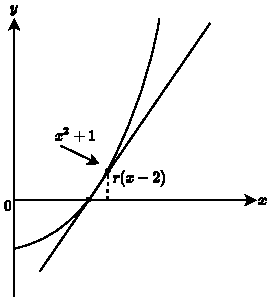
\includegraphics[scale=1.4]{./media/holder_inequality.pdf}}
		\end{figure}
		\[ x = \left( \frac{a}{b} \right)^{\frac{1}{r}} ~~~~~~~~ r \left( \left( \frac{a}{b} \right)^{\frac{1}{r}} - 1 \right) \le \frac{a}{b} - 1 \]
		\[ r \left( \frac{a^{\frac{1}{r}} - b^{\frac{1}{r}}}{b^{\frac{1}{r}}} \right) \le \frac{a - b}{b} ~~~~~~~~~ r (a^{\frac{1}{r}} b^{\frac{1}{r}} ) \le a - b \]
		\[ a^{\frac{1}{r}} b^{\frac{1}{r}} \le \frac{a}{r} + \frac{b}{s} \]
		\[ a = \frac{|\xi|^r}{E |\xi|^r} ~~~~~~~~~ b = \frac{|\eta|^2}{E|\eta|^2} \]
		\[ \Rightarrow \frac{|\xi| \cdot |\eta|}{(E |\xi|^r)^{\frac{1}{r}} (E |\eta|^s)^{\frac{1}{s}}} \le \frac{|\xi|^r}{r E |\xi|^r} + \frac{|\eta|^s}{s E |\eta|^s} \]
		\[ \Rightarrow \frac{E |\xi \eta|}{(E |\xi|^r)^{\frac{1}{r}} (E |\eta|^s)^{\frac{1}{s}}} \le \frac{\cancel{E |\xi|^r}}{r \cancel{E |\xi|^r}} + \frac{\cancel{E |\eta|^s}}{s \cancel{E |\eta|^s}} \]
		\[ \Rightarrow E |\xi \eta| \le (E |\xi|^r)^{\frac{1}{r}} (E |\xi|^s)^{\frac{1}{s}} \]
	\end{proof}
	\item[2.'] \textit{\textbf{Неравенство Коши–Буняковского–Шварца}} (частный случай неравенства Гёльдера при $p=q=2$). Если положим $p = q = 2$, то неравенство Гёльдера будет иметь следующий вид:
	\[ E |\xi \eta| \le ( E |\xi|^2 )^{\frac{1}{2}} \cdot ( E |\eta|^2 )^{\frac{1}{2}} \]
	\item \textit{\textbf{Неравенство Ляпунова.}} Если $p < q$, то $(E |\xi|^p)^{\frac{1}{p}} \le (E |\xi|^q)^{\frac{1}{q}}$. (Это свойство можно сформулировать иначе: введем функцию $g_{\xi}(p) = (E |\xi|^p)^{\frac{1}{2}}$, тогда $g_{\xi}(p)$ не убывает).
	\begin{proof}
		Верно равенство: $\frac{p}{q} + \frac{(q-p)}{q} = 1$. Воспользуемся неравенством Гёльдера, в котором вторая случайная величина имеет вырожденное в единице распределение. Сразу получим нужный результат:
		\[ E(|\xi|^p \cdot 1) \le (E(|\xi|^p)^{\frac{q}{p}})^{\frac{p}{q}} \cdot (E1^{\frac{q}{q-p}})^{\frac{q-p}{q}} = (E|\xi|^q)^{\frac{p}{q}} \]
	\end{proof}
	\item \textit{\textbf{Неравенство Минковского.}} Если $p, q > 0$ и $\frac{1}{p} + \frac{1}{q} = 1$, то
	\[ ( E |\xi + \eta|^p )^{\frac{1}{p}} \le ( E |\xi|^p )^{\frac{1}{p}} + ( E |\eta|^p )^{\frac{1}{p}} \]
	для любых случайных величин $\xi, \eta$.
	\begin{proof}
		Заметим, что в силу неравенства $|\xi + \eta| \le |\xi| + |\eta|$ выполняется
		\[ E |\xi + \eta|^p \le E |\xi| |\xi + \eta|^{p-1} + E |\eta| |\xi + \eta|^{p-1} \]
		Применяя здесь к слагаемым правой части неравенство Гёльдера, получим
		\[ E |\xi + \eta|^p \le ( ( E |\xi|^p )^{\frac{1}{p}} + ( E |\eta|^p )^{\frac{1}{p}} ) ( E |\xi + \eta|^{(p-1)q} )^{\frac{1}{q}} \]
		Так как $(p-1)q=p, 1=\frac{1}{q}=\frac{1}{p}$, то отсюда следует неравенство Минковского.
	\end{proof}
	\item \textit{\textbf{Неравенство Йенсена.}} Если $E\xi$ существует и $g(x)$ - выпуклая вниз функция, то $g(E\xi) \le E g(\xi)$.
	\begin{proof}
		Если $g(x)$ - выпуклая вниз, то для каждого $y$ найдется число $g^1(y)$ такое, что
		\[ g(x) \ge g(y) + (x-y)g^1(y) \]
		Положив здесь $x=\xi, y = E\xi$ и взяв математическое ожидание обеих частей этого неравенства, получим
		\[ Eg(\xi) \ge g(E\xi) \]
	\end{proof}
	\item \textit{\textbf{Неравенство Маркова.}} Для любого $t > 0$ и любой неотрицательной случайной величины $\xi$ справедливо неравенство:
	\[ P(\xi \ge t) \le \frac{E\xi}{t} \]
	\begin{proof}
		Рассмотрим
		\[ E\xi = \int\limits_{\Omega} \xi (\omega) d P(\omega) = \int\limits_{\omega : \xi (\omega) < t} \xi (\omega) d P(\omega) + \int\limits_{\omega : \xi (\omega) \ge t} \xi (\omega) d P(\omega) \ge \]
		\[ \ge \int\limits_{\omega : \xi (\omega) < t} \xi (\omega) d P(\omega) \ge t \int\limits_{\omega : (\omega) \ge t} d P (\omega) = t P(\ge t). \]
		Последнее равенство справедливо, поскольку
		\[ \int\limits_{\omega : \xi (\omega) \ge t} d P(\omega) = P (\xi \ge t). \]
	\end{proof}
	\begin{corollary}\leavevmode \vspace*{-\bigskipamount}\vspace*{-\medskipamount}
		\begin{enumerate}
			\item Пусть функция $f : \mathbb{R} \to \mathbb{R}$ обладает следующими свойствами: $f$ - чётная, $f(0) \ge 0$ и $f$ не убывает на $[0; \infty)$. Тогда для любого $t > 0$ справедливо неравенство
			\[ P ( |\xi - E\xi| \ge t ) \le \frac{E f(\xi - E \xi)}{f(t)} \]
			\begin{proof}
				\[ P ( |\xi - E \xi| \ge t ) = P ( f ( |\xi - E\xi| ) \ge f(t) ) = \]
				\[ = P ( f (\xi - E\xi) \ge f(t) ) \le \frac{Ef(\xi - E\xi)}{f(t)} \]
			\end{proof}
			\item Пусть у случайной величины $\xi$ существует дисперсия $D\xi$. Тогда для любого $t>0$ имеет место следующее неравенство Чебышёва (также см. след. пункт нер-в, где оно получается через неравенство Йенсена ($\epsilon$ - это $t$)).
			\[ P ( |\xi - E\xi| \ge t ) \le \frac{D\xi}{t^2} \]
			которое получается из предыдущего следствия, если взять $f(t) = t^2$.
		\end{enumerate}
	\end{corollary}
	\item \textit{\textbf{Неравенство Чебышева.}} Для произвольной случайной величины $\xi$, имеющей математическое ожидание, справедливо неравенство
	\[ P( |\xi - E\xi| \ge \epsilon ) \le \frac{D\xi}{\epsilon^2} \]
	при $D\xi < \infty$ и $\xi > 0$.
	
	\begin{proof}
		Для доказательства достаточно применить неравенство Йенсена к случайной величине $\eta = (\xi - E\xi)^2 \ge 0$.
	\end{proof}
	
	\noindent \textbf{Применение:}
	
	\begin{itemize}
		\item С помощью неравенства Чебышева мы имеем возможность оценивать вероятности различных уклонений $\xi$ (от мат. ожидания), зная лишь $E\xi$ и $D\xi$.
		\item Из данного нер-ва можно получить так называемый закон больших чисел в форме Чебышева.
	\end{itemize}
	
	\noindent Другая форма записи нер-ва Чебышева (используется реже):
	
	\[ g: \mathbb{R}_{+} \to \mathbb{R}_{+} - \text{ неотрицательная, неубывающая функция} \]
	\[ \text{Случайная величина } \xi : P(\xi > 0) = 1, ~~~~~~ Eg(\xi) < \infty, g(x) > 0, x > 0 \]
	\[ P (|\xi| > \epsilon) \le \frac{Eg(\xi)}{g(\xi)} \]
	\[ P( |\xi - E\xi| \ge \epsilon ) \le \frac{D\xi}{\epsilon^2} \]
\end{enumerate}

\subsection{Закон больших чисел и сходимость по вероятности}

\begin{definition}[Закон больших чисел (ЗБЧ)]
	Пусть $\xi_1, \xi_2, \dots$ - последовательность случайных величин, с математическими ожиданиями $a_k = E\xi_k, k = 1, 2, \dots$. Будем говорить, что для последовательности случайных величин выполняется закон больших чисел, если имеет место сходимость
	\[ \frac{1}{n} \sum_{k=1}^{n} (\xi_k - a_k) \overset{P}{\to} 0 \]
	Это означает, что
	\[ P \left( \left| \frac{1}{n} \sum_{k=1}^{n} \xi_k - \frac{1}{n} \sum_{k=1}^{n} a_k \right| \ge \epsilon \right) \underset{n \to \infty}{\to} 0 \]
	или, что то же самое,
	\[ P \left( \left| \frac{1}{n} \sum_{k=1}^{n} (\xi_k - a_k) \right| \ge \epsilon \right) \underset{n \to \infty}{\to} 0 \]
	для любого $\epsilon > 0$.
\end{definition}
\begin{remark}
	Выполнение ЗБЧ для последовательности $\xi_1, \xi_2, \dots$ равносильно выполнению ЗБЧ для последовательности $\xi_1 + b_1, \xi_2 + b_2, \dots,$ где $b_1, b_2, \dots$ - произвольные числа.
\end{remark}

ЗБЧ утверждает, что среднее значение случайных величин из заданного распределения близко к теоретическому среднему значению (математическое ожидание) этого распределения

На неформальном языке закон можно трактовать так: при увеличении числа испытаний частота появления события будет все меньше отличаться от вероятности его появления.

Установим условия, которым должны отвечать последовательности случайных величин, чтобы ЗБЧ выполнялся. Отметим, что приведённые теоремы указывают лишь достаточные условия.

\begin{theorem}[ЗБЧ Маркова]
	Пусть $\xi_1, \xi_2, \dots$ - случайные величины и пусть при всех $n \ge 1$ существуют дисперсии $D \left( \sum\limits_{k=1}^{n} \xi_k \right)$. Кроме того, пусть
	\[ \frac{1}{n^2} D \left( \sum\limits_{k=1}^{n} \xi_k \right) \underset{n \to \infty}{\to} 0 \]
	Тогда для данной последовательности выполняется закон больших чисел.
	\begin{proof}
		Применяя неравенство Чебышёва, получаем, что
		\[
		P \left( \left| \frac{1}{n} \sum_{k=1}^{n} \xi_k - E \frac{1}{n} \sum_{k=1}^{n} \xi_k \right| \ge \epsilon \right) \le \frac{D \left( \frac{1}{n} \sum\limits_{k=1}^{n} \xi_k \right)}{\epsilon^2} = \frac{D \left( \sum\limits_{k=1}^{n} \xi_k \right)}{n^2 \epsilon^2} \underset{n \to \infty}{\to} 0
		\]
	\end{proof}
\end{theorem}

\begin{theorem}[ЗБЧ Чебышёва]
	Пусть $\xi_1, \xi_2, \dots$ - попарно независимые случайные величины и пусть для всех $k = 1, 2, \dots$ существуют и равномерно ограничены дисперсии случайных величин, т.е. $\sigma_k^2 = D\xi_k \le c$, где $c$ - некоторая неотрицательная константа. Тогда для данной последовательности случайных величин выполняется закон больших чисел.
	\begin{proof}
		Утверждение сразу следует из теоремы Маркова, если учесть, что в данной ситуации
		\[ \frac{1}{n^2} D \left( \sum_{k=1}^{n} \xi_k \right) = \frac{1}{n^2} \sum_{k=1}^{n} \sigma_k^2 \le \frac{n \cdot c}{n^2} \underset{n \to \infty}{\to} 0 \]
	\end{proof}
\end{theorem}

\begin{corollary}[из теоремы Чебышёва]
	
	1. Если $\xi_1, \xi_2, \dots$ - независимые одинаково распределенные случайные величины и при всех $k \ge 1$ существуют дисперсии $D\xi = \sigma^2 > 0$, то выполняется ЗБЧ.
	
	\noindent 2. Пусть $\xi_1, \xi_2, \dots$ - независимые одинаково распределенные случайные величины, принимающие значения 0 и 1 с вероятностями $(1-p)$ и $p$, соответственно. Тогда
	\[ \frac{1}{n} \sum_{k-1}^{n} \xi_k \overset{P}{\to} p \]
	
	Заметим, что следствие 2 можно рассматривать как теорему о законе больших чисел для испытаний Бернулли.
\end{corollary}

\begin{theorem}[ЗБЧ Хинчина]
	Пусть $\xi_1, \xi_2, \dots$ - последовательность независимых одинаково распределенных случайных величин, у которых существует математическое ожидание $a = E \xi_k$. Тогда, для этой последовательности выполнен закон больших чисел, то есть
	\[ \frac{1}{n} \sum\limits_{k = 1}^{n} (\xi_k - a) \overset{P}{\to} 0 \]
	\begin{proof}
		Докажем сначала более слабую сходимость, а именно, сходимость по распределению:
		\[ \frac{1}{n} \sum\limits_{k = 1}^{n} (\xi_k - a) \overset{d}{\to} 0 \]
		Поскольку у случайных величин $\xi_k$ имеется математическое ожидание и $E (\xi_k - a) = 0$, то, согласно следствию из теоремы о связи гладкости характеристических функций с существованием моментов у случайной величины, имеет место соотношение
		\[ f_{\xi_{k-a}} (t) = 1 + \bar{o} (t) \]
		Из свойств характеристических функций имеем
		\[ f_{\frac{1}{n} \sum\limits_{k=1}^{n} (\xi_k - a)} (t) = f_{\sum\limits_{k=1}^{n}(\xi_k - a)} \left( \frac{t}{n} \right) = \left( f_{\xi_1 - a} \left( \frac{t}{n} \right) \right)^{n} = \left( 1 + \bar{o} \left( \frac{t}{n} \right) \right)^{n} \underset{n \to \infty}{\to 1} \]
		Это означает слабую сходимость функций распределения, то есть
		\[ P \left( \frac{1}{n} \sum_{k=1}^{n} (\xi_k - a) < x \right) \underset{n \to \infty}{\to} \begin{cases} 0, & x < 0 \\ 1, & x > 0 \end{cases} \]
		Таким образом, мы показали сходимость по распределению, а нам, все-таки, нужна сходимость по вероятности. Получим ее:
		\[ P \left( \left| \frac{1}{n} \sum_{k=1}^{n} ( \xi_k - a ) \right| \ge \epsilon \right) \le P \left( \frac{1}{n} \sum_{k=1}^{n} ( \xi_k - a ) \ge \epsilon \right) + P \left( \frac{1}{n} \sum_{k=1}^{n} ( \xi_k - a ) < - \epsilon \right) = \]
		\[ = 1 - P \left( \frac{1}{n} \sum_{k=1}^{n} ( \xi_k - a ) < \epsilon \right) + P \left( \frac{1}{n} \sum_{k=1}^{n} ( \xi-k - a ) < - \epsilon \right) \underset{n \to \infty}{\to} 0 \]
	\end{proof}
\end{theorem}

\begin{theorem}[Закон больших чисел Бернулли]
	Пусть $p = P(\text{'у'})$ - вероятность успеха в одном испытании, $\mu_n$ - число успехов в $n$ испытаниях. Тогда для любого положительного $\epsilon$ выполняется предельное соотношение:
	\[ P \left( \left| \frac{\mu_n}{n} - p \right| > \epsilon \right) \underset{n \to \infty}{\to} 0 \]
	(Отношение $\frac{\mu_n}{n}$ принято называть частотой успеха).
	\begin{proof}
		Видим, что
		\[ P \left( \left| \frac{\mu_n}{n} - p \right| > \epsilon \right) = 1 - P \left( \left| \frac{\mu_n}{n} - p \right| \le \epsilon \right) = \]
		\[ = \frac{1}{\sqrt{2 \pi}} \int_{- \infty}^{\infty} e^{-\frac{u^2}{2}} du - P \left( - \epsilon \sqrt{\frac{n}{pq}} \le \frac{\mu_n - np}{\sqrt{npq}} \le \epsilon \sqrt{\frac{n}{pq}} \right) = \]
		\[ = \frac{1}{\sqrt{2 \pi}} \int\limits_{|u| > \epsilon \sqrt{\frac{n}{pq}}} e^{-\frac{u^2}{2}} du + \frac{1}{\sqrt{2 \pi}} \int\limits_{|u| \le \epsilon \sqrt{\frac{n}{pq}}} e^{- \frac{u^2}{2}} du - P \left( - \epsilon \sqrt{\frac{n}{pq}} \le \frac{\mu_n - np}{\sqrt{npq}} \le \epsilon \sqrt{\frac{n}{pq}} \right) \underset{n \to \infty}{\to} 0, \]
		так как
		\[ \frac{1}{\sqrt{2 \pi}} \int\limits_{|u| > \epsilon \sqrt{\frac{n}{pq}}} e^{- \frac{u^2}{2}} du \underset{n \to \infty}{\to} 0 \]
		как "хвост" сходящегося интеграла, и
		\[ \frac{1}{\sqrt{2 \pi}} \int\limits_{|u| \le \epsilon \sqrt{\frac{n}{pq}}} e^{- \frac{u^2}{2}} du - P \left( - \epsilon \sqrt{\frac{n}{pq}} \le \frac{\mu_n - np}{\sqrt{npq}} \le \epsilon \sqrt{\frac{n}{pq}} \right) \underset{n \to \infty}{\to} 0 \]
		по интегральной предельной теореме Муавра—Лапласа.
	\end{proof}
\end{theorem}

\subsection{Сходимость последовательностей случайных величин}

Пусть $(\Omega, \mathcal{F}, P)$ - вероятностый эксперимент, на котором определены случайные величины $\xi, \xi_1, \xi_2, \dots$. Для последовательностей случайных величин можно рассматривать различные виды сходимостей. Ниже определим несколько из них.

\begin{enumerate}
	\item \textbf{Сходимость по вероятности.}
	
	Будем говорить, что последовательность случайных величин $\xi, \xi_1, \xi_2, \dots$ сходится к случайной величине $\xi$ по вероятности (обозначение: $\xi_n \overset{P}{\to} \xi$), если
	\[ P(|\xi_n - \xi| \ge \epsilon) \underset{n \to \infty}{\to} 0 \]
	для любого $\epsilon > 0$.
	
	\begin{exmp}[сходимости по вероятности]
		Рассмотрим последовательность $\xi_1, \xi_2, \dots$, в которой все величины имеют разные распределения: величина $\xi_n$ принимает значение $0$ и $n^7$ с вероятностями
		\[ P(\xi_n = n^7) = \frac{1}{n} = 1 - P(\xi_n = 0) \]
		Докажем, что эта последовательность сходится по вероятности к нулю.
		
		Зафиксируем произвольное $\epsilon > 0$. Для всех $n$, начиная с некоторого $n_0$ такого, что $n_{0}^{7} > \epsilon$, верно равенство $P(\xi_n \ge \epsilon) = P(\xi_n = n^7) = \frac{1}{n}$. Поэтому
		\[ P ( |\xi_n - 0| \ge \epsilon ) = P ( \xi_n \ge \epsilon ) = P ( \xi_n = n^7 ) = \frac{1}{n} \to 0 \text{ при } n \to \infty \]
		
		Итак, случайные величины $\xi_n$ с ростом $n$ могут принимать всё большие и большие значения, но со всё меньшей и меньшей вероятностью.
		
		Например, последовательность $\{ \xi_n \}$ можно задать на вероятностном пространстве $(\Omega, \Event, P) = ( [0, 1], \Borel([0, 1]), \lambda )$ так:
		\begin{figure}[H]
			\center{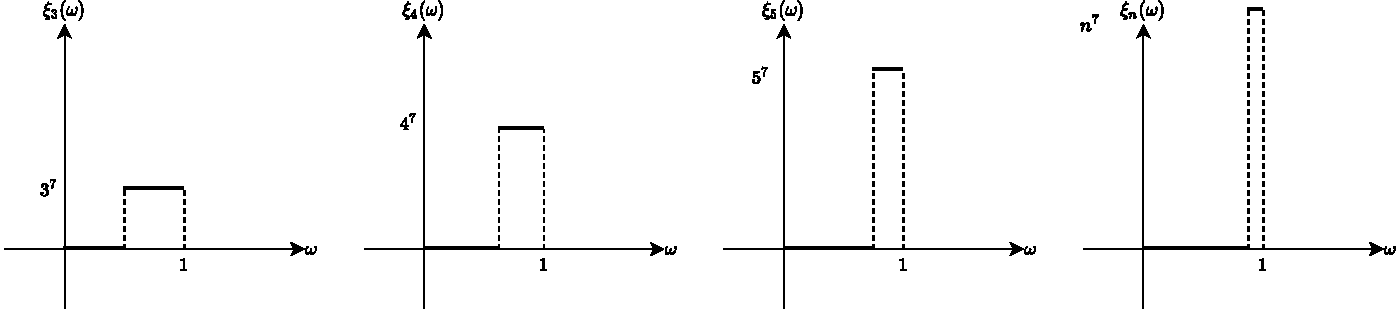
\includegraphics[scale=0.8]{./media/probability_convergence_exmp.pdf}}
		\end{figure}
		А именно, положим $\xi_n (\omega) = 0$ для $\omega \in \left[ 0, 1 - \frac{1}{n} \right]$ и $\xi_n (\omega) = n^7$ для $\omega \in \left( 1 - \frac{1}{n}, 1 \right]$. Заметим, что в данном случае (сходимости к постоянной) \textit{сходимость по вероятности имеет место совершенно независимо от того, как именно заданы случайные величины на} $\Omega$, поскольку определяется лишь их распределениями.
	\end{exmp}
	
	\item \textbf{Сходимость с вероятностью 1 или почти наверное.}
	
	Будем говорить, что последовательность случайных величин $\xi_1, \xi_2, \dots$ сходится к случайной величине $\xi$ почти наверное или с вероятностью 1 (обычно обозначается $\xi_n \to \xi$ п.н.), если верно равенство
	\[ P(\omega : \lim \xi_n (\omega) = \xi (\omega)) = 1 \]
	
	\begin{exmp}[сходимости почти наверное]
		Если, скажем, задать случайные величины как показано на графиках, то сходимость «почти наверное»  будет иметь место. Действительно, для всякого $\omega \in [0, 1)$ найдётся такое $n_0$, что $\omega \in \left[ 0, 1 - \frac{1}{n_0} \right]$, и поэтому для всех $n \ge n_0$ все $\xi_n (\omega)$ равны нулю.
		
		Можно попробовать задать случайные величины $\xi_n$ на $[0, 1]$ как-нибудь иначе, чтобы \textit{не было} сходимости \textit{почти наверное}. Для этого нужно заставить отрезок длины $\frac{1}{n}$, на котором $\xi_n (\omega) = n^7$, «бегать» по отрезку $[0, 1]$, чтобы любая точка $\omega \in [0, 1]$ попадала внутрь этого отрезка бесконечное число раз, и, тем самым, для любого $\omega$ существовала подпоследовательность $\xi_{n_k} (\omega) \to \infty$.
		
		Однако заметим, что если вероятности $P(\xi_n = n^7)$ сходятся к нулю достаточно быстро (например, равны $\frac{1}{n^2}$ - чтобы ряд из них сходился), то сходимость п.н. к нулю всегда имеет место.
	\end{exmp}
	
	\item \textbf{Сходимость в среднем порядкe} $p(p > 0)$
	
	Будем говорить, что последовательность случайных величин $\xi_1, \xi_2, \dots$ сходится к случайной величине $\xi$ в среднем порядка $p$ (обозначение: $\xi_n \overset{L_p}{\to} \xi$), если существует $E\xi^p$ и $E\xi_n^p$ и имеет место сходимость:
	\[ E |\xi - \xi_n|^p \underset{n \to \infty}{\to} 0 \]
	
	\item \textbf{Сходимость по распределению.}
	
	Будем говорить, что последовательность случайных величин $\xi_1, \xi_2, \dots$ сходится к случайной величине $\xi$ по распределению (обозначение: $\xi_n \overset{d}{\to} \xi$), если
	\[ F_{\xi_n} (x) \underset{n \to \infty}{\to} F_{\xi} (x) \]
	для любой $x$ - точки непрерывности функции $F_{\xi}$.
\end{enumerate}
\begin{remark}
	В пункте 4 сходятся не случайные величины, а их функции распределения. При этом случайные величины могут быть далеки друг от друга.
\end{remark}

\begin{exmp}[сходимости по распределению]
	Рассмотрим ситуацию, когда $\Omega = \{ \omega_1, \omega_2 \}, P( \{ \omega_1 \} ) = P( \{ \omega_2 \} ) = \frac{1}{2}, \xi ( \omega_1 ) = 0, \xi ( \omega_2 ) = 1, \xi_n = ( \omega_1 ), \xi_n ( \omega_2 ) = 0, n = 1, 2, \dots$
	
	Тогда $| \xi (\omega_i) - \omega_n (\omega_i) | = 1$ для всех элементарных исходов, т.е. и для $\omega_1$ и для $\omega_2$, но $F_{\xi} (x) = F_{\xi_n} (x)$ для всех $x \in \mathbb{R}$, и таким образом имеет место сходимость по распределению $\xi_n \overset{d}{\to} \xi$.
\end{exmp}

\begin{theorem}[О соотношениях между видами сходимостей]
	Имеют место следующие соотношения:
	\[ 2 \Rightarrow 1, 3 \Rightarrow 1, 1 \Rightarrow 4, \]
	т.е. из сходимости почти наверное следует сходимость по вероятности, из сходимости в среднем следует сходимость по вероятности и из сходимости по вероятности следует сходимость по распределению.
	\begin{figure}[H]
		\center{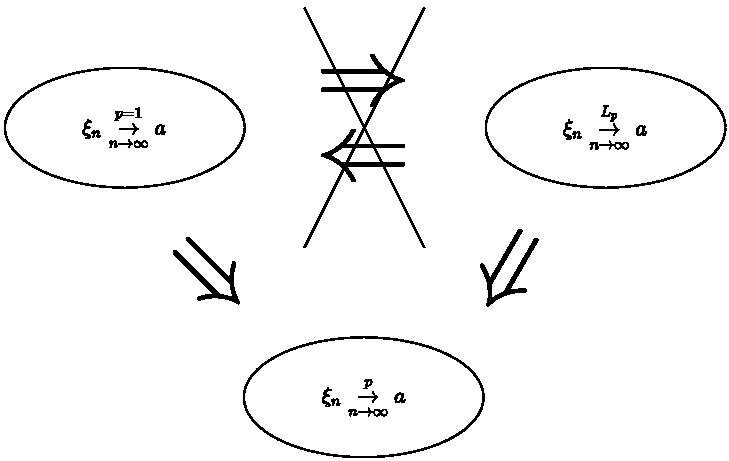
\includegraphics[scale=1]{./media/relationship_between_convergence.pdf}}
	\end{figure}
\end{theorem}

\subsection{Сходимость почти наверное и усиленный закон больших чисел}

Рассмотрим последовательность случайных событий $\{ A_n \}$ из одного и того же вероятностного пространства. Определим событие $A = $ (происходит бесконечное число из событий $A_n$).

Это означает следующее: $\omega \in A$ тогда и только тогда, когда $\omega$ принадлежит бесконечному числу событий $A_n$. Тогда имеет место следующее представление
\[ A = \bigcap_{n=1}^{\infty} \bigcup_{k=n}^{\infty} A_k \]

\textit{Следующие высказывания эквивалентны:}

\begin{enumerate}
	\item $\xi_n \to \xi$ почти наверное;
	\item $P(|\xi_n - \xi| > \epsilon$ бесконечное число раз) = 0 при любом $\epsilon > 0$;
	\item $P \left( \bigcap\limits_{n=1}^{\infty} \bigcup\limits_{k=n}^{\infty} (|\xi_k - \xi| > \epsilon) \right)$ при любом $\epsilon > 0$;
	\item Для любого $\epsilon > 0 \lim\limits_{n \to \infty} P(\sup\limits_{m \ge n} |\xi_m - \xi| > \epsilon) = 0$.
\end{enumerate}

\begin{lemma}[Бореля—Кантелли]
	Пусть $A_1, A_2, \dots$ - последовательность случайных событий и положим событие $A = \bigcap\limits_{n=1}^{\infty} \bigcup\limits_{k=n}^{\infty} A_k $. Справедливы два следующих утверждения.
	\begin{enumerate}
		\item Если $\sum\limits_{n=1}^{\infty} P(A_n) < \infty$, то $P(A) = 0$.
		\item Пусть $A_1, A_2, \dots$ - независимые случайные события и $\sum\limits_{n=1}^{\infty} P(A_n) = \infty$. Тогда $P(A) = 1$.
	\end{enumerate}
\end{lemma}

\begin{definition}[Усиленный закон больших чисел (УЗБЧ)]
	Говорят, что для последовательности случайных величин $\xi_1, \xi_2, \dots$ выполняется усиленный закон больших чисел, если
	\[ \frac{1}{n} \sum_{k=1}^{n} \xi_k - \frac{1}{n} \sum_{k=1}^{n} E \xi_k \underset{n \to \infty}{\to} 0 \text{ почти наверное} \]
\end{definition}
\begin{remark}
	Выполнение УЗБЧ для последовательности $\xi_1, \xi_2, \dots$ равносильно выполнению УЗБЧ для последовательности $\xi_1 + b_1, \xi_2 + b_2, \dots$, для любых чисел $b_1, b_2, \dots$
\end{remark}


\begin{definition}[ЗБЧ при $E\xi_i=0$]
	Последовательность независимых одинаково распределенных случайных величин $\xi_1,\xi_2,\dots,\xi_n$ удовлетворяет ЗБЧ при $E\xi_i=0$, если
	\[\dfrac{1}{n} \sum\limits_{i=1}^n \xi_i \overset{P}{\to} 0 \text{ (по вероятности)}\]
\end{definition}
\begin{definition}[УЗБЧ при $E\xi_i=0$]
	То же самое удовлетворяет УЗБЧ при $E\xi_i=0$, если
	\[\dfrac{1}{n} \sum\limits_{i=1}^n \xi_i \overset{P=1}{\to} 0 \text{ (почти наверное)} \]
\end{definition}

\subsection{Характеристические функции и центральная предельная теорема}

Для начала напомним, что нормальным распределением называется распределение вероятностей, которое в одномерном случае задаётся функцией плотности вероятности, совпадающей с функцией Гаусса (см. \hyperlink{normal_distribution}{нормальное стандартное распределение}):
\[ f(x) = \frac{1}{\sigma \sqrt{2 \pi}} e^{- \frac{(x - \mu)^2}{2 \sigma^2}} \]

\textit{Центральная предельная теорема} утверждает, что сумма достаточно большого количества слабо зависимых случайных величин, имеющих примерно одинаковые масштабы (ни одно из слагаемых не доминирует, не вносит в сумму определяющего вклада), имеет распределение, близкое к нормальному.

\begin{theorem}[Центральная предельная теорема Леви]
	Пусть $\xi_1, \xi_2, \dots$ - последовательность независимых одинаково распределенных случайных величин, у которых существует математическое ожидание $a = E\xi_k$ и существует конечная дисперсия $\sigma^2 = D\xi_k > 0$. Тогда, для всех $x \in \mathbb{R}$ имеет место сходимость
	\[ P \left( \frac{\sum\limits_{k=1}^{n} \xi_k - na}{\sqrt{n \sigma^2}} < x \right) \underset{n \to \infty}{\to} \Phi (x) = \frac{1}{\sqrt{2 \pi}} \int_{- \infty}^{\infty} e^{- \frac{u^2}{2}}du \]
	(Это предельное соотношение записывают ещё следующим образом:
	\[ \frac{\sum\limits_{k=1}^{n} \xi_k - na}{\sqrt{n \sigma^2}} \overset{d}{\to} \mathcal{N} (a, \sigma^2) ) \]
\end{theorem}

\begin{proof}
	Из условия теоремы получаем
	\[ E \frac{\xi_k - a}{\sigma} = 0 ~~~~~~~~~ E \left( \frac{\xi_k - a}{\sigma} \right)^2 = 1 \]
	Следовательно, пользуясь разложением характеристической функции, можем записать
	\[ f_{\frac{\xi_{k}-a}{\sigma}} (t) = 1 - \frac{t^2}{2} + \bar{o} (t^2) \]
	Воспользуемся свойствами характеристической функции и получим:
	\[ f_{\frac{1}{\sqrt{n}} \sum\limits_{k=1}^{n} \frac{\xi_k - a}{\sigma}} (t) = f_{\sum\limits_{k=1}^{n} \frac{\xi_k - a}{\sigma}} \left( \frac{t}{\sqrt{n}} \right) = \left( f_{\frac{\xi_1 - a}{\sigma}} \left( \frac{t}{\sqrt{n}} \right) \right)^n = \]
	\[ = \left( 1 - \frac{t^2}{2n} + \bar{o} \left( \frac{t^2}{n} \right) \right)^n \underset{n \to \infty}{\to} e^{- \frac{t^2}{2}}, \]
	причем предельная функция является характеристической функцией стандартного нормального закона. Поскольку имеется сходимость характеристических функций, то, вспоминая обратную теорему о непрерывном соответствии между функциями распределения и характеристическими функциями, получаем нужное утверждение.
\end{proof}

\begin{theorem}[Интегральная теорема Муавра—Лапласа]
	Пусть $\xi_1, \xi_2, \dots$ - последовательность независимых одинаково распределенных случайных величин, с распределением Бернулли, то есть $P (\xi_k = 1) = 1 - P(\xi_k = 0) = p$, где $0 < p < 1$.
	
	Каждую из случайных величин $\xi_k$ можем интерпретировать как результат при $k$-ом испытании. Если случайная величина $\xi_k$ приняла значение 1, то это означает, что в $k$-м испытании произошел "успех"\,, если $\xi_k$ приняла значение 0, то в $k$-м испытании "неудача"\,. Тогда $\sum\limits_{k=1}^{n} \xi_k$ означает число "успехов" в $n$ испытаниях. Для этих случайных величин $E\xi_k = p, D\xi_k = p(1-p)$. Тогда выполнены условия теоремы Леви, и, следовательно, выполняется указанное соотношение для всех $x \in \mathbb{R}$. Можно для любых $a, b \in \mathbb{R}$ написать, что
	\[ P \left( a \le \frac{\sum\limits_{k=1}^{n} \xi_k - np}{\sqrt{np (1-p)}} < b \right) - \frac{1}{\sqrt{2 \pi}} \int_{a}^{b} e^{- \frac{u^2}{2}} du \underset{n \to \infty}{\to} 0 \]
	или
	\[ P \left( a \le \frac{\sum\limits_{k=1}^{n} \xi_k - np}{\sqrt{np (1-p)}} < b \right) - (\Phi(b) - \Phi(a)) \underset{n \to \infty}{\to} 0 \]
	Осталось учесть монотонность и поведение на бесконечностях функций распределения, что приводит к окончательному выводу, фиксирующему наличие равномерной сходимости:
	\[ \sup_{a < b} \left| P \left( a \le \frac{\sum\limits_{k=1}^{n} \xi_k - np}{\sqrt{np (1-p)}} < b \right) - (\Phi(b) - \Phi(a)) \right| \underset{n \to \infty}{\to} 0 \]
\end{theorem}

\begin{definition}
	Пусть $\xi_1, \xi_2, \dots$ - последовательность случайных величин, у которых существуют математические ожидания $a_k = E\xi_k$ и конечные дисперсии $\sigma_k^2 = D\xi_k$, и пусть $0 < D \left( \sum\limits_{k=1}^{n} \xi_k \right) < \infty$ для всех $n \ge 1$. Будем говорить, что для последовательности случайных величин $\xi_1, \xi_2, \dots$ выполняется центральная предельная теорема, если
	\[ \frac{\sum\limits_{k=1}^{n} \xi_k - \sum\limits_{k=1}^{n} a_k}{\sqrt{D \left( \sum\limits_{k=1}^{n} \xi_k \right)}} \overset{d}{\to} \mathcal{N} (0, 1) \]
\end{definition}

\section{Характеристические функции}
Пусть $(\Omega, \mathcal{F}, P)$ - вероятностный эксперимент, $\xi: \Omega \to \mathbb{R}$ - случайная величина, $F_{\xi}$ - функция распределения $\xi$.
\begin{definition}[Комплекснозначная случайная величина (КСВ)]
	Отображение $\xi + i \eta: \Omega \to \mathbb{C}$, действующее по следующему правилу $(\xi + i \eta) (\omega) = \xi (\omega) + i \eta (\omega)$, будем называть комплекснозначной случайной величиной.
\end{definition}
\begin{definition}[Независимые комплекснозначные случайные величины]
	Будем говорить, что $\xi_1 + i \eta_1, \xi_2 + i \eta_2$ - независимые комплекснозначные случайные величины, если для любых измеримых подмножеств $C_1, C_2 \subset \mathbb{C}$ события $(\xi_1 + i \eta_1)^{-1} (C_1)$ и $(\xi_2 + i \eta_2)^{-1} (C_2)$ - независимы.
	
	Это равносильно тому, что $(\xi_1, \eta_1)$ и $(\xi_2, \eta_2)$ - независимые случайные векторы.
\end{definition}
\begin{definition}[Мат. ожидание КСВ]
	Пусть $(\xi + i \eta)$ - КСВ. Тогда её математическое ожидание определяется равенством $E (\xi + i \eta) = E \xi + i E \eta$.
\end{definition}
\begin{remark}
	Все свойства математического ожидания для обычных случайных ве-личин распространяются и на комплекснозначные.
\end{remark}
\begin{definition}[Характеристическая функция случайной величины]
	Пусть $\xi$ - вещественная случайная величина. Тогда функция $f_{\xi}: \mathbb{R} \to \mathbb{C}$, определенная равенством
	\[ f_{\xi} (t) = E e^{it \xi} \]
	называется характеристической функцией случайной величины $\xi$.
\end{definition}
\begin{remark}
	Справедливы следующие замечания:
	\begin{enumerate}
		\item У любой случайной величины $\xi$ характеристическая функция существует, т.к.
		\[ | E e^{it \xi} | \le E |e^{it \xi}| = E1 = 1 \]
		\item Воспользовавшись равенством $e^{ia} = \cos a + i \sin a$ можно представить характеристическую функцию следующими способами
		\[ f_{\xi} (t) = E \cos \xi t + i E \sin \xi t = \int_{-\infty}^{\infty} \cos x td F_{\xi} (x) + i \int_{-\infty}^{\infty} \sin x td F_{\xi} (x) = \]
		\[ = \int_{-\infty}^{\infty} e^{it x} d F_{\xi} (x) = \int_{-\infty}^{\infty} e^{it x} \mathcal{P}_{\xi} (dx) \]
	\end{enumerate}
\end{remark}
\textbf{Каждой функции распределения или каждому распределению соответствует характеристическая функция.}
\begin{figure}[H]
	\center{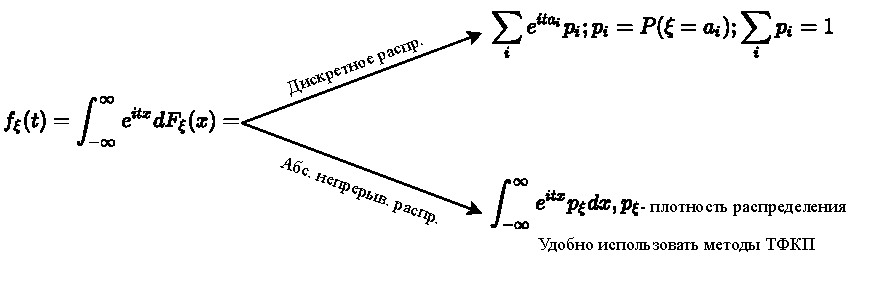
\includegraphics[scale=1.05]{./media/characteristic_function.pdf}}
\end{figure}
\begin{exmp}
	Вычислить характеристические функции:
	\begin{enumerate}
		\item[а)] Распределения Бернулли: $P(\xi = 1) = 1 - P(\xi = 0) = p$
		
		\textit{Решение:}
		\[ f_{\xi} (t) = e^{it 0} + p e^{it} = 1 + p e^{it} \]
		
		\item[б)] Распределение Пуассона: $P(\xi = i) = \frac{\lambda^i}{i!} e^{- \lambda}, i = 1, 2, \dots$
		
		\textit{Решение:}
		\[ f_{\xi} (t) = \sum_{k=0}^{\infty} e^{it k} \frac{\lambda^k}{k!} e^{-\lambda} = e^{-\lambda} \sum_{k=0}^{\infty} \frac{(\lambda e^{it})^k}{k!} \underset{\text{Ряд Тейлора}}{=} e^{\lambda e^{it}} e^{-\lambda} = e^{\lambda (e^{it} - 1)} \]
		
		\item[в)] Равномерное распределение $U(0, 1):$
		\[
		p_{\xi} (x) =
		\begin{cases}
		1, &x \in [0, 1] \\
		0, &x \notin [0, 1]
		\end{cases}
		\]
		
		\textit{Решение:}
		\[ f_{\xi} (t) = \int_{0}^{1} e^{it x} dx = \int_{0}^{1} (\cos (tx) + i \sin (tx)) dx = \frac{1}{t} \sin tx \bigg|_{0}^{1} + i \frac{1}{t} (- \cos (tx)) \bigg|_{0}^{1} = \]
		\[ = \frac{1}{t} ( \sin (t) + i ( - \cos (t) + 1 ) ) = \frac{1}{it} ( i \sin (t) + \cos (t) - 1 ) = \frac{1}{it} (e^{it} - 1) \]
		
		\item[г)] \hypertarget{normal_distribution}{Нормальное (стандартное) распределение (или распределение Гаусса)} $\mathcal{N}(0, 1):$
		\[ p_{\xi} (x) = \frac{1}{\sqrt{2 \pi}} e^{- \frac{x^2}{2}}, x \in \mathbb{R} \]
		
		\textit{Решение (удобно использовать ТФКП):}
		\[ f_{\xi} (t) = \int_{-\infty}^{\infty} e^{itx} \frac{1}{\sqrt{2 \pi}} e^{- \frac{x^2}{2}} dx = \int_{-\infty}^{\infty} \frac{1}{\sqrt{2 \pi}} e^{it x - \frac{x^2}{2}} dx = \int_{-\infty}^{\infty} \frac{1}{\sqrt{2 \pi}} e^{- \frac{(x - it)^2}{2}} e^{- \frac{t^2}{2}} dx = \]
		\[ = e^{- \frac{t^2}{2}} \int\limits_{-\infty - it}^{\infty - it} \frac{1}{\sqrt{2 \pi}} e^{- \frac{y^2}{2}} dy = \dots \]
		Интеграл по замкнутому контуру $= 0 +$ быстро убывает на $\infty \Rightarrow$
		\[ \int\limits_{-\infty - it}^{\infty - it} \frac{1}{\sqrt{2 \pi}} e^{- \frac{y^2}{2}} dy = \int_{-\infty}^{\infty} \frac{1}{\sqrt{2 \pi}} e^{-\frac{u^2}{2}} du = 1 \]
		\[  \dots = e^{- \frac{t^2}{2}} \]
		\begin{figure}[H]
			\center{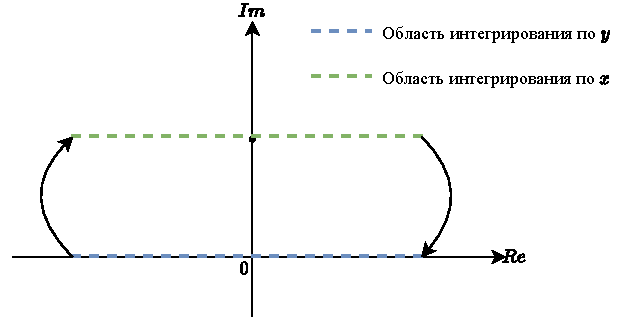
\includegraphics[scale=1]{./media/integration_area.pdf}}
		\end{figure}
	\end{enumerate}
\end{exmp}
\begin{center}
	\textbf{Свойства характеристических функций}
\end{center}
\begin{enumerate}
	\item $|f_{\xi} (t)| \le 1$
	\item $f_{\xi} (0) = 1$
	\item $f_{\xi} (-t) = \overline{f_{\xi} (t)}$ (см. 10-ый пункт)
	\item $f_{\alpha \xi + \beta} (t) = e^{it \beta} \cdot f_{\xi} (\alpha t)$
	\item $f_{\xi}$ - равномерно непрерывна на $\mathbb{R}$ (т.е. $\forall \epsilon > 0 \exists \delta > 0: \forall t_1, t_2: |t_1 - t_2| < \delta \Rightarrow |f_{\xi} (t_1) - f_{\xi} (t_2)| < \epsilon $)
	\item Если $\xi, \eta$ - независимые случайные величины, то $f_{\xi + \eta} (t) = f_{\xi} (t) \cdot f_{\eta} (t)$. Обратное утверждение неверное.
	\item Пусть $E |\xi|^k < \infty$. Тогда $f_\xi$ - $k$ раз дифференцируема, причём $f_{\xi}^{(k)} (0) = i^k E \xi^k (E\xi^k = j^{-k} f_{\xi}^{(k)} (0))$
	\item Формула Тейлора. Если $\exists E |\xi|^k < \infty$, то
	\[ f_{\xi} (t) = f_{\xi} (0) + \sum_{j = 1}^{n} \frac{t^j f_{\xi}^{(j)} (0)}{j!} + \bar{\bar o} (|t|^k) = 1 + \sum_{j=1}^{k} \frac{i^j t^j}{j!} E \xi^j + \bar{\bar o} (|t|^k) \]
	\item Формула обращения:
	\[ F_{\xi} (b) - F_{\xi} (a) = \frac{1}{2 \pi} \lim_{T \to \infty} \int_{-T}^{T} \frac{e^{-ita} - e^{-i+b}}{it} f_{\xi} (t) dt \]
	\item[9'.] $\xi$ - абсолютно непрерывная, $p_{\xi}$ - плотность распределения.
	\[ p_{\xi} (x) = \frac{1}{2 \pi} \int_{-\infty}^{\infty} e^{-it x} f_{\xi} (t) dt \]
	\item[9''.] $f_{\xi}$ - полностью определяет распределение $F_{\xi}$.
	\item Эрмитовость.
	
	$f_{\xi} (t) = \overline{f(-t)}$ (комплексно сопряжённая - очевидно).
	
	\item $\xi$ - симметрична относительно нуля $\eq f_{\xi} (t)$ - вещественная.
\end{enumerate}
\begin{proof}
	Докажем приведённые свойства:
	\begin{enumerate}
		\item $|f_{\xi} (t)| = | E e^{it \xi} | \le E |e^{it \xi}| = E1 = 1$
		\item $f_{\xi} (0) = E e^{i 0 \xi} = E1 = 1$
		\item $f_{\xi} (-t) = E \cos (-t \xi) + i E \sin (-t \xi) = E \cos (t \xi) - i E \sin (t \xi) = \overline{f_{\xi} (t)}$
		\item $f_{\alpha \xi + \beta} (t) = E e^{(\alpha \xi + \beta) it} = e^{it \beta} E e^{i (\alpha t) \xi} e^{it \beta} f_{\xi} (\alpha t)$
		\item $|f_{\xi} (t + h) - f_{\xi} (t)| = | E ( e^{i ( t + h ) \xi} - e^{it \xi} ) | = | E e^{it \xi} ( e^{i h \xi} - 1 ) | \le E | e^{it \xi} | | e^{ih \xi} - 1 | = E | e^{ih \xi} - 1 | \underset{h \to 0}{\to} = 0$,
		так как $| e^{ih \xi} - 1 | \le 2$ и $| e^{it \xi} | = 1$, а также имеется поточечная сходимость. Согласно теореме Лебега этого достаточно для сходимости.
		\item $f_{\xi + \eta} (t) = E e^{it (\xi + \eta)} = E e^{it \xi} e^{it \eta} = E e^{it \xi} E e^{it \eta} = f_{\xi} (t) f_{\eta} (t)$, поскольку из независимости $\xi$ и $\eta$ следует независимость $e^{it \xi}$ и $e^{it \eta}$.
		
		\item 
		\[ f_{\xi} (t) = E e^{it \xi} = \int_{-\infty}^{\infty} e^{it x} d F_{\xi} (x) \]
		Дифф-е под интегралом (идея):
		\[ f_{\xi}' = \int_{-\infty}^{\infty} i x e^{it x} d F_{\xi} (x) = i \int_{-\infty}^{\infty} x e^{it x} d F_{\xi} (x) \]
		\[ f_{\xi}'' = \int_{-\infty}^{\infty} (ix)^2 e^{it x} d F_{\xi} (x) = i^2 \int_{-\infty}^{\infty} x^2 e^{it x} d F_{\xi} (x) \]
		\[ f_{\xi}^{(k)} = \left( \int_{-\infty}^{\infty} (ix)^{k-1} e^{itx} d F_{\xi} (x) \right)' = \int_{-\infty}^{\infty} (ix)^k e^{itx} d F_{\xi} (x) = i^k \int_{-\infty}^{\infty} x^k e^{it x} d F_{\xi} (x) \]
		\[ \Rightarrow f_{\xi}^{(k)} (0) = i^k E \xi^k \]
		\item Док-во следует из св-в 7 и 1.
		
	\end{enumerate}
\end{proof}
\begin{definition}\label{sp_property}
	$\xi_n \Rightarrow \xi$ (последовательность $\xi_n$ сходится по распределению к величине $\xi$), если
	\[ F_{\xi_n} (x) \underset{n \to \infty}{\to} F(x), \forall x : F(x) - \text{ непрерывна в } (\cdot) x \]
	Тогда следующие утверждения равносильны:
	\begin{enumerate}
		\item $\xi_n \Rightarrow \xi$
		\item $f_{\xi_n} (t) \to f_{\xi} (t)$ для $\forall t \in \mathbb{R}$
	\end{enumerate}
\end{definition}
\begin{theorem}[Бохнера-Хинчина]
	$f$ - непрерывная, $f: \mathbb{C} \to \mathbb{R}; f(0) = 1$.
	
	Тогда $f$ - характеристическая функция некоторого распределения $\eq$ $f$ - неотрицательно определённая, т.е. $\forall u_1, \dots, u_m \in \mathbb{R}; z_1, \dots, z_m \in \mathbb{C}$
	\[ \sum_{ij = 1}^{m} f ( u_i - u_j ) z_i \bar z_j \ge 0 \]
\end{theorem}
\begin{remark}
	На практике применения теоремы Бохнера-Хинчина затруднительно. Обычно для проверки, что функция является характеристической использует 9. Нарушение свойств 1, 2, 5, 10 (одного из) $\Rightarrow$ функция не является характеристической.
\end{remark}
\begin{exmp}\label{second_exmple}
	Пусть $x_1, x_2, \dots$ - независимые и одинаково распределённые случайные величины.
	\[ p_{x_1} (x) = ( 1 - |x| ) 1_{\eta x \in [-1, 1]} \]
	
	\begin{center}
		\fbox{%
			\parbox[t][4.5cm]{13cm}{%
				Пусть $A \subseteq X$ - выбранное подмножество произвольного множества $X$. Функция $1_{A}: X \to \{0, 1\}$, определенная следующим образом:
				\[
				1_{A} (x) =
				\begin{cases}
				1, &x \in A, \\
				0, &x \notin A,
				\end{cases}
				\]
				называется индикатором множества $A$.
				
				Альтернативными обозначениями \textbf{индикатора множества} $A$ являются $\chi_A$ или $I_{A}$.
		}}\qquad
	\end{center}
	
	В дальнейшей для обозначения индикатора множества $A$ будем использовать $\chi_A$.
	
	\begin{enumerate}
		\item[а)] Найти характеристическую функцию $x_1$.
		
		\textit{Решение:}
		
		\[ f_{x_1} (t) = \int_{-1}^{1} e^{it x} (1 - |x|) dx = \int_{-1}^{1} ( \cos (tx) + i \sin (tx) ) (1 - |x|) dx = \]
		\[ = \int_{-1}^{1} \cos (tx) (1 - |x|) dx = 2 \int_{-1}^{1} \cos (tx) (1 - x) dx = \frac{2 \sin (tx)}{t} \bigg|_{0}^{1} - 2 \int_{0}^{1} x \cos (tx) dx = \dots \]
		
		\[
		\int_{0}^{1} x \cos (tx) dx = \int_{0}^{t} \frac{u}{t} \cos (u) \frac{du}{t} = \frac{1}{t^2} \int_{0}^{t} u \cos u du = \frac{1}{t^2} \int_{0}^{t} u d \sin u =
		\]
		\[
		= \frac{1}{t^2} \left( u \sin u \bigg|_{0}^{t} - \int_{0}^{t} \sin u du \right) = \frac{1}{t^2} (t \sin t + \cos t - 1)
		\]
		
		\[ \dots = \frac{2 \sin t}{t} - \frac{2 \sin t}{t} - \frac{2 \cos t}{t^2} + \frac{2}{t^2} = \frac{2 (1 - \cos t)}{t^2} \left[ = \frac{4 \sin^2 \frac{t}{2}}{t^2} \right] \]
		
		\item[б)] С использованием (а) найти $Ex_1, Dx_1$
		
		\textit{Решение:}
		
		\[ Ex_1 = \frac{f_{x_1}' (0)}{i} = 0; ~~~ Ex_1^2 = \frac{f_{x_1}'' (0)}{i^2} = - f_{x_1}'' (0) = \frac{1}{6}; ~~~ Dx_1 = \frac{1}{6} \]
		\[ f_{x_1}' (t) = \frac{2 t \sin t - 4 (1 - \cos t)}{t^3} = \frac{( 2t ( t + \bar{\bar o} (t^2) - 4\left( \frac{t^2}{2} + \bar{\bar o} (t^3) \right) ) )}{t^3} = \frac{2t^2 + \bar{\bar o} (t^3) - 2t^2 + \bar{\bar o} (t^3)}{t^3} \underset{t \to 0}{\to} 0 \]
		\[ \sin x = x - \frac{x^3}{3!} + \frac{x^5}{5!} + \bar{\bar o} (x^5); ~~~ \cos x = 1 - \frac{x^2}{2} + \frac{x^4}{4!} + \bar{\bar o} (x^4) \]
		\[ f_{x_1}'' (t) = 2 \left( \frac{t^2 \cos t - 4 t \sin t + 6 (1 - \cos t)}{t^4} \right) = \]
		\[ = 2 \left( \frac{\left( t^2 - \frac{t^2}{2} + \bar{\bar o} (t) \right) - \left( 4t^2 + \frac{4t^2}{6} + \bar{\bar o} (t^4) \right) + \left( 3t^2 - \frac{t^4}{4} + \bar{\bar o} (t^4) \right)}{t^4} \right) = \]
		\[ = \frac{- \frac{1}{6} t^4 + \bar{\bar o} (t^4)}{t^4} \to - \frac{1}{6} \]
		\textbf{(!)} В данном случае, проще было найти мат. ожидание через интеграл.
		\item[в)] Найти характеристическую функцию разности $x_1 - x_2; x_1, x_2$ - независимые величины с плотностью $p_{x_1}$.
		
		\textit{Решение:}
		
		Используем св-ва 4 и 6:
		\[ f_{- x_2} (t) = f_{x_1} (-t) = f_{x_1} (t) \]
		\[ f_{x_1-x_2} (t) = f_{x_1} (t) f_{x_1} (-t) = |f_{x_1} (t)|^2 \underset{\text{т.к. веществ.}}{=} \frac{4 (1 - \cos t)^2}{t^4} = \frac{16 \sin^4 \frac{t}{2}}{t^4} \]
		
		\item[г)] Найти характеристическую функцию $Y = 6x_1 + 2x_2 - 3$.
		
		\textit{Решение (аналогично В):}
		
		\[ f_{Y} (t) = f_{6 x_1} (t) f_{2x_2 + 3} (t) = e^{i \cdot 3 \cdot t} f_{x_1} (6t) f_{x_2} (2t) = \]
		\[ = e^{i \cdot 3t} \frac{4 (1 - \cos 6t) (1 - \cos 2t)}{36 t^2 \cdot 4 t^2} = \frac{e^{i \cdot 3t} (1 - \cos (6t)) (1 - \cos 2t)}{36t^4} \]
		
		\item[д)] Найти характеристическую функцию $z_n = \frac{1}{n} \sum\limits_{i = 1}^{n} x_i$.
		
		\textit{Решение:}
		
		Используем свойства 4 и 6 (рекурсивно):
		
		\[ f_{z_n} (t) = \prod_{i=1}^{n} f_{\frac{x_i}{n}} (t) = \left( f_{x_1} \left( \frac{t}{n} \right) \right)^n = \frac{2^n \left( 1 - \cos \frac{t}{n} \right)^n}{t^{2n}} \]
		\textbf{(!)} Дополнительно проследим поведение $f_{z_n}$ при $n \to \infty$.
		\[ f_{z_n} (t) = \frac{2^n \left( \frac{t^2}{2n^2} + \bar{\bar o} \left( \frac{1}{n^3} \right) \right)^n}{\left( \frac{t}{n} \right)^{2n}} = \left( \frac{2t^2}{2n^2} : \left( \frac{t}{n} \right)^2 + \bar{\bar o} \left( \frac{1}{n} \right) \right)^n = \left( 1 + \bar{\bar o} \left( \frac{1}{n} \right) \right)^n \underset{n \to \infty}{\to} 1, \forall t \]
		\textbf{(!)} Изучим $f_{z} (t) = 1, \forall t \eq p(z = 0) = 1$
		Согласно св-ву \ref{sp_property} $z_n \Rightarrow z$ (сходится по распределению).
		\[ p (z_n < x) \underset{n \to \infty}{\to} p(z < x), x \ne 0 (\text{ в точке } x = 0 ~ F_{z} \text{ разрывна, т.е.} ) \]
		\[
		\begin{cases}
		p(z_n < x) \to 0, &x < 0 \\
		p(z_n < x) \to 1, &x > 0
		\end{cases}
		\Rightarrow
		p(|z_n| < \delta) = \underset{n \to \infty, \to 1}{F_{z_n} (\delta)} - \underset{n \to \infty, \to 0}{F_{z_n} (- \delta_{+})} \underset{n \to \infty}{\to} 1, \delta > 0 \Rightarrow
		\]
		\[ \Rightarrow p( |z_n| \ge \delta ) \underset{n \to \infty}{\to} 0, \forall \delta > 0 \text{ ЗБЧ.} \]
		\textbf{(!)} В общем случае, $x_1, \dots, x_n$ - нез. одинак. распределённые, $Ex_1 = a, z_n = \frac{1}{n} \sum\limits_{i=1}^{n} x_i$.
		\[ \log (f_{z_n} (t)) = \log \left( f_{x_1} \left( \frac{t}{n} \right) \right)^n = n \log f_{x_1} \left( \frac{t}{n} \right) \underset{\text{ф-л Тейлора}}{=} n \cdot \left( i a \left( \frac{t}{n} \right) + \bar{\bar o} \left( \frac{1}{n} \right) \right) = i at + \bar{\bar o} (1) \underset{n \to \infty}{\to} i at \]
		\[ g(n) = \log f_{x_1} (u); ~~~ g' (u) = \frac{f_{x_1}' (u)}{f_{x_1} (u)} \bigg|_{u = 0} = \frac{f_{x_1}'(0)}{f_{x_1} (0)} = \frac{ia}{1} \]
		т.о. $f_{z_n} (t) \underset{n \to \infty}{\to} e^{iat}$ - характеристическая функция с.в. $z: p(z = a) = 1$. тогда $z_n \Rightarrow z$, откуда следует сходимость по вероятности.
		\item[е)] Найти характеристическую функцию величины $T_n = n^{-\frac{1}{2}} \sum\limits_{i=1}^{n} x_i$.
		
		\textit{Решение (аналогично Д):}
		
		\[ f_{T_n} (t) = \prod_{i=1}^{n} f_{\frac{x_i}{\sqrt{n}}} (t) = \left( f_{x_1} \left(\frac{t}{\sqrt{n}}\right)^n = \frac{2^n (1 - \cos \left( \frac{t}{\sqrt{n}} \right))^n}{t^{2n}/n^n} \right) \]
		\textbf{(!)} Проследим поведение $f_{T_n}$ при $n \to \infty$
		\[ f_{T_n} (t) = \left( \frac{2 (1 - \cos \left( \frac{t}{\sqrt{n}} \right))}{t^2 / n} \right)^n = \left( \frac{2 \left( \frac{t^2}{2n} - \frac{t^4}{24n^2} + \bar{\bar o} (t^4) \right)}{t^2 / n} \right)^n = \left( 1 - \left( \frac{t^2}{12n} + \bar{\bar o} \left( \frac{1}{n} \right) \right) \right)^n = \]
		\[ = \left( \underset{\underset{n \to \infty}{\to} e}{\left( 1 - \left( \frac{t^2}{12n} + \bar{\bar o} \left(\frac{1}{n}\right) \right) \right)^{-\frac{12n}{t^2}}} \right)^{- \frac{t^2}{12}} \underset{n \to \infty}{\to} e^{- \frac{t^2}{12}} \text{ замечательные предел} \]
		\textbf{(!)} Идентифицируем распределение $T: f_{T} (t) = e^{-\frac{t^2}{12}}$
		\[ f_{T} (t) = f_{\xi} \left( \frac{t}{\sqrt{6}} \right), \text{ где } \xi \sim N(0, 1) \text{ см. пред. задачу (г) } f_{\xi} (u) = e^{- \frac{u^2}{2}} \]
		Таким образом $T \sim \frac{\xi}{\sqrt{6}}$, т.е. $T \sim N \left( 0, \frac{1}{6} \right)$
		\textbf{(!)} Используем св-во \ref{sp_property} $T_n \underset{n \to \infty}{\Rightarrow} T$, т.е.
		\[ P(T_n < x) \underset{n \to \infty}{\to} P(T < x), \forall x \in \mathbb{R} (\text{т.к. } F_T \text{ - непрерывная}) \]
		Перепишем
		\[ P(\sqrt{6} T_n < x) \to P(\xi < x) = \Phi (x) \text{ Центральная предельная теорема.} \]
		\textbf{(!)} В общем случае при $a = Ex_1 = 0, \sigma^2 = Dx_1 < \infty; T_n = \frac{1}{\sqrt{n}} \sum\limits_{i=1}^{n} x_i$.
		\[ \log f_{T_n} (t) = n \log f_{x_1} \left( \frac{t}{\sqrt{n}} \right) = \dots \]
		По формуле Тейлора:
		\[
		g(u) = \log f_{x_1} (u); g(0) = 0; g'(u) = \frac{f_{x_1}'(u)}{f(u)} \bigg|_{u=0} = \frac{f_{x_1}' (0)}{1} = i Ex_1 =
		\]
		\[
		= \frac{f_{x_1}'' (u) f_{x_1} (u) - f_{x_1}' (u)^2}{f(u)^2} \bigg|_{u=0} = \frac{i^2 E x_1^2 \cdot 1 - (i Ex_1)^2}{1} = - \sigma^2
		\]
		\[ \dots = n \left( ia \frac{t}{\sqrt{n}} - \frac{\sigma^2}{2} \frac{t^2}{n} + \bar{\bar o} \left( \frac{1}{n} \right) \right) \overset{a=0}{\underset{n \to \infty}{\to}} - \frac{\sigma^2 t^2}{2}; f_{T_n} (t) \underset{n \to \infty}{\to} e^{- \frac{t^2 \sigma^2}{2}} \]
		Тогда
		\[ T_n \underset{n \to \infty}{\Rightarrow} T \sim N (0, \sigma^2) \text{ или } \frac{T_n}{\sigma} \underset{n \to \infty}{\Rightarrow} N(0, 1) \text{, т.е.} \]
		\[ p \left( \frac{\sum\limits_{i=1}^{n} x_i}{\sqrt{n} \sigma} < x \right) \underset{n \to \infty}{\to} \Phi (x), \forall x \in \mathbb{R} \]
		Центральная предельная теорема Леви.
	\end{enumerate}
\end{exmp}

\begin{exmp}
	Является ли характеристической функция $f(t) = (1 - |t|) \chi_{ \{ t \in [-1, 1] \} } $
	
	\textit{Решение:}
	
	Свойства $1,2,5,10$ выполнены, но это не доказывает, что $f(t)$ - характеристическая.
	
	Воспользуемся формулой обращения для плотности
	\[
	p(t) = \frac{1}{2 \pi} \int_{-1}^{1} e^{-itx} (1 - |x|) dx = \frac{1}{2 \pi} \left( \underset{=\frac{2(1 - \cos x)}{x^2}}{\int_{-1}^{1} \cos (tx) (1 - |t|) dt} - \underset{=0}{i \int_{-1}^{1} \sin (tx) (1 - |t|) dt} \right) =
	\]
	\[ = \frac{1 - \cos x}{\pi x^2}, x \in \mathbb{R} ~~~ \left[ \int_{-\infty}^{\infty} p(t) dt = 1 \right] - \text{ плотность распределения.} \]
	Значит, $f(t)$ - характеристическая функция.
\end{exmp}
\begin{exmp}
	В задаче \ref{second_exmple} вычислить при $n = 1000$ (приближённо).
	\[ p \left( -30 \le \sum\limits_{i=1}^{n} x_i \le 30 \right) - ? \]
	
	\textit{Решение:}
	
	\[
	p \left( -30 \le \sum\limits_{i=1}^{1000} x_i \le 30 \right) = p \left( - \frac{30 \sqrt{6}}{10 \sqrt{10}} \le \frac{\sqrt{6} \sum\limits_{i=1}^{1000} x_i}{10 \sqrt{10}} \le \frac{30 \sqrt{6}}{10 \sqrt{10}} \right) =
	\]
	\[
	= p \left( - \frac{3 \sqrt{6}}{\sqrt{10}} \le T_n \sqrt{6} \le \frac{3 \sqrt{6}}{\sqrt{10}} \right) \approx \Phi \left( \frac{3 \sqrt{6}}{\sqrt{10}} \right) - \Phi \left( - \frac{3 \sqrt{6}}{\sqrt{10}} \right) = 2 \Phi \left( \frac{3 \sqrt{6}}{\sqrt{10}} - 1  \right) \approx 0.98
	\]
\end{exmp}

\section{Цепи Маркова}

\noindent Пусть $\xi_1, \dots, \xi_n, \dots$ - случайная последовательность (последовательность случайных величин).
\begin{definition}[Конечномерное распределение (КМР)]
	Распределение последовательности определяют конечномерные распределения
	\[ \mathcal{P}_{\xi_1, \dots, \xi_k} (A_1 \times \dots \times A_k) = p(\xi_1 \in A_1, \dots, \xi_k \in A_k), k \in \mathbb{N} \]
\end{definition}

\noindent\textbf{Условие согласования:}
\[ p(\xi_1 \in A_1, \dots, \xi_{k-1} \in A_{k-1}) = \mathcal{P}_{(\xi_1, \dots, \xi_k)} (A_1 \times \dots A_{k-1} \times \mathbb{R}) \]
\noindent\textbf{Марковское свойства:}
\[ p(\xi_{k+1} \in A_{k+1} | \xi_1 = x_1, \dots, \xi_k = x_k) = p (\xi_{k+1} \in A_{k+1} | \xi_k = x_k),\]
\[\forall x_1, \dots, x_k \in \mathbb{R} (\text{почти наверное}), \forall A_{k+1} \in \mathcal{B}_1, k \in \mathbb{N} \]
\begin{definition}[Цепь Маркова]
	Цепь Маркова - последовательность случайных величин, удовлетворяющих Марковскому свойству.
	\[ \forall i ~ \exists E_i: p(\xi_i \in E_i) = 1 \& E_i - \text{ не более, чем счётное } \Rightarrow E = \bigcup_{i \in \mathbb{N}} E_i - \text{ не более, чем счётное} \]
	$E$ - \textit{множество состояний} цепи Маркова.
\end{definition}
\subsection{КМР цепи Маркова}

\[ p(\xi_1 = i_1, \dots, \xi_k = i_k) = p(\xi_k = i_k | \xi_{k-1} = i_{k-1}) \cdot p(\xi_{k-1} = i_{k-1} | \xi_{k-2} = i_{k-2}) \cdot ... \cdot p(\xi_2 = i_2 | \xi_1 = i_1) p(\xi_1 = i_1) \]

\noindent\textit{Обозначения:}
\[ q_j = p(\xi_1 = j), j \in E - \text{ начальное распределение} \]
\[ p_{ij} (k) = p(\xi_{k+1} = j | \xi_k = i), i,j \in E, k \in \mathbb{N} - \text{ вероятности перехода} \]

\subsection{Однородные цепи Маркова}
\[ p_{ij} (k) = p_{ij}, \forall k \in \mathbb{N} \text{ (вероятности перехода не зависят от } k) \]

\noindent\textbf{(!)} Для задания распределения однородной ЦМ достаточно $\{ q_j \}, j \in E$ - начальное распределение вероятностей, $\sum\limits_{j \in E} q_j = 1$.

$\mathbb{P} = || p_{ij} ||_{i,j \in E}$ - матрица (возможно бесконечная) вероятностей перехода.

\noindent\textbf{Вероятность перехода} за $s$ шагов (однородная ЦМ):
\[ p_{ij}^{(s)} = p(\xi_{k+s} = i | \xi_k = j) \]

\noindent\textbf{Уравнение} Маркова (формула полной вероятности)
\[ p_{i,j}^{r+s} = \sum_{k \in E} p_{ik}^{(r)} p_{kj}^{(s)}, \forall i,j \in E; r,s \in \mathbb{N} \]
Вывод: в однородной цепи Маркова
\[ p^{(s)} = || p_{ij}^{(s)} || = \underbrace{P \times ... \times P}_{*} = p^s, * - s \text{ раз умножение матрицы \linebreak по правилам матричного умножения} \]

Структуру однородной цепи Маркова характеризует матрица вероятностей перехода (МВП) или граф.
\begin{enumerate}
	\item (Случайное блуждание) Заданы начальные распределения вероятностей:
	\[
	q_i =
	\begin{cases}
		1, &i = 0 \\
		0, &i \ne 0
	\end{cases}
	~~~~~~
	E = \mathbb{Z} \text{ и МВП }
	p_{ij} =
	\begin{cases}
		p, &j = i + 1 \\
		1 - p, &j = i - 1 \\
		0, j \notin \{i-1,i+1\}\}
	\end{cases}
	\]
\end{enumerate}

\begin{exmp}\label{cm-ex_1}
	Построить граф однородной цепи Маркова, найти вероятности перехода за $k$ шагов $k \in \mathbb{N}$.
	\[
	P = 
	\begin{pmatrix}
		\ldots       & \ddots & p   & 0 & \hdotsfor{3} \\
		\ldots       & 1-p    & 0   & p & 0 & \hdotsfor{2} \\
		\ldots       & 0      & 1-p & 0 & p & 0 & \ldots \\
		\hdotsfor{2} & 0      & 1-p & 0 & p & 0 \\
		\hdotsfor{3} & 0      & 1-p & 0 & p \\
		\hdotsfor{4} & 0      & 1-p & \ddots
	\end{pmatrix}
	\]
\end{exmp}
\begin{center}
	\underline{Граф}
\end{center}
\begin{figure}[h]
	\center{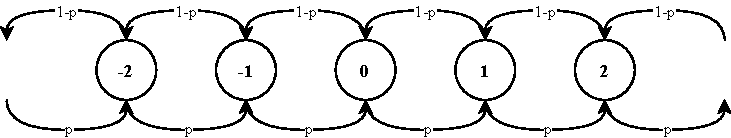
\includegraphics[scale=1.1]{./media/cm-graph_1.pdf}}
\end{figure}
Вероятность перехода за $k$ шагов (сх. Бернулли, $\xi_{k+1} =$ число успехов в $k$ испытаниях - число неудач).
\[
p_{ij}^{(k)} =
\begin{cases}
	C_k^{\frac{k+j-i}{2}}p^{\frac{k+j-i}{2}} (1-p)^{\frac{k-j+i}{2}}; k+j - \text{ чётное}; i-j \in [-k, k] \\
	0 - \text{ в остальных случаях}
\end{cases}
\]

\begin{exmp}\label{cm-ex_2}
	Задан граф однородной цепи Маркова.
	\begin{figure}[h]
		\center{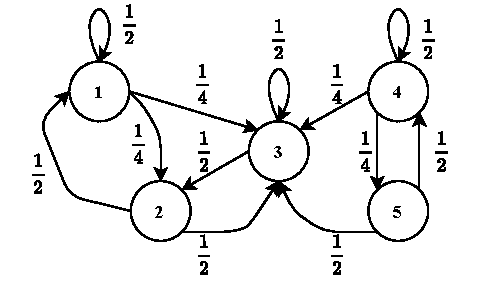
\includegraphics[scale=1.15]{./media/cm-graph_2.pdf}}
	\end{figure}
	\begin{enumerate}
		\item[а)] Восстановить МВП;
		\item[б)] Найти МВП за 2 шага.
	\end{enumerate}
	\textit{Решение:}
	\[
	\text{а)} ~~~
	p =
	\begin{pmatrix}
		1/2 & 1/4 & 1/4 & 0 & 0 \\
		1/2 & 0 & 1/2 & 0 & 0 \\
		0 & 1/2 & 1/2 & 0 & 0 \\
		0 & 0 & 1/4 & 1/2 & 1/4 \\
		0 & 0 & 1/2 & 1/2 & 0
	\end{pmatrix}
	~~~~~~
	p^2 =
	\begin{pmatrix}
		3/8 & 1/4 & 3/8 & 0 & 0 \\
		1/4 & 3/8 & 3/8 & 0 & 0 \\
		1/4 & 1/4 & 1/2 & 0 & 0 \\
		0 & 1/8 & 3/8 & 3/8 & 1/8 \\
		0 & 1/4 & 3/8 & 1/4 & 1/8
	\end{pmatrix}
	\]
\end{exmp}
\begin{remark}
	сумма элементов матрицы по строке равна 1.
\end{remark}
\noindent\textbf{МВП} - стохастическая матрица.

\subsection{Изучение структуры однородной цепи Маркова}

\begin{enumerate}
	\item $i \to j$ ($j$ достижимо из $i$), если $\exists s: p_{ij}^{(s)}>0$
	\item Если $i \to j$ и $j \to i$, то состояния $i,j$ сообщаются
	\item Если $\exists j: i \to j$, но $j \not\to i$, то $j$ - несущественное; в противном случае $j$ - существенное.
\end{enumerate}

\textbf{Утв. 1.} Все существенные состояния однородной ЦМ можно разделить на \textit{классы сообщающихся} состояний, которые не пересекаются, и любые два состояния внутри класса сообщаются, а состояния из разных классов недостижимы друг для друга.

\noindent\textbf{(!)} Однородная ЦМ, состоящая из одного класса сообщающихся состояний - \textit{неприводима} (НЦМ).

Период НЦМ: $T = \text{НОД}(s: p_{ii}^{(s)} > 0)$

\textbf{Утв. 2.}
\begin{enumerate}
	\item Период НЦМ не зависит от выбора $i$.
	\item Все состояния НЦМ можно разделить на $T$ непересекающихся классов, так что на каждом шаге с вероятностью 1 происходит переход из $\forall$ состояния класса $r$ в какое-то состояние класса $r+1, r \in \{1, \dots, T-1\}$, и из $\forall$ состояния класса $T$ - в какое-то состояние класса 1.
\end{enumerate}
\begin{remark}
	Классы из утв. 2 (2) - \textit{циклические подклассы}.
\end{remark}

\begin{exmp}
	Классифицировать состояния ЦМ из задачи \ref{cm-ex_1}.
	
	Для решения удобнее использовать граф.
	\begin{enumerate}
		\item[а)] Очевидно, что все состояния сообщаются $\Rightarrow$ ОЦМ неприводима.
		\item[б)] $T=2$, т.к. $p_{ii}^{(s)} = 0$, если $s$ - нечётное (см. задачу \ref{cm-ex_1}).
		
		Циклические подклассы: $C_1 = \{ i: i - \text{ чётное} \}, C_2 = \{ i: i - \text{ нечётное} \}$.
	\end{enumerate}
\end{exmp}
\begin{exmp}
	Классифицировать состояния ЦМ из задачи \ref{cm-ex_2}.
	
	Для решения используем граф (состояния неважны).
	\begin{enumerate}
		\item[а)] Отметим $4 \to 3$, но $3 \not\to 4$ И $5 \to 3$, но $3 \not\to 5 \Rightarrow$ вершины $4$ и $5$ - несущественны. Остальные состояния сообщаются: $1 \eq 2, 2 \eq 3, 1 \eq 3$.
		
		ОЦМ, состоящая из вершин $(1, 2, 3)$ - неприводима.
		\item[б)] $T=1$, т.к. $p_{11} > 0$ (петля). ОЦМ непериодическая.
		
		\textbf{(!)} Если удалить несуществующие состояния и переставить состояния должным образом, то МВП может быть сделана блочно-диагональной (каждый блок соответствует НЦМ).
	\end{enumerate}
	\begin{figure}[h]
		\center{\includegraphics[scale=1.15]{./media/cm_matrix.pdf}}
	\end{figure}
\end{exmp}

\subsection{Возвратность, эргодичность, финальные вероятности}

\noindent Вероятность возвращения на $s$-м шаге впервые
\[ f_{ii}^{(s)} = p (\xi_{k + s} = i, \xi_{k+s-1} \ne i, \dots, \xi_{k+1} \ne i | \xi_k = i) \]
Вероятность возвращения в состояние $i$:
\[ f_i = \sum_{s=1}^{\infty} f_{ii}^{(s)} \le 1 \]
\textbf{(!)} Состояние $i$ \textit{возвратное}, если вероятность возвращения $f_i = 1$.

Состояние $i$ \textit{эргодичное}, если среднее время возвращения конечно
\[ E \tau_i = \sum_{s=1}^{\infty} s f_{ii}^{(s)} < \infty, \]
где $\tau_i$ - время 1-ого возвращения в состояние $i$.

\textbf{Утв. 3.} В НЦМ все состояние однотипны (если одно возвратно, то все возвратны; если одно эргодическое, то все эргодические).

\textbf{Утв. 4.} (Критерий возвратности).
\begin{enumerate}
	\item Несущественные состояния невозвратны
	\item Состояние $i$ возвратно (т.е. $f_i=1$) $\eq \sum\limits_{s=1}^{\infty} p_{ii}^{(s)} = \infty$
	\item Состояние $i$ возвратно, но не эргодическое $\eq \sum\limits_{s=1}^{\infty} p_{ii}^{(s)} = \infty ~ \& ~ \lim\limits_{s \to \infty} p_{ii}^{(s)} = 0$
	\item Состояние эргодическое $\eq \sum\limits_{s=1}^{\infty} p_{ii}^{(s)} = \infty ~ \&$ не выполнено $\lim\limits_{s \to \infty} p_{ii}^{(s)} = 0$
\end{enumerate}

\textbf{Утв. 5.} (Эргодическая теорема)

\noindent В неприводимой непериодической эргодической (т.е. состояния эргодические) цепи Маркова
\[ \exists p_{j}^{*} = \lim_{m \to \infty} p_{ij}^{(m)} \]
независящие от $i$ и удовлетворяющих системе уравнений
\[
(*) =
\begin{cases}
	p_{j}^{*} = \sum\limits_{i \in E} p_{i}^{*} p_{ij}, j \in E \\
	\sum\limits_{j \in E} p_{j}^{*} = 1
\end{cases}
\]
Или в матричной форме:
\[
P^{*^T} (\mathbb{P} - I) = 0 ( (\mathbb{P}^T - I)p^* = 0 )
\]
\[
p^{*}=
\begin{pmatrix}
	p_1^* \\ p_2^* \\ \vdots \\ \vdots
\end{pmatrix}
\text{ с условием } \sum_j p_j^* = 1
\]

\textbf{(!)} Решение (*) единственно (в условиях утв. 5)

\textbf{(!)} При наличии нескольких классов сообщающихся состояний финальные вероятности (если классы эргодические) считаются в каждом из классов.

\textbf{(!)} При наличии периода можно рассмотреть ЦМ с шагом $T$.

\textbf{(!)} Финальные вероятности $p_i$ определяют среднее время нахождение НЦМ в соответствующем состоянии.

\textbf{(!)} Все состояния конечной НЦМ с периодом 1 - эргодическое.

\begin{exmp}
	Проверить свойства возвратности и эргодичности НЦМ из задача \ref{cm-ex_1}.
	\begin{enumerate}
		\item[а)] Возвратность. Согласно решению задачи \ref{cm-ex_1}:
		\[ p_{ii}^{(2k)} = C_{2k}^k p^{k} (1-p)^k, k \in \mathbb{N} ~~~~~~~~~ p_{ii}^{(2k-1)} = 0 \]
		Рассмотрим
		\begin{figure}[h]
			\center{\includegraphics[scale=1.15]{./media/cm-formula_1.pdf}}
		\end{figure}
		\[ \text{При } p = \frac{1}{2}: a_k = \frac{(2k)!}{(k!)^2} \left( \frac{1}{2} \right)^{2k} \left( = \frac{(2k-1)!!}{2k!!} = \frac{1 \cdot 3 \cdot 5}{2 \cdot 4 \cdot 6} = \prod_{i=1}^{k} \left( 1 - \frac{1}{i} \right) \right) \]
		По формуле Стирлинга:
		\[ a_k = \frac{ \sqrt{4 \pi k} \left( \frac{2k}{2} \right)^{2k} e^{-\theta_{2k}}}{(\sqrt{2 \pi})^2 \left( \frac{k}{e} \right)^{2k} e^{-\theta_k} \cdot 2^{2k}} = \frac{1}{\sqrt{\pi k}} e^{-\theta_{2n} + \theta_n} \sim \frac{1}{\sqrt{\pi k}} \]
		Поскольку $\int\limits_{1}^{\infty} \frac{1}{\sqrt{\pi x}} dx$ - расходится $\Rightarrow$ (интегральный признак) $\sum\limits_{k=1}^{\infty} a_k = \infty$.
		
		Ответ (а):
		\begin{itemize}
			\item При $p \ne \frac{1}{2}$ ЦМ невозврата (все состояния невозвратны)
			\item При $p = \frac{1}{2}$ ЦМ возвратна (все состояния возвратны)
		\end{itemize}
		\item[б)] Очевидно, что $\lim\limits_{k \to \infty} p_{ii}^{(2k)} = \lim\limits_{k \to \infty} \frac{1}{\sqrt{\pi k}} = 0 \Rightarrow$ ЦМ нулевая (не эргодическая) даже при $p = \frac{1}{2}$.
	\end{enumerate}
\end{exmp}

\begin{exmp}
	Найти финальные вероятности $p_1^*, p_2^*, p_3^*$ НЦМ, состоящей из состояний $1,2,3$ ЦМ, определённой в задаче \ref{cm-ex_1}.
	
	Эргодичность следует из последнего замечания перед примерами. Система уравнений:
	\[
	\begin{cases}
		p_1^* = p_1^* \cdot \frac{1}{2} + p_2^* \cdot \frac{1}{2} \\
		p_2 = p_1^* \frac{1}{4} + p_3^* \frac{1}{2} \\
		p_1 + p_2 + p_3 = 1
	\end{cases}	
	\]
	$\eq$ (уравнение $p_3 = p_1 \frac{1}{4} + p_2 \frac{1}{2} + p_3 \frac{1}{2}$ удалили, т.к. оно линейно зависимо с первыми двумя)
\end{exmp}
\textbf{(!)} Можно удалить любое из уравнений.
\[ p_i^* = \sum_j p_j p_{ji} \eq \begin{cases} p_1 = p_2 \\ p_3 = \frac{3}{2} p_1 \\ \frac{7}{2} p_1 = 1 \end{cases} \eq \begin{cases} p_1 = \frac{2}{7} \\ p_2 = \frac{2}{7} \\ p_3 = \frac{3}{7} \end{cases} \]

\textbf{(!)} В циклической НЦМ финальные вероятности не существуют. Рассмотрев НЦМ с матрицей перехода $\mathbb{P}^{(T)}$ можно получить финальные вероятности в каждом циклическом подклассе. Среднее время нахождения ЦМ в каждом состоянии равно отношению полученной финальной вероятности и число циклических подклассов ($=T$).

\textbf{(!)} Финальные вероятности можно получить приближённо по временам пребывания смоделированной ЦМ. В каждом из состояний на достаточно большом промежутке времени.

\newpage
\section{Дополнительные темы}

\subsection{$\sigma$-алгебра}\label{sigma}

Для обозначения $\sigma$-алгебры обычно используются каллиграфические заглавные буквы латинского алфавита, например $\mathcal{A, F, H}$.

\begin{definition}[Сигма-алгебра]
	Множество $\mathcal{F}$ называется $\sigma$-алгеброй для множества элементарных исходов $\Omega$, если:
	\begin{enumerate}
		\item $\emptyset, \Omega \in \mathcal{F}$;
		\item Если $A \in \mathcal{F}$, то $\bar A \in \mathcal{F}$;
		\item Если $A_1, A_2, \dots \in \mathcal{F}$, то любое событие, которое можно получить из $A_i$ с помощью любой логической операции \textit{в счетном количестве}, обязательно лежит в $\mathcal{F}$.
	\end{enumerate}
\end{definition}

\begin{definition}[Порождённая $\sigma$-алгебра]
	Говорим, что $\Event_{\xi}$ является $\sigma$-алгеброй, порождённой случайной величиной $\xi$.
\end{definition}

Приведем несколько примеров $\sigma$-алгебр, порожденных случайными величинами. Рассмотрим вероятностное пространство, в котором $\Omega = [0; 1], F = \Borel_{[0; 1]}$, а $P$ - мера Лебега, определенная на измеримых подмножествах отрезка $[0; 1]$.
\begin{enumerate}
	\item Если $\xi (\omega) \equiv c$, то $\Event_{\xi} = \{ \emptyset, \Omega \}$.
	\item Если $\xi (\omega) = \begin{cases} c_1, & \omega \in \left[ 0; \frac{1}{3} \right] \\ c_2, & \omega \in \left( \frac{1}{3}; 1 \right] \end{cases}$, где $c_1 \ne c_2$, то $\Event_{\xi} \{ \emptyset, \Omega, \left[0; \frac{1}{3}\right], \left(\frac{1}{3}; 1\right] \}$.
	\item Если $\xi(\omega) = \omega$, то $\Event_{\xi} = \Borel_{[0;1]}$.
\end{enumerate}

\begin{definition}
	Говорим, что $\xi_1, \xi_2, \dots, \xi_n$ - независимые случайные величины, если $\Event_{\xi_1}, \Event_{\xi_2}, \dots, \Event_{\xi_n}$ представляют собой независимые $\sigma$-алгебры.
\end{definition}

\begin{definition}[Борелевская сигма-алгебра]
	Борелевская сигма-алгебра — это минимальная сигма-алгебра, содержащая все открытые подмножества топологического пространства (впрочем, она содержит и все замкнутые). Обычно в качестве топологического пространства выступает множество вещественных чисел ($\mathbb{R}$). С борелевской сигма-алгеброй связано понятие борелевской функции.
\end{definition}

\begin{exmp}(Сигма-алгебра)
	Эксперимент заключается в однократном подбрасывании игрового кубика. Пространство элементарных исходов:
	\[ \Omega = \{ 1, 2, 3, 4, 5, 6 \} \]
	Имеется три наблюдателя эксперимента: Антон - знает что кубик бросали, но не видел что на нем выпало. Обозначим $\sigma$-алгебру Антона $\mathcal{F}$, Берта - внимательно наблюдала эксперимент, видела исход. Обозначим $\sigma$-алгебру Берты $\mathcal{H}$. Ваня - так же видел исход эксперимента, но он из южно-американского племени Пираху, где при счете различают только 1, 2 и “много”. $\sigma$-алгебра Вани - $\mathcal{V}$.
	
	Определим, из каких элементов состоит каждая $\sigma$-алгебра. Антон не видел исход эксперимента, но знал, что эксперимент был, таким образом он может ответить на вопрос: “Упал ли кубик?”, или по-другому: “Выпало ли какое-нибудь число?”. То есть Антон различает только два события: “кубик упал”, которому соответствует все пространство элементарных исходов, и любое иное невозможное утверждение как, например, что “кубик не упал”, которому соответствует пустое множество. Получаем, что $\mathcal{F} = \{ \emptyset, \Omega \}$.
	
	Берта видела исход эксперимента и различает все исходы, а значит, различает все возможные события, которые могут произойти в ходе эксперимента, их объединения, пересечения и прочие логические операции над ними ( мы предполагаем, что наши индивиды умеют делать логические выводы, на основе имеющейся информации). $\sigma$-алгебра Берты - булеан $\Omega$.
	
	Между делом посмотрим, как вычисляется булеан конечного множества. Вычислим мощность $\mathcal{H}$. Пусть событие $A_i$ - - на кубике выпало число очков, равное $i, i=1,2,\dots,6$. Элементы множества $\mathcal{H}$ - это все возможные события нашего эксперимента. Каждое событие можно представить в виде объединения всех $A_i$ или их дополнений $\bar A_i$.
	\[
	\begin{bmatrix}
	A_1 \\ \bar A_1
	\end{bmatrix}
	\cup
	\begin{bmatrix}
	A_2 \\ \bar A_2
	\end{bmatrix}
	\cup
	\begin{bmatrix}
	A_3 \\ \bar A_3
	\end{bmatrix}
	\cup
	\begin{bmatrix}
	A_4 \\ \bar A_4
	\end{bmatrix}
	\cup
	\begin{bmatrix}
	A_5 \\ \bar A_5
	\end{bmatrix}
	\cup
	\begin{bmatrix}
	A_6 \\ \bar A_6
	\end{bmatrix}
	\]
	То есть $A_i$ означает, что мы “включаем” $i$-ый исход, а $\bar A_i$ - “исключаем” $i$-ый исход.
	
	С помощью простых комбинаторных методов считаем все возможные комбинации таких событий, получаем:
	\[ card\mathcal{H}=2^6=64 \]
	То есть в $\sigma$-алгебре Берты 64 элемента. В общем случае мощность булеана конечного множества $A$, в котором $n$ элементов, вычисляется по формуле:
	\[ card \mathcal{P} (A) = 2^n \]
	
	В ситуации с Антоном и Бертой все достаточно просто, у Вани же дела обстоят немного интереснее. Рассмотрим некоторые примеры событий и выясним, лежат ли они в $\sigma$-алгебре Вани или нет. “Выпало 1” $= \{ 1 \} \in \mathcal{V}$, так как Ваня знает что такое 1. “Выпало 5” $- \{ 5 \} \notin \mathcal{V}$, так как все, что больше 2 Ваня считает за “много”, следовательно 5 к примеру от 3 или 6 он не отличит. “Выпало четное число” $=\{ 2, 4, 6 \} \notin \mathcal{V}$, так как если Ваня не различает числа больше 2, он не может определить и их четность. “Не выпало 2” $=\{ 1, 2, 3, 4, 5, 6 \} \in \mathcal{V}$, так как раз Ваня знает, что такое 2, то и сказать, что все остальное это не 2, он тоже сможет. Следуя этой логике, выпишем все элементы $\sigma$-алгебры Вани:
	\[ \mathcal{V}=\{\varnothing,\Omega,\{1\},\{2\},\{1,2\},\{1,3,4,5,6\},\{3,4,5,6\},\{2,3,4,5,6\}\} \]
	Проверка:
	\[ card \mathcal{V} = 2^3 = 8 \]
\end{exmp}

\newpage

\begin{thebibliography}{6}
	\bibitem{Anan}
	Теория вероятностей с примерами и задачами [Текст] : учебное пособие / С. М. Ананьевский, В. Б. Невзоров ; Санкт-Петербургский гос. ун-т. - Санкт-Петербург : Изд. дом Санкт-Петербургского гос. ун-та, 2013. - 236 с. : ил., табл.; 24 см. - (Теория вероятностей).; ISBN 978-5-288-05491-4
	\bibitem{Borovkov1}
	Боровков А.А. Теория вероятностей.- М.: Наука, 1986.
	\bibitem{Borovkov2}
	Боровков А.А. Математическая статистика.- М.: Наука, 1984.
	\bibitem{Shir}
	Ширяев А.Н. Вероятность.- М.: Наука, 1980.
	\bibitem{Chist}
	Чистяков В.П. Курс теории вероятностей.- М.: Наука, 1982.
	\bibitem{Malov}
	Специальные главы теории вероятностей: Методические указания к практическим занятиям и индивидуальным домашним заданиям по теории вероятностей / Сост.: В.А. Егоров, С.В. Малов, И.В. Соколова; Под ред. Б.А. Лифшица; ГЭТУ. С.-Пб., 1997. 40 с.
\end{thebibliography}

\end{document} % конец документа